\documentclass[a4paper,9pt]{article}
\usepackage[a4paper, hmargin={2cm,2cm}, vmargin={2cm,2cm}]{geometry}
\usepackage{amsmath}
\usepackage{amsthm}
\usepackage{amsfonts}
\usepackage{color}
\usepackage[final]{graphicx}
\usepackage{subcaption}
\usepackage{wrapfig}
\newtheorem{remark}{Remark}[]
\newtheorem{prop}{Proposition}
\newtheorem{prob}{Problem}
\newtheorem{defn}{Definition}[section]
\usepackage{amssymb}
\usepackage{verbatim}
\usepackage{listings}
\usepackage{multicol}

\newcommand{\R}{\mathbb{R}}
\newcommand{\C}{\mathbb{C}}
\newcommand{\N}{\mathbb{N}}
\newcommand{\Q}{\mathbb{Q}}
\newcommand{\W}{\mathbb{W}}
\newcommand{\Vspace}{\mathbb{V}}
\newcommand{\Hspace}{\mathbb{H}}
\newcommand{\Lspace}{\mathbb{L}}
\newcommand{\Lagr}{\mathcal{L}}


% Title Page
\title{Topics in Computational Science Report \\ Knot Theory}
\author{Alifian Mahardhika Maulana}


\begin{document}
\maketitle
\begin{enumerate}
	\item Suppose we have knot as shown in figure \ref{fig:mainmodel}
	\begin{figure}[h!]
		\centering
		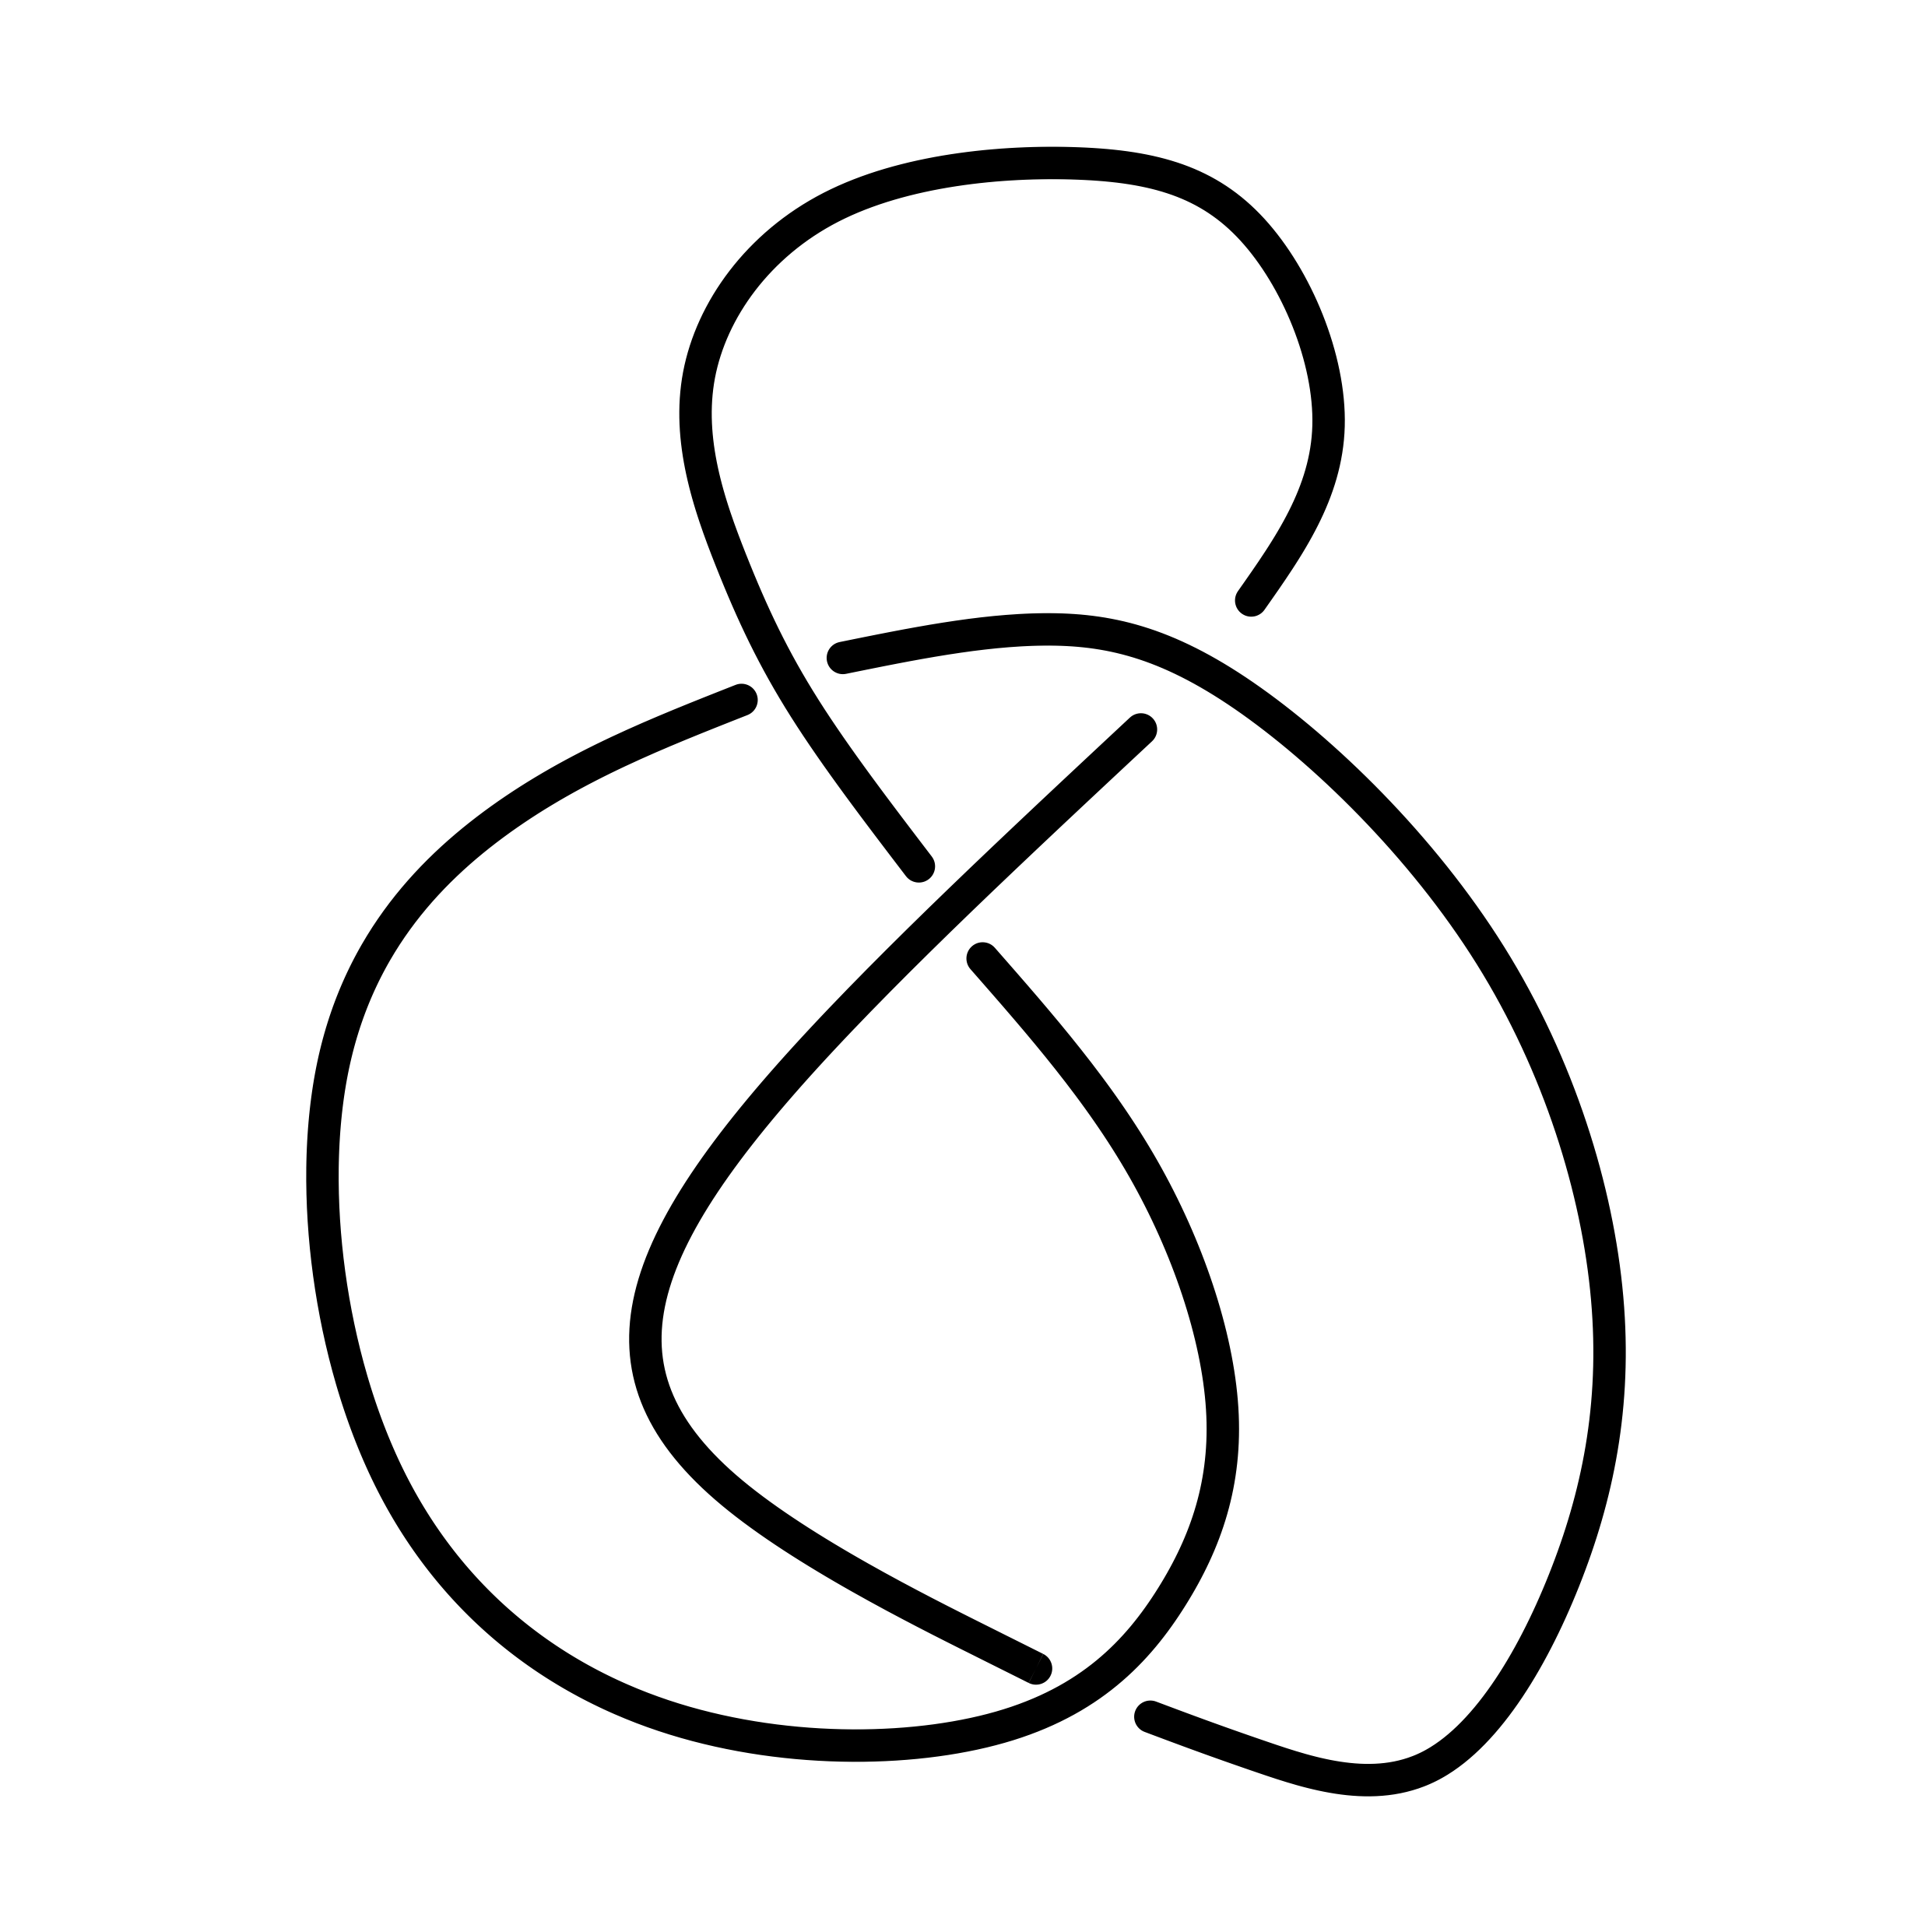
\includegraphics[width=0.4\linewidth]{picture/knotpict/knot-0}
		\caption{Figure-Eight Knot}
		\label{fig:mainmodel}
	\end{figure}
\newline
Then we define knot invariants,
\begin{defn} Knot Invariants:
	\begin{enumerate}
		\item function $f$ assigning to any knot diagram a number (a tuple of numbers, a polynomial, a rational function etc.
		\item for any two diagrams of the same knot f assigns the same number.
		\item Color the diagram into 3 colors. The coloring is correct if at each crossing,
		the three meeting arcs are either all of the same color, or all of the different
		colors.
		\item Coloring invariant $col_3$(D) is the number of correct colorings.
	\end{enumerate}
\end{defn}
we want to find every combination of coloring or numbering that satisfies 3-colorings or 3 "trivial" colorings from figure \ref{fig:mainmodel}.\\
\newpage
\textbf{Answer}.\\
The combination of coloring figure \ref{fig:mainmodel} is as follows:
\begin{figure}[h!]
	\begin{subfigure}[b]{0.25\linewidth}
		\centering
		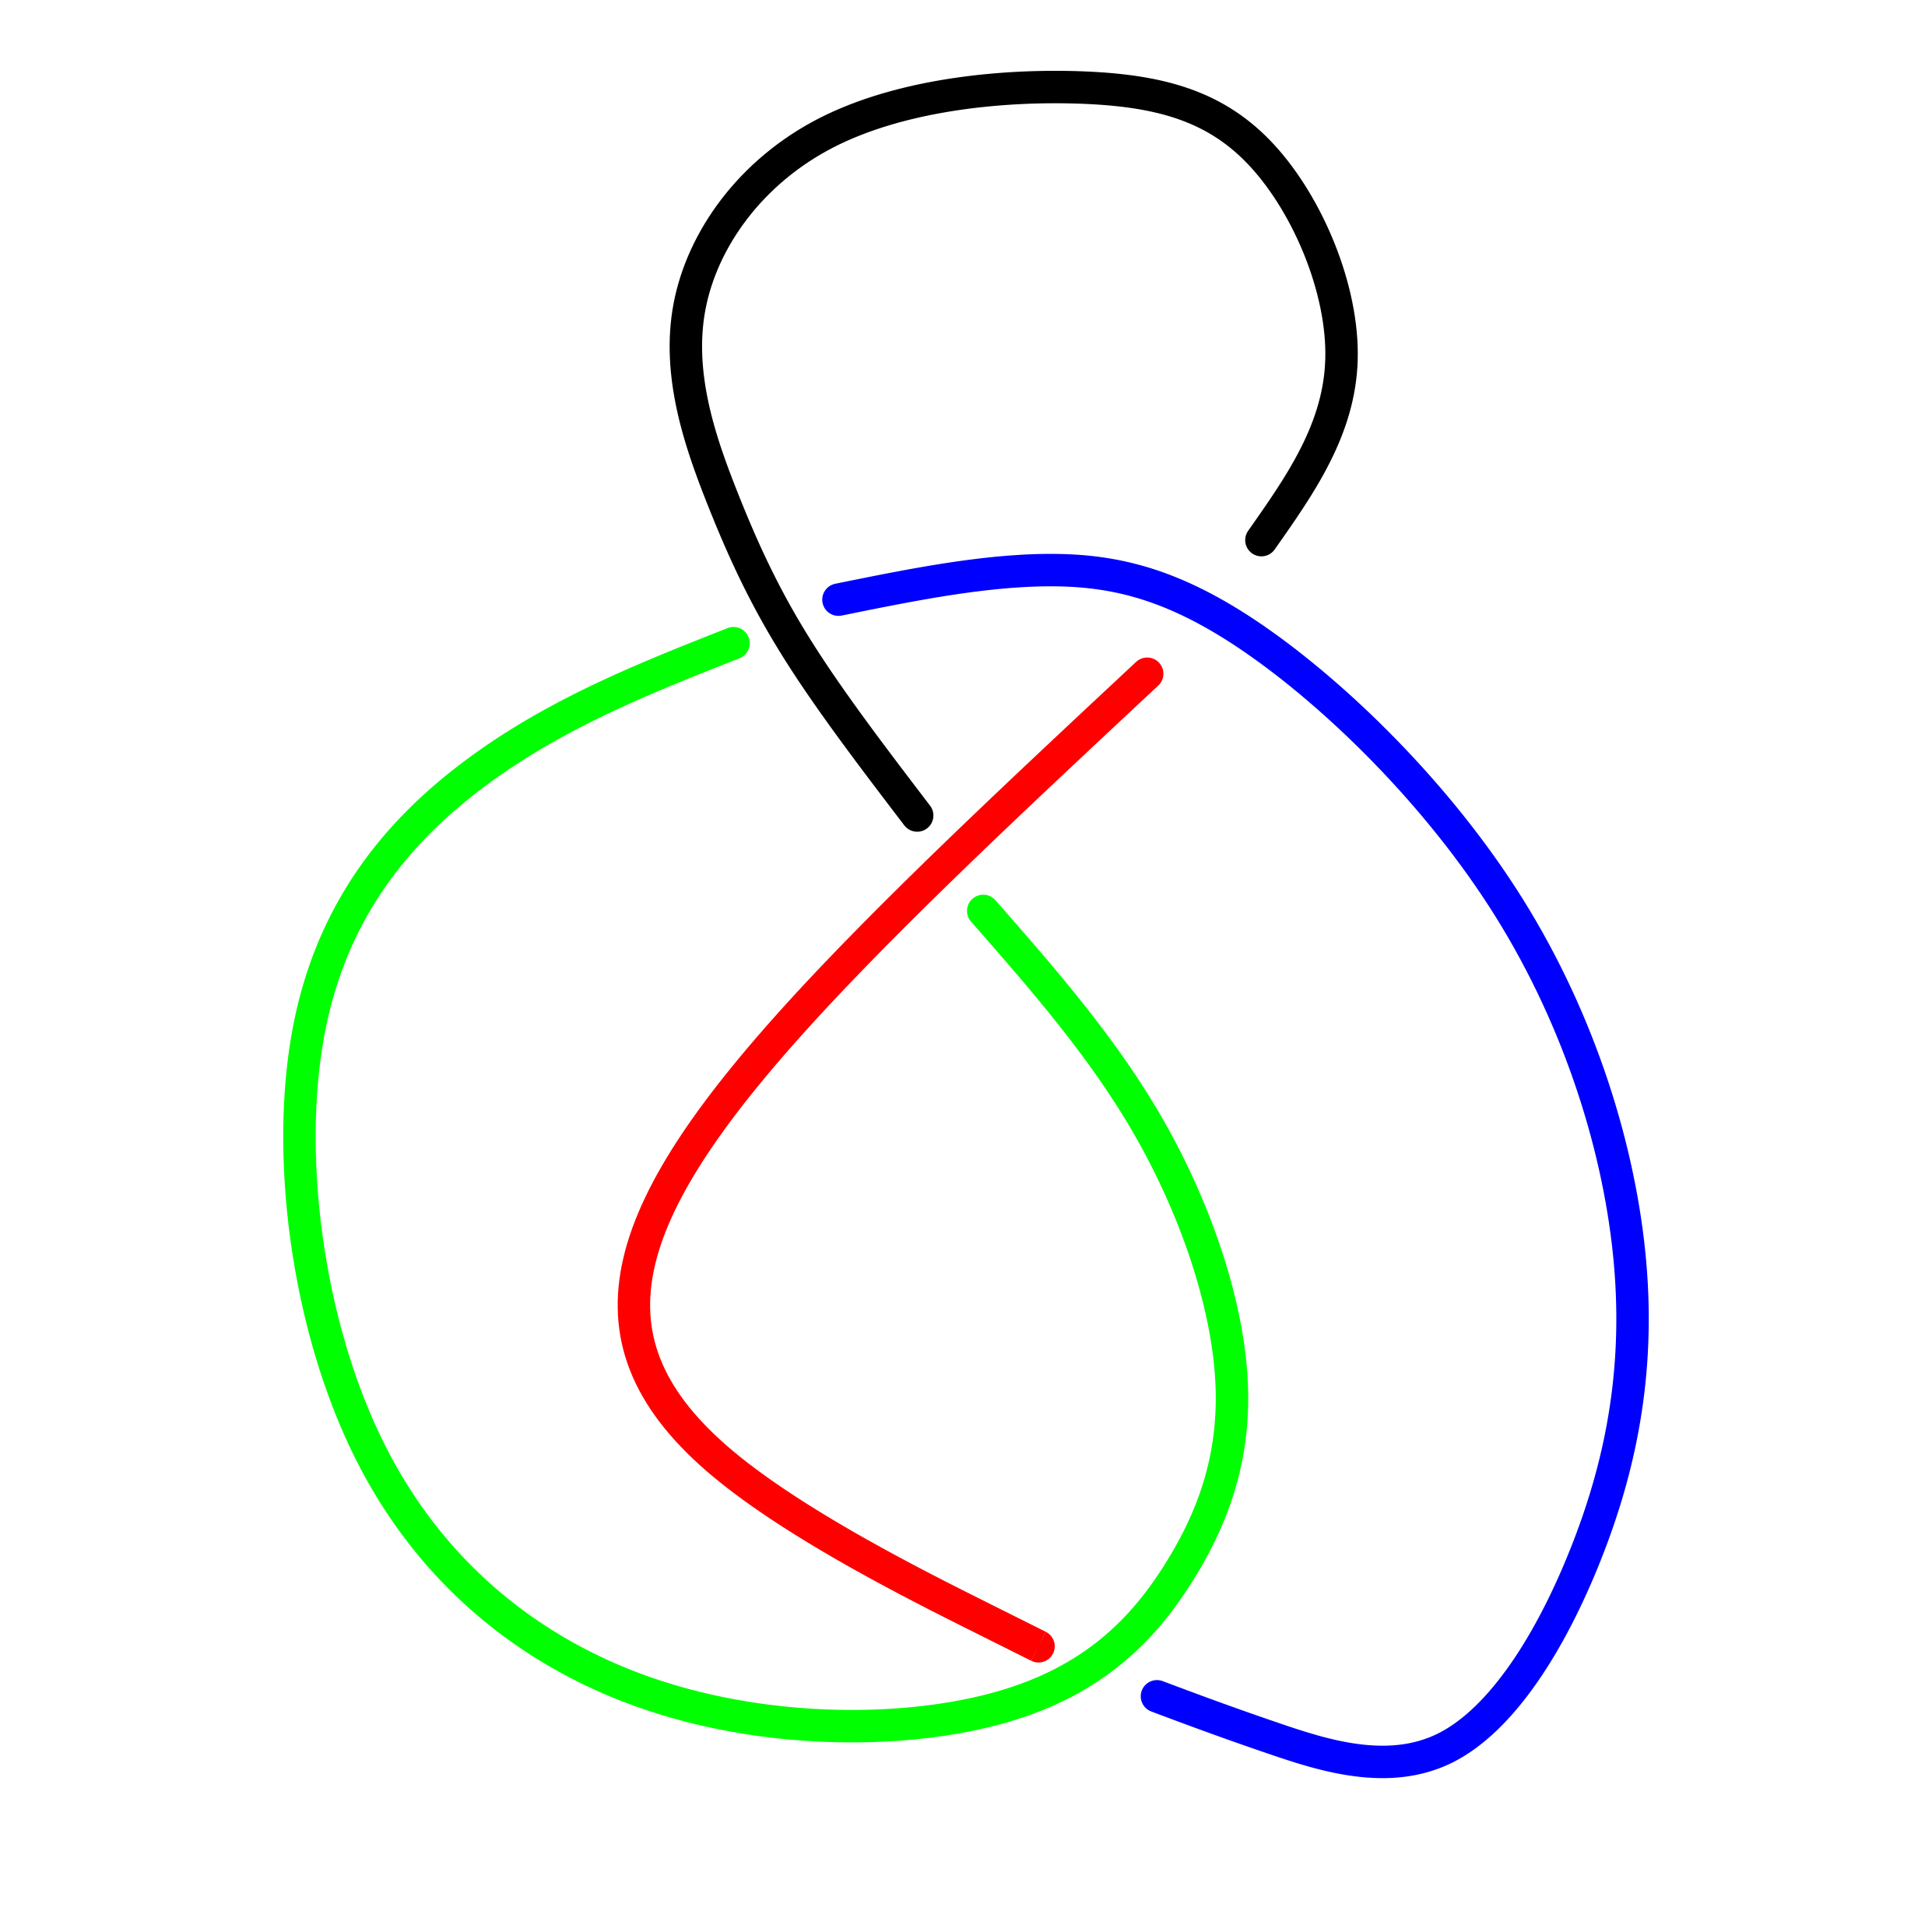
\includegraphics[width=0.5\linewidth]{picture/knotpict/knot-1}
		\caption{1st Combination}
	\end{subfigure}
	\qquad
	\begin{subfigure}[b]{0.25\linewidth}
		\centering
		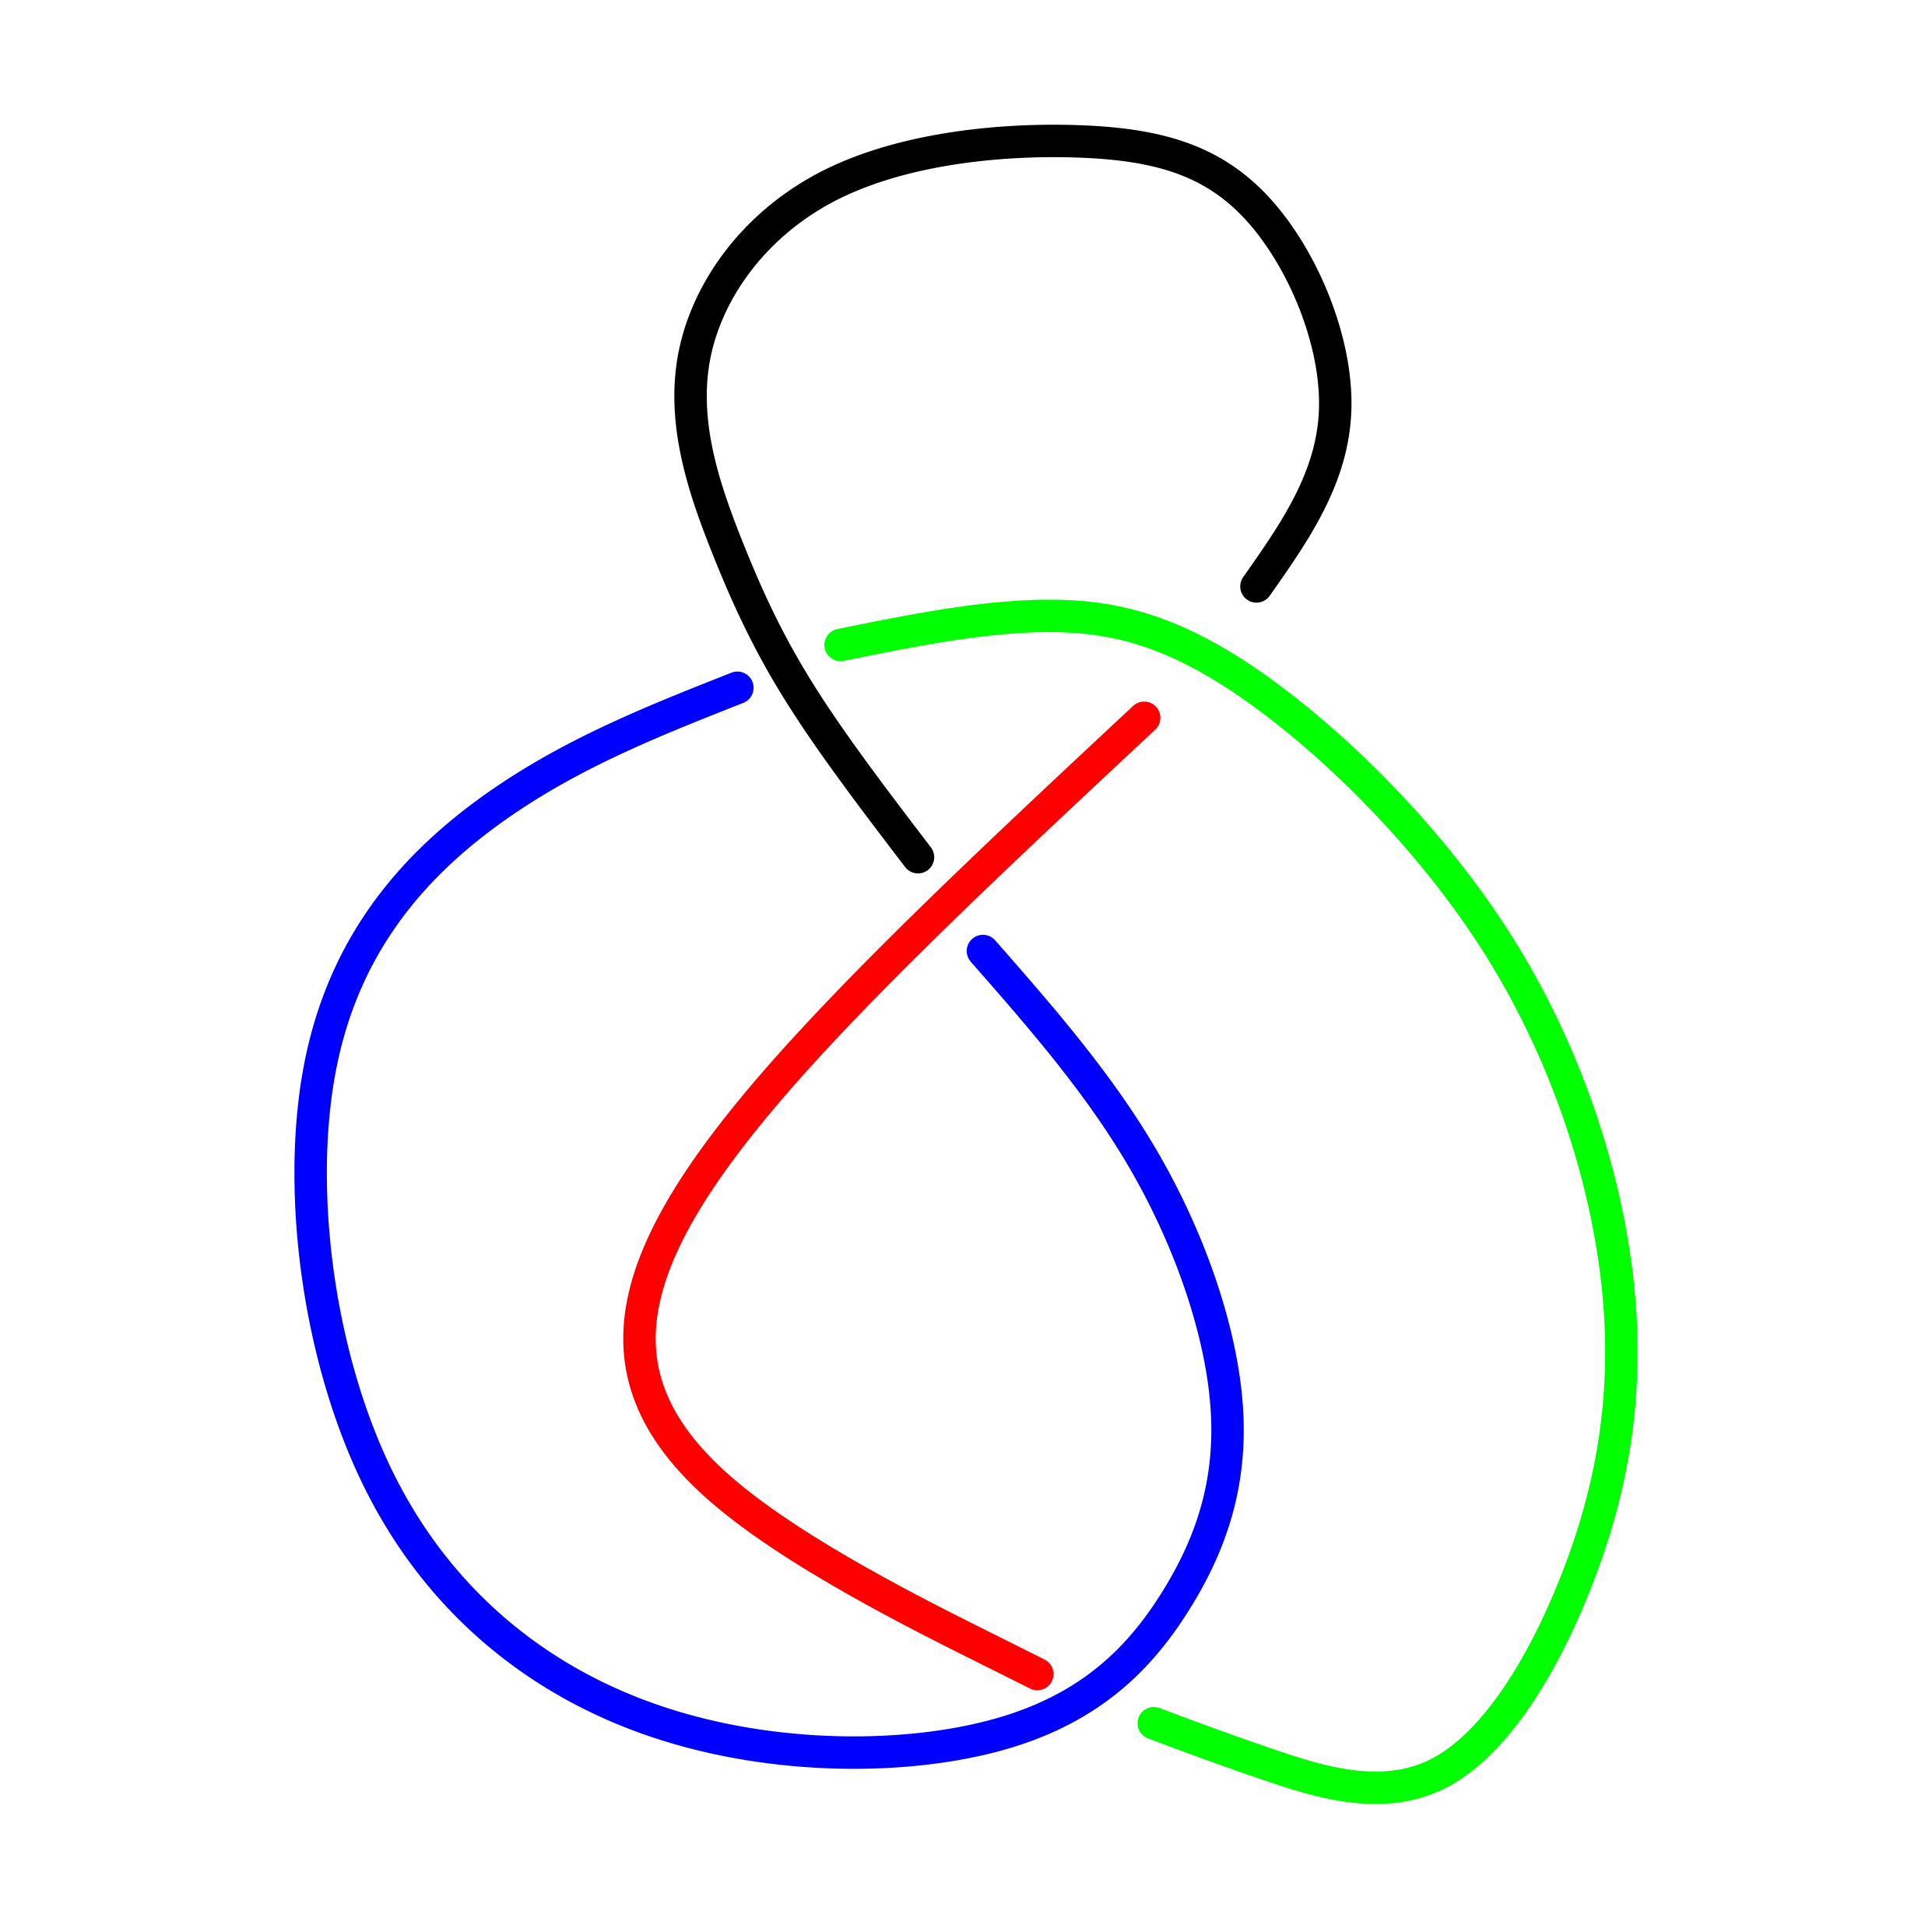
\includegraphics[width=0.5\linewidth]{picture/knotpict/knot-2}
		\caption{2nd Combination}
	\end{subfigure}
	\qquad
	\begin{subfigure}[b]{0.25\linewidth}
		\centering
		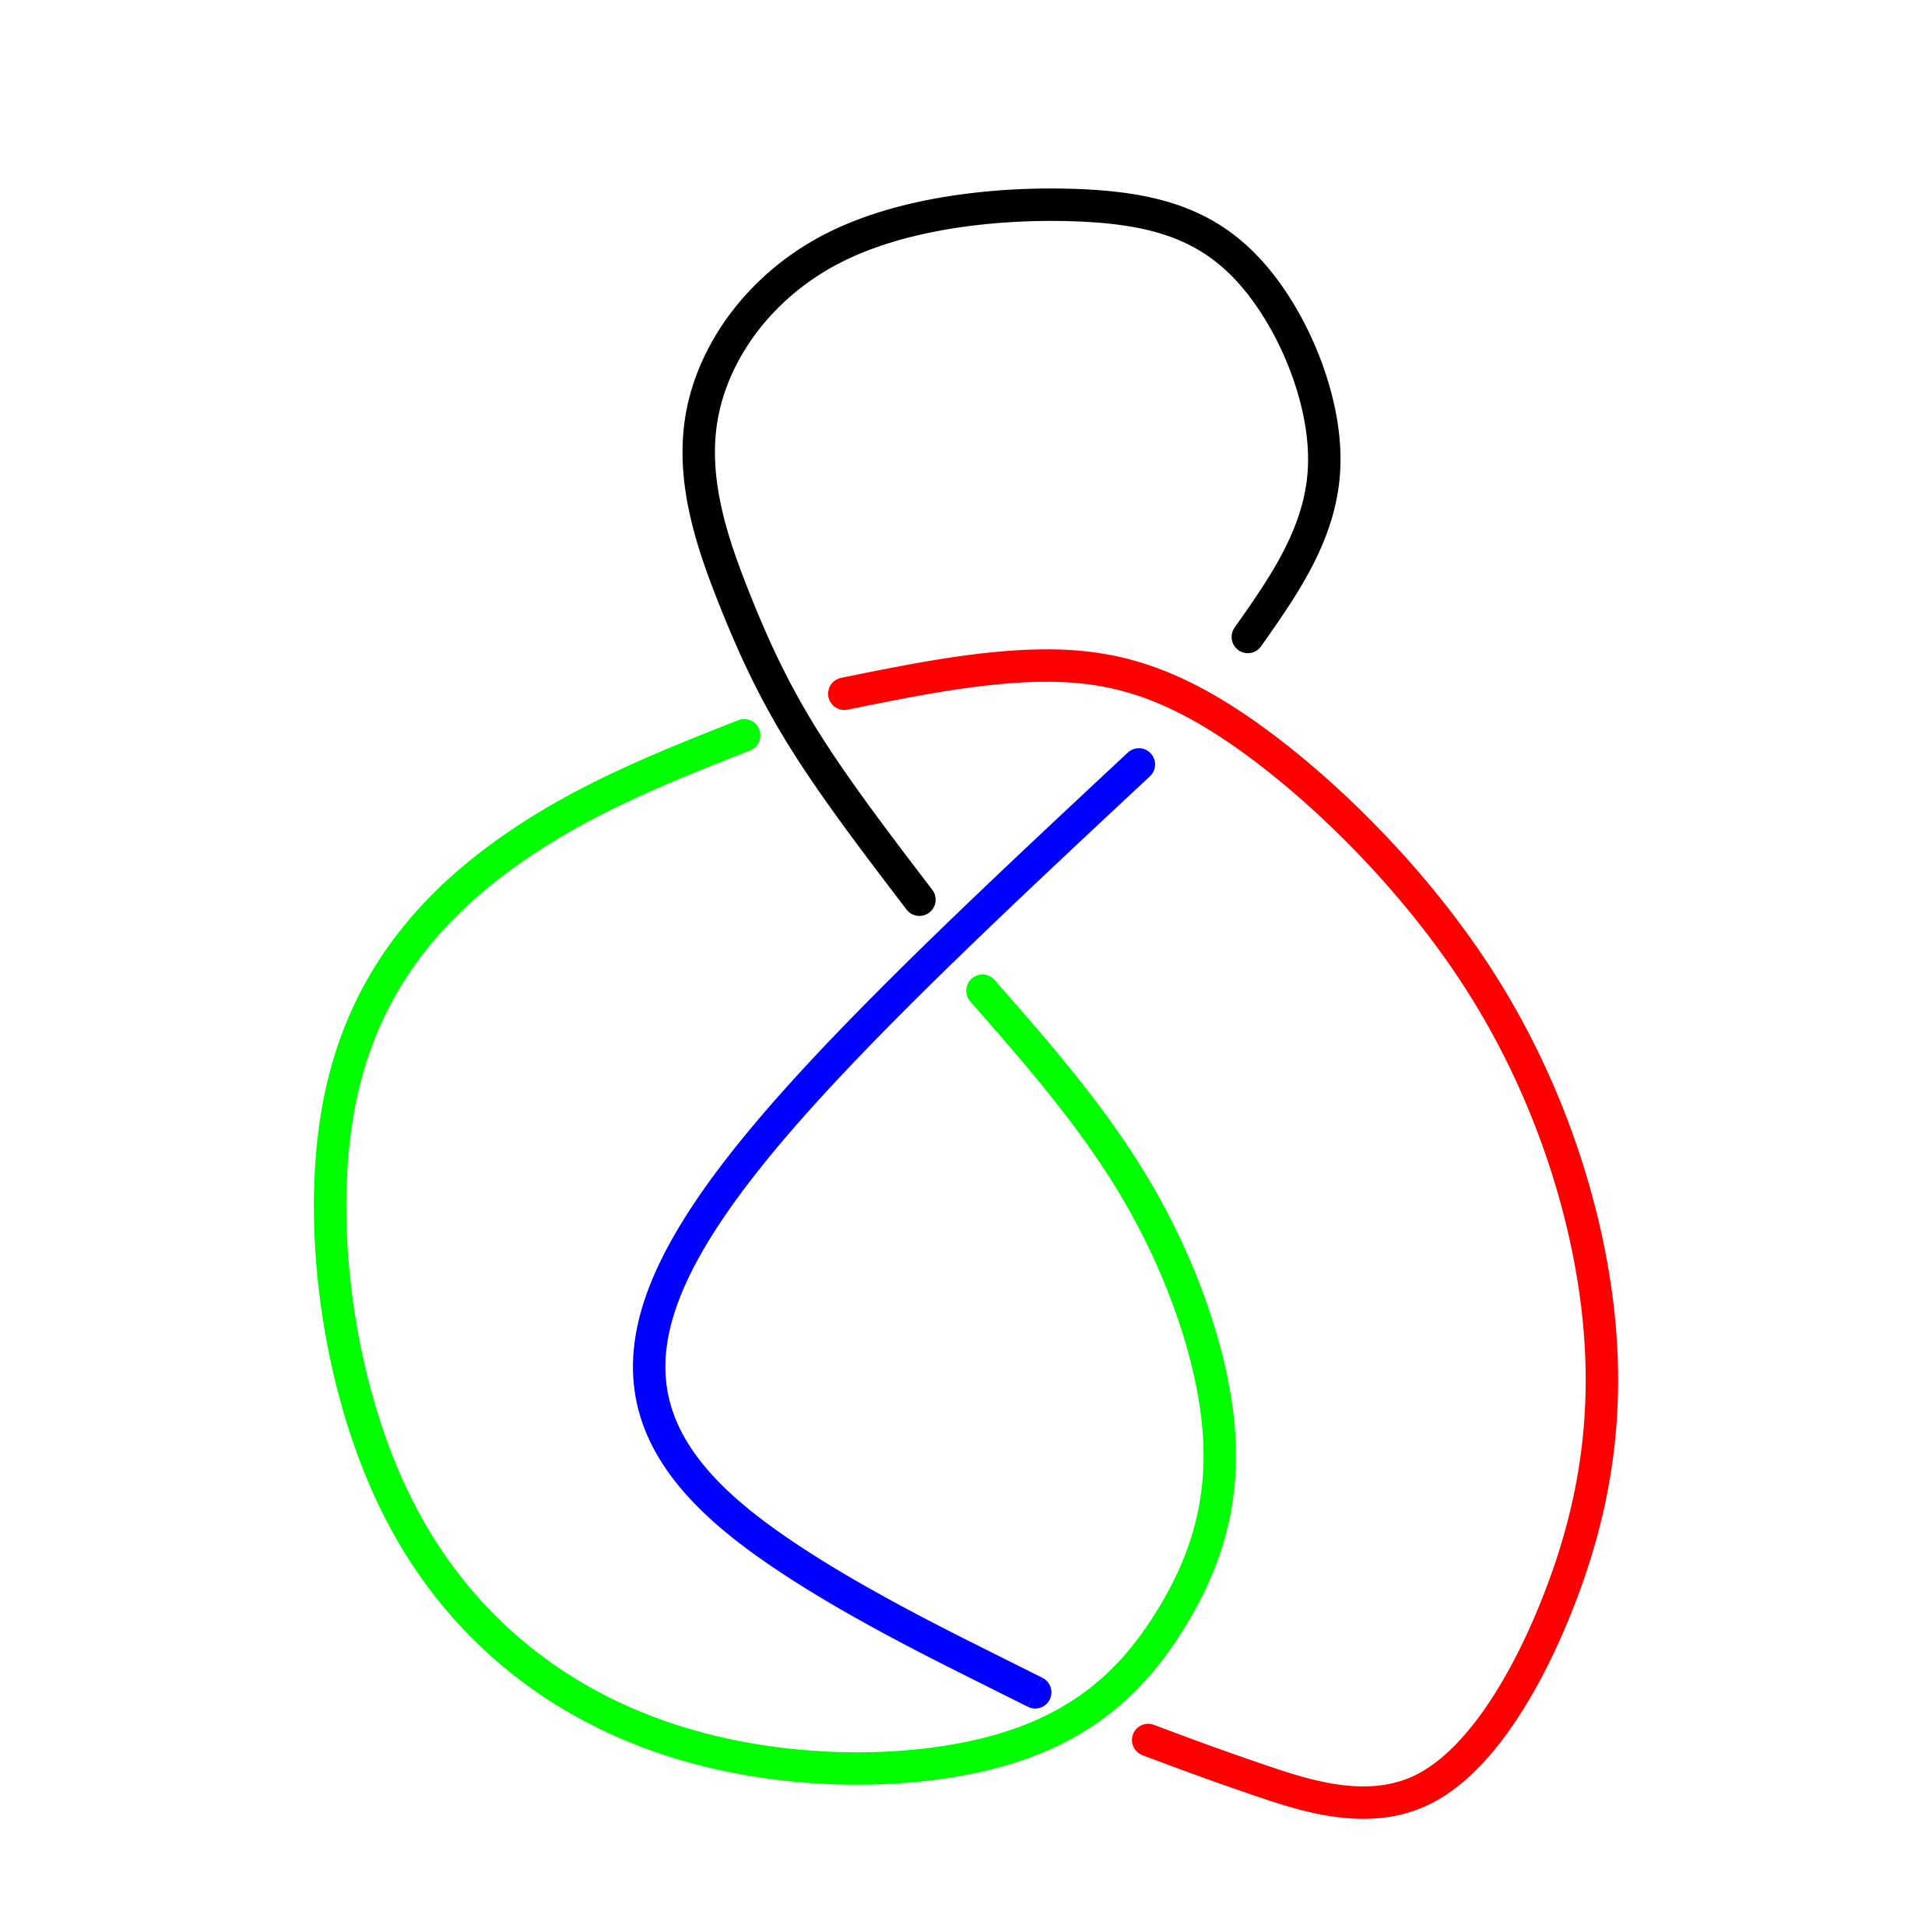
\includegraphics[width=0.5\linewidth]{picture/knotpict/knot-3}
		\caption{3rd Combination}
	\end{subfigure}
	\qquad
	\begin{subfigure}[b]{0.25\linewidth}
		\centering
		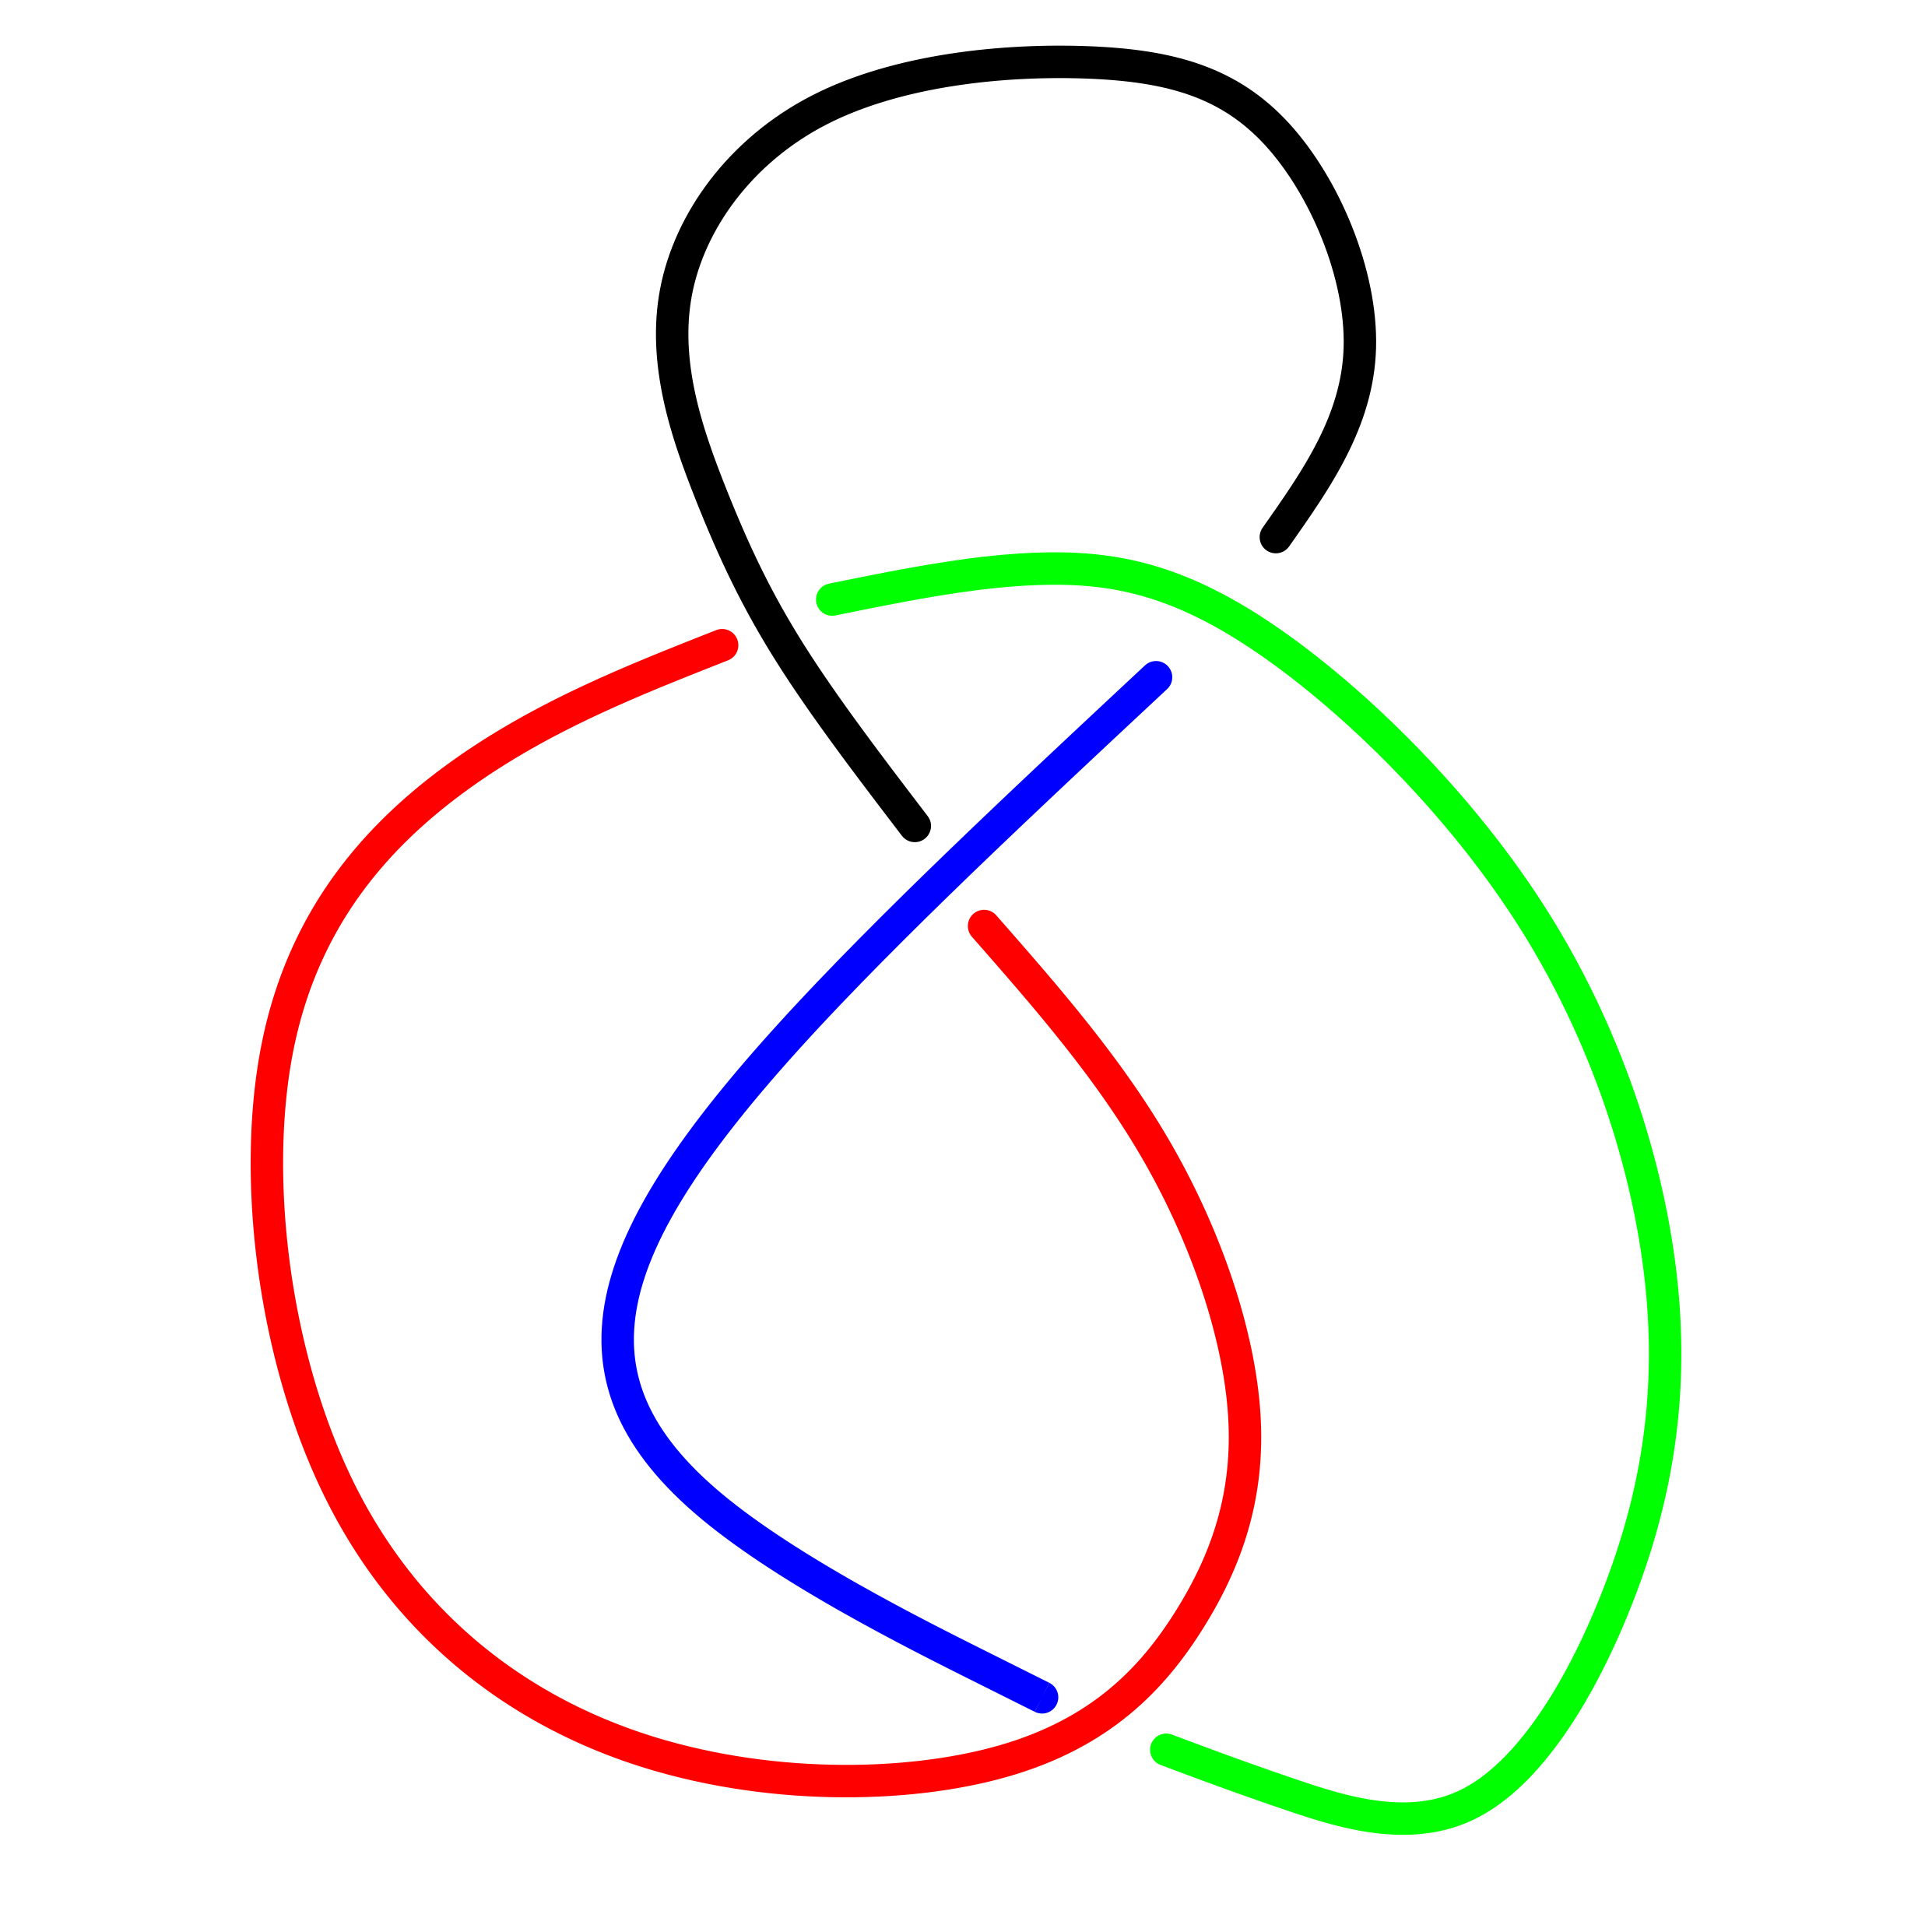
\includegraphics[width=0.5\linewidth]{picture/knotpict/knot-4}
		\caption{4th Combination}
	\end{subfigure}
\qquad
\begin{subfigure}[b]{0.25\linewidth}
	\centering
	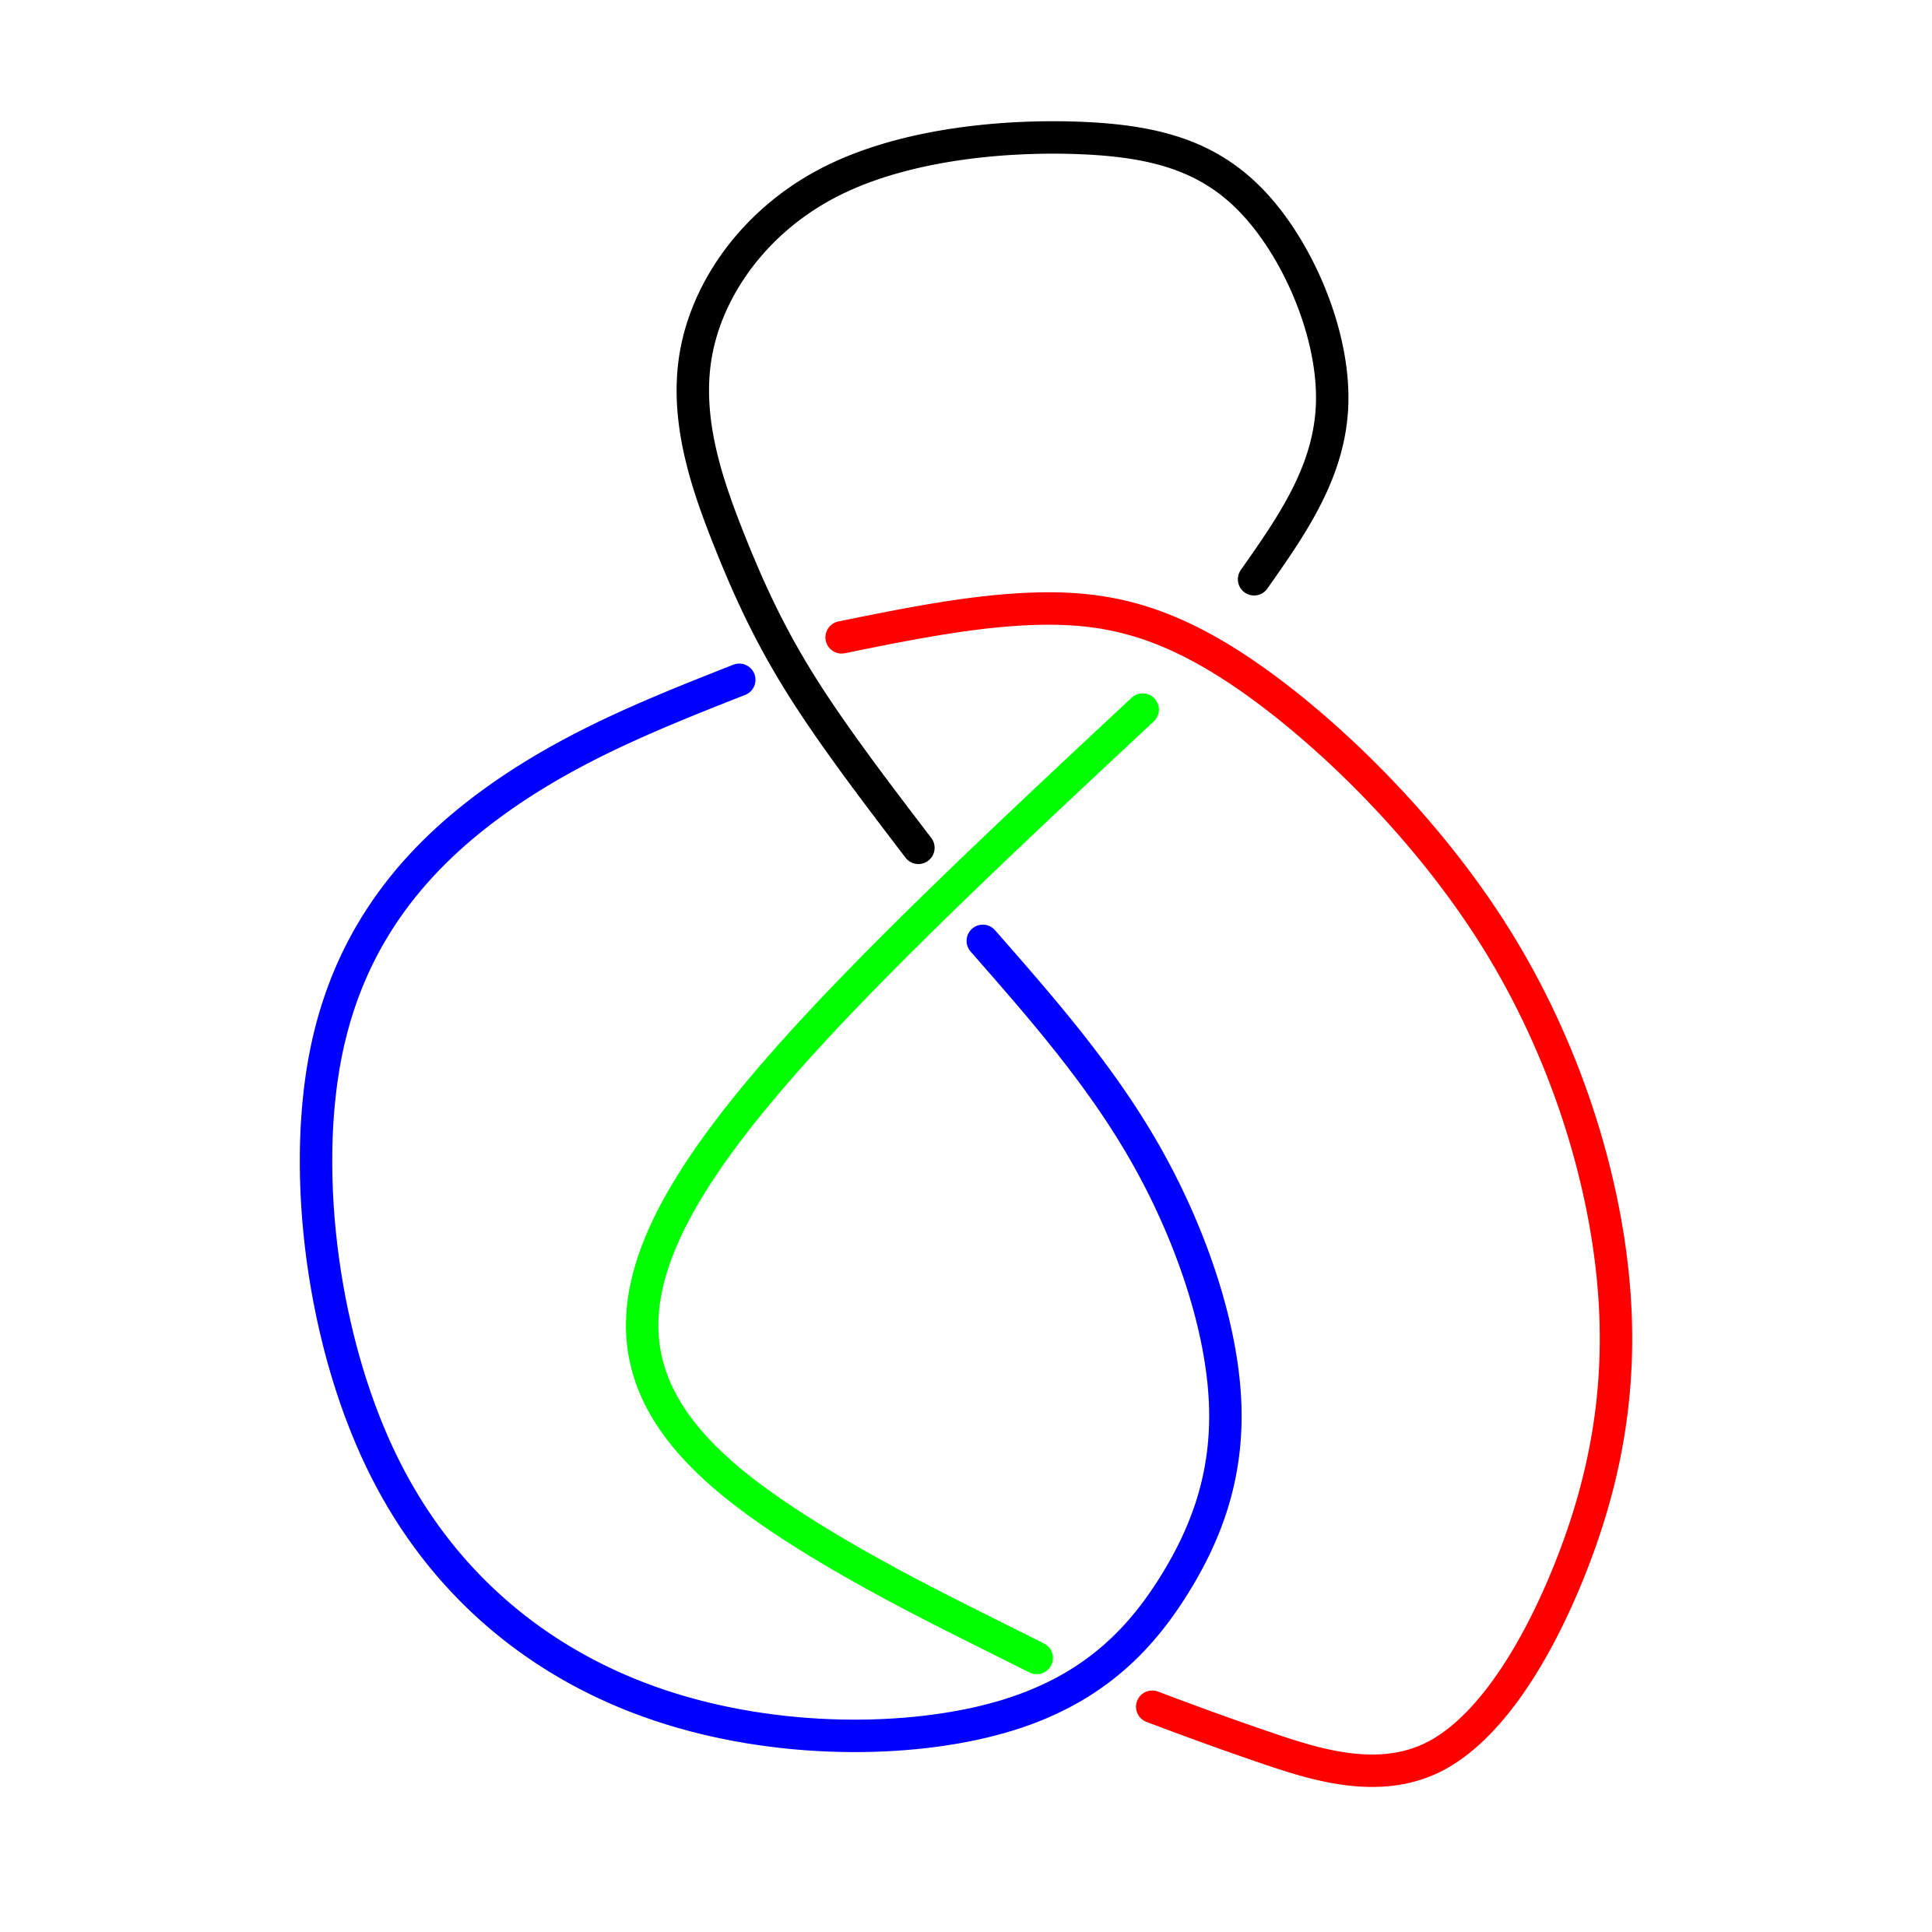
\includegraphics[width=0.5\linewidth]{picture/knotpict/knot-5}
	\caption{5th Combination}
\end{subfigure}
\qquad
\begin{subfigure}[b]{0.25\linewidth}
	\centering
	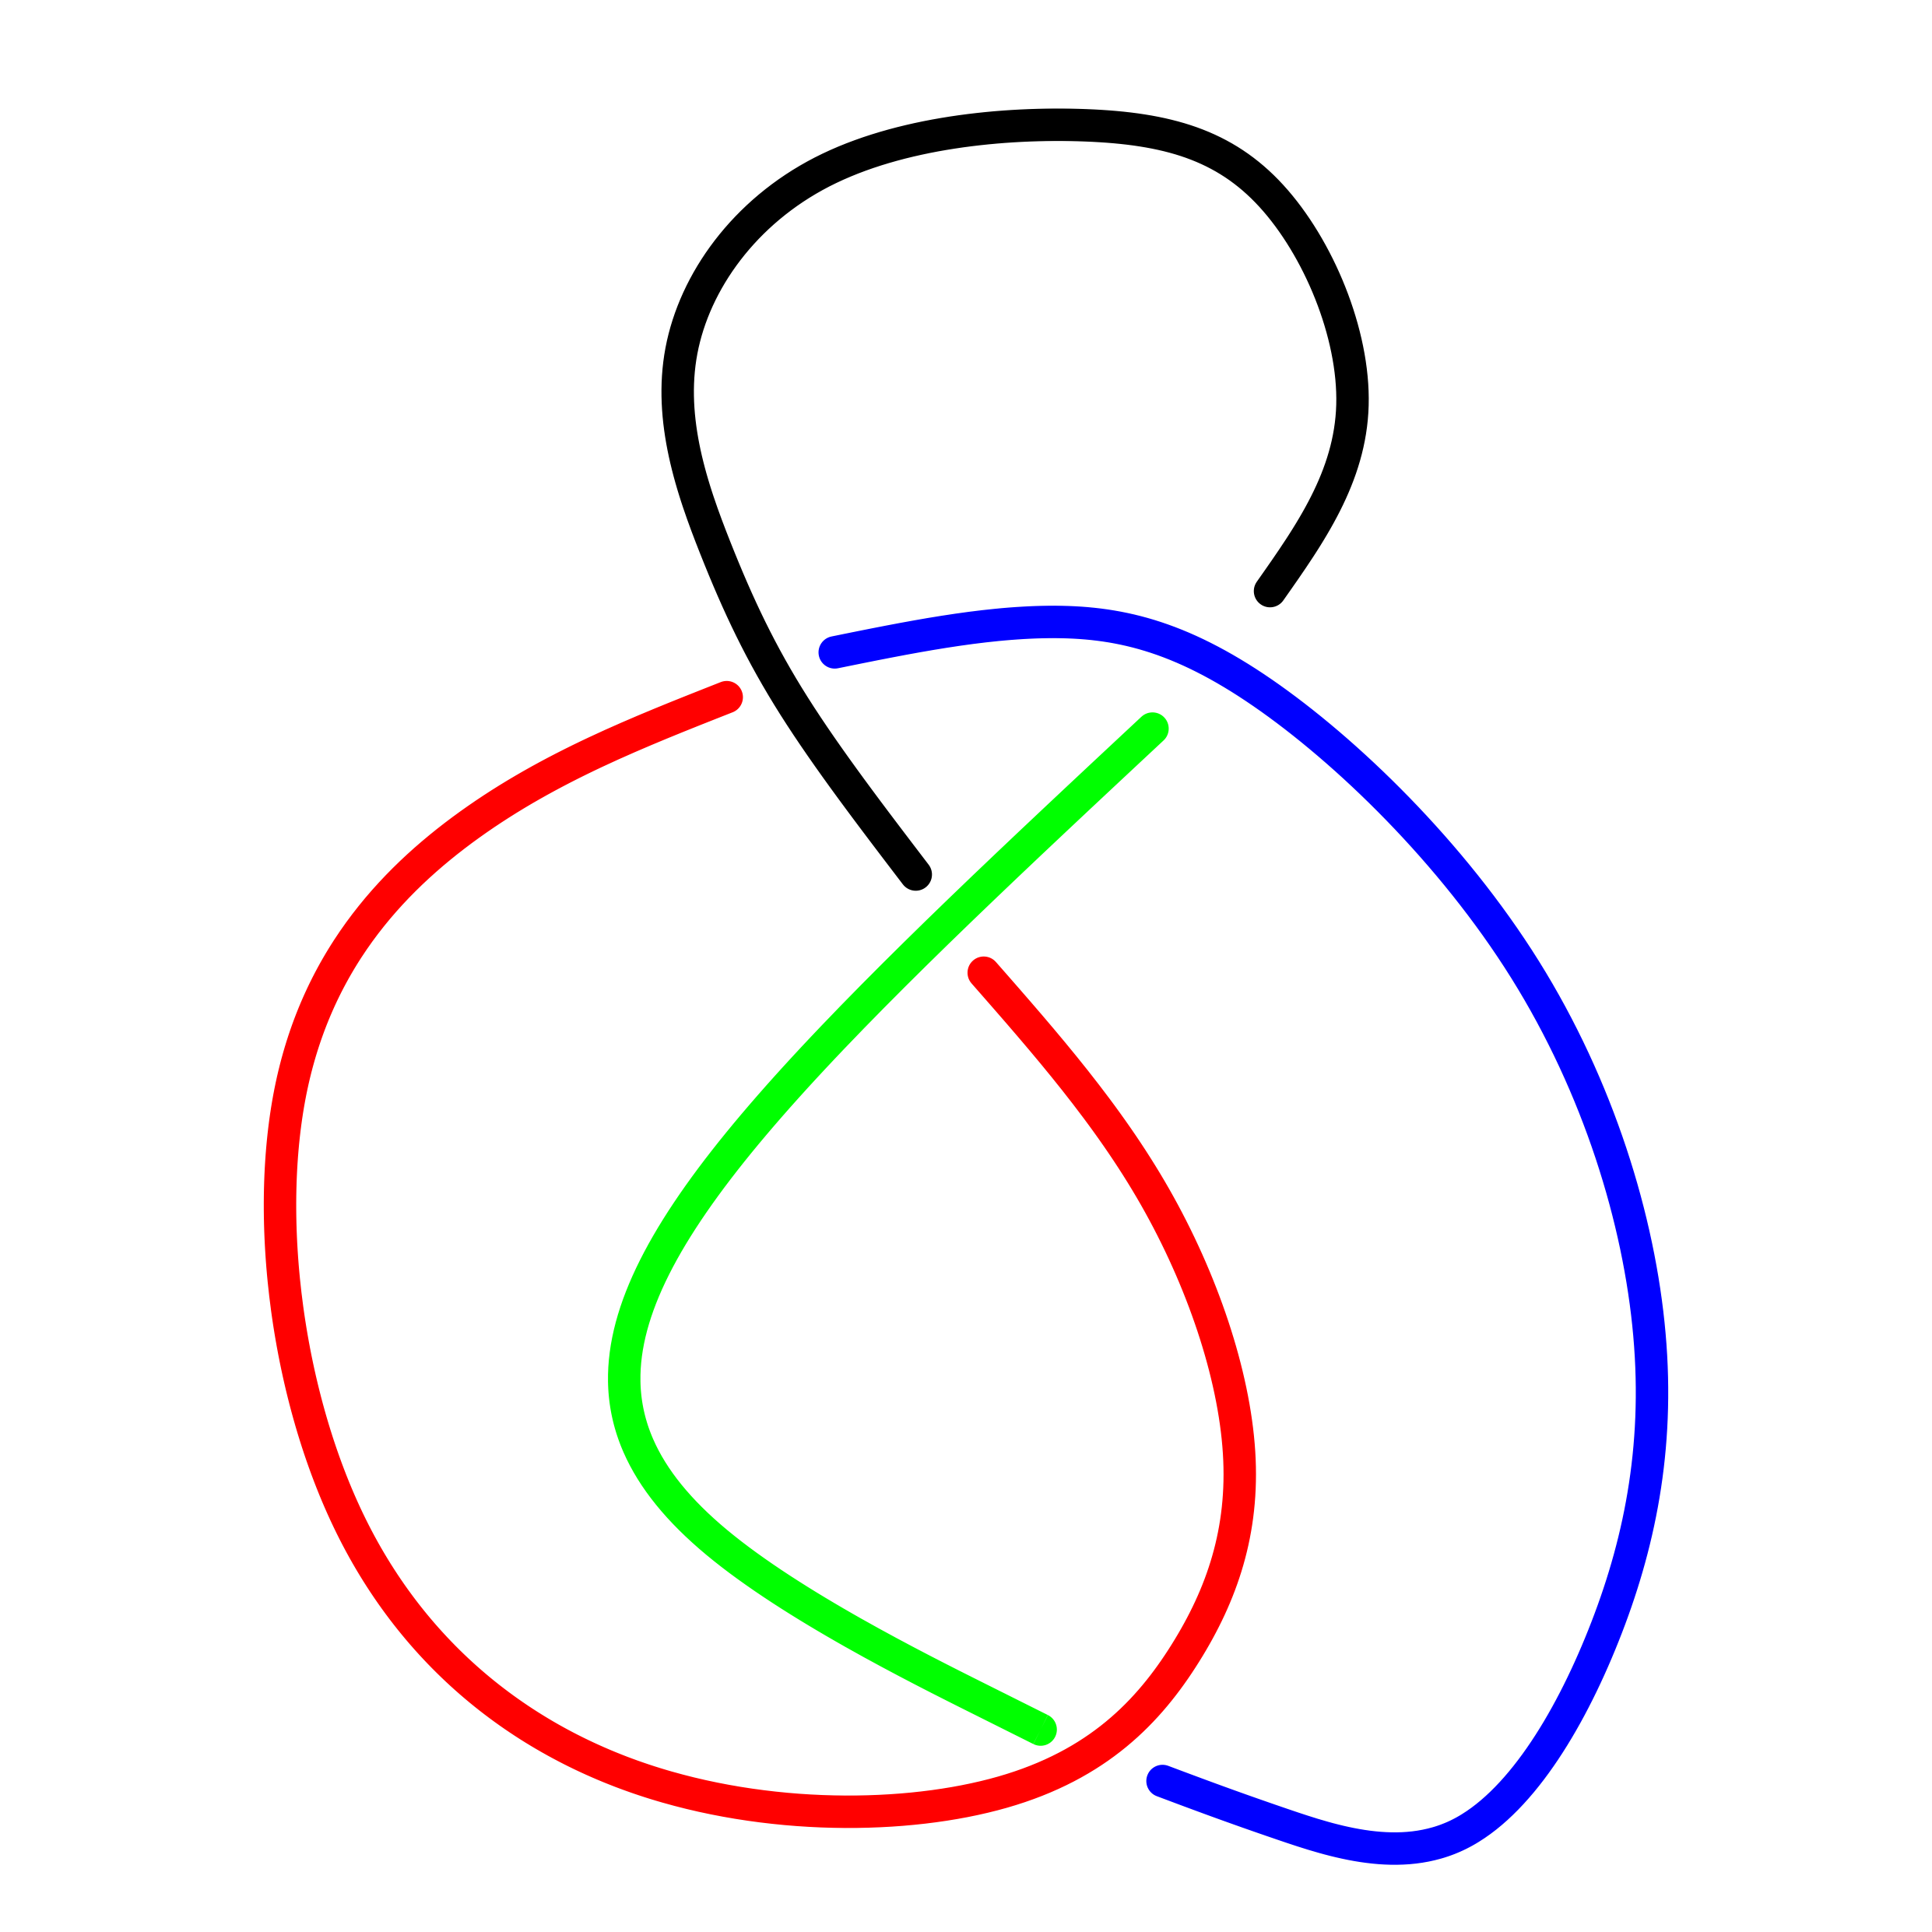
\includegraphics[width=0.5\linewidth]{picture/knotpict/knot-6}
	\caption{6th Combination}
\end{subfigure}
\qquad
\begin{subfigure}[b]{0.25\linewidth}
	\centering
	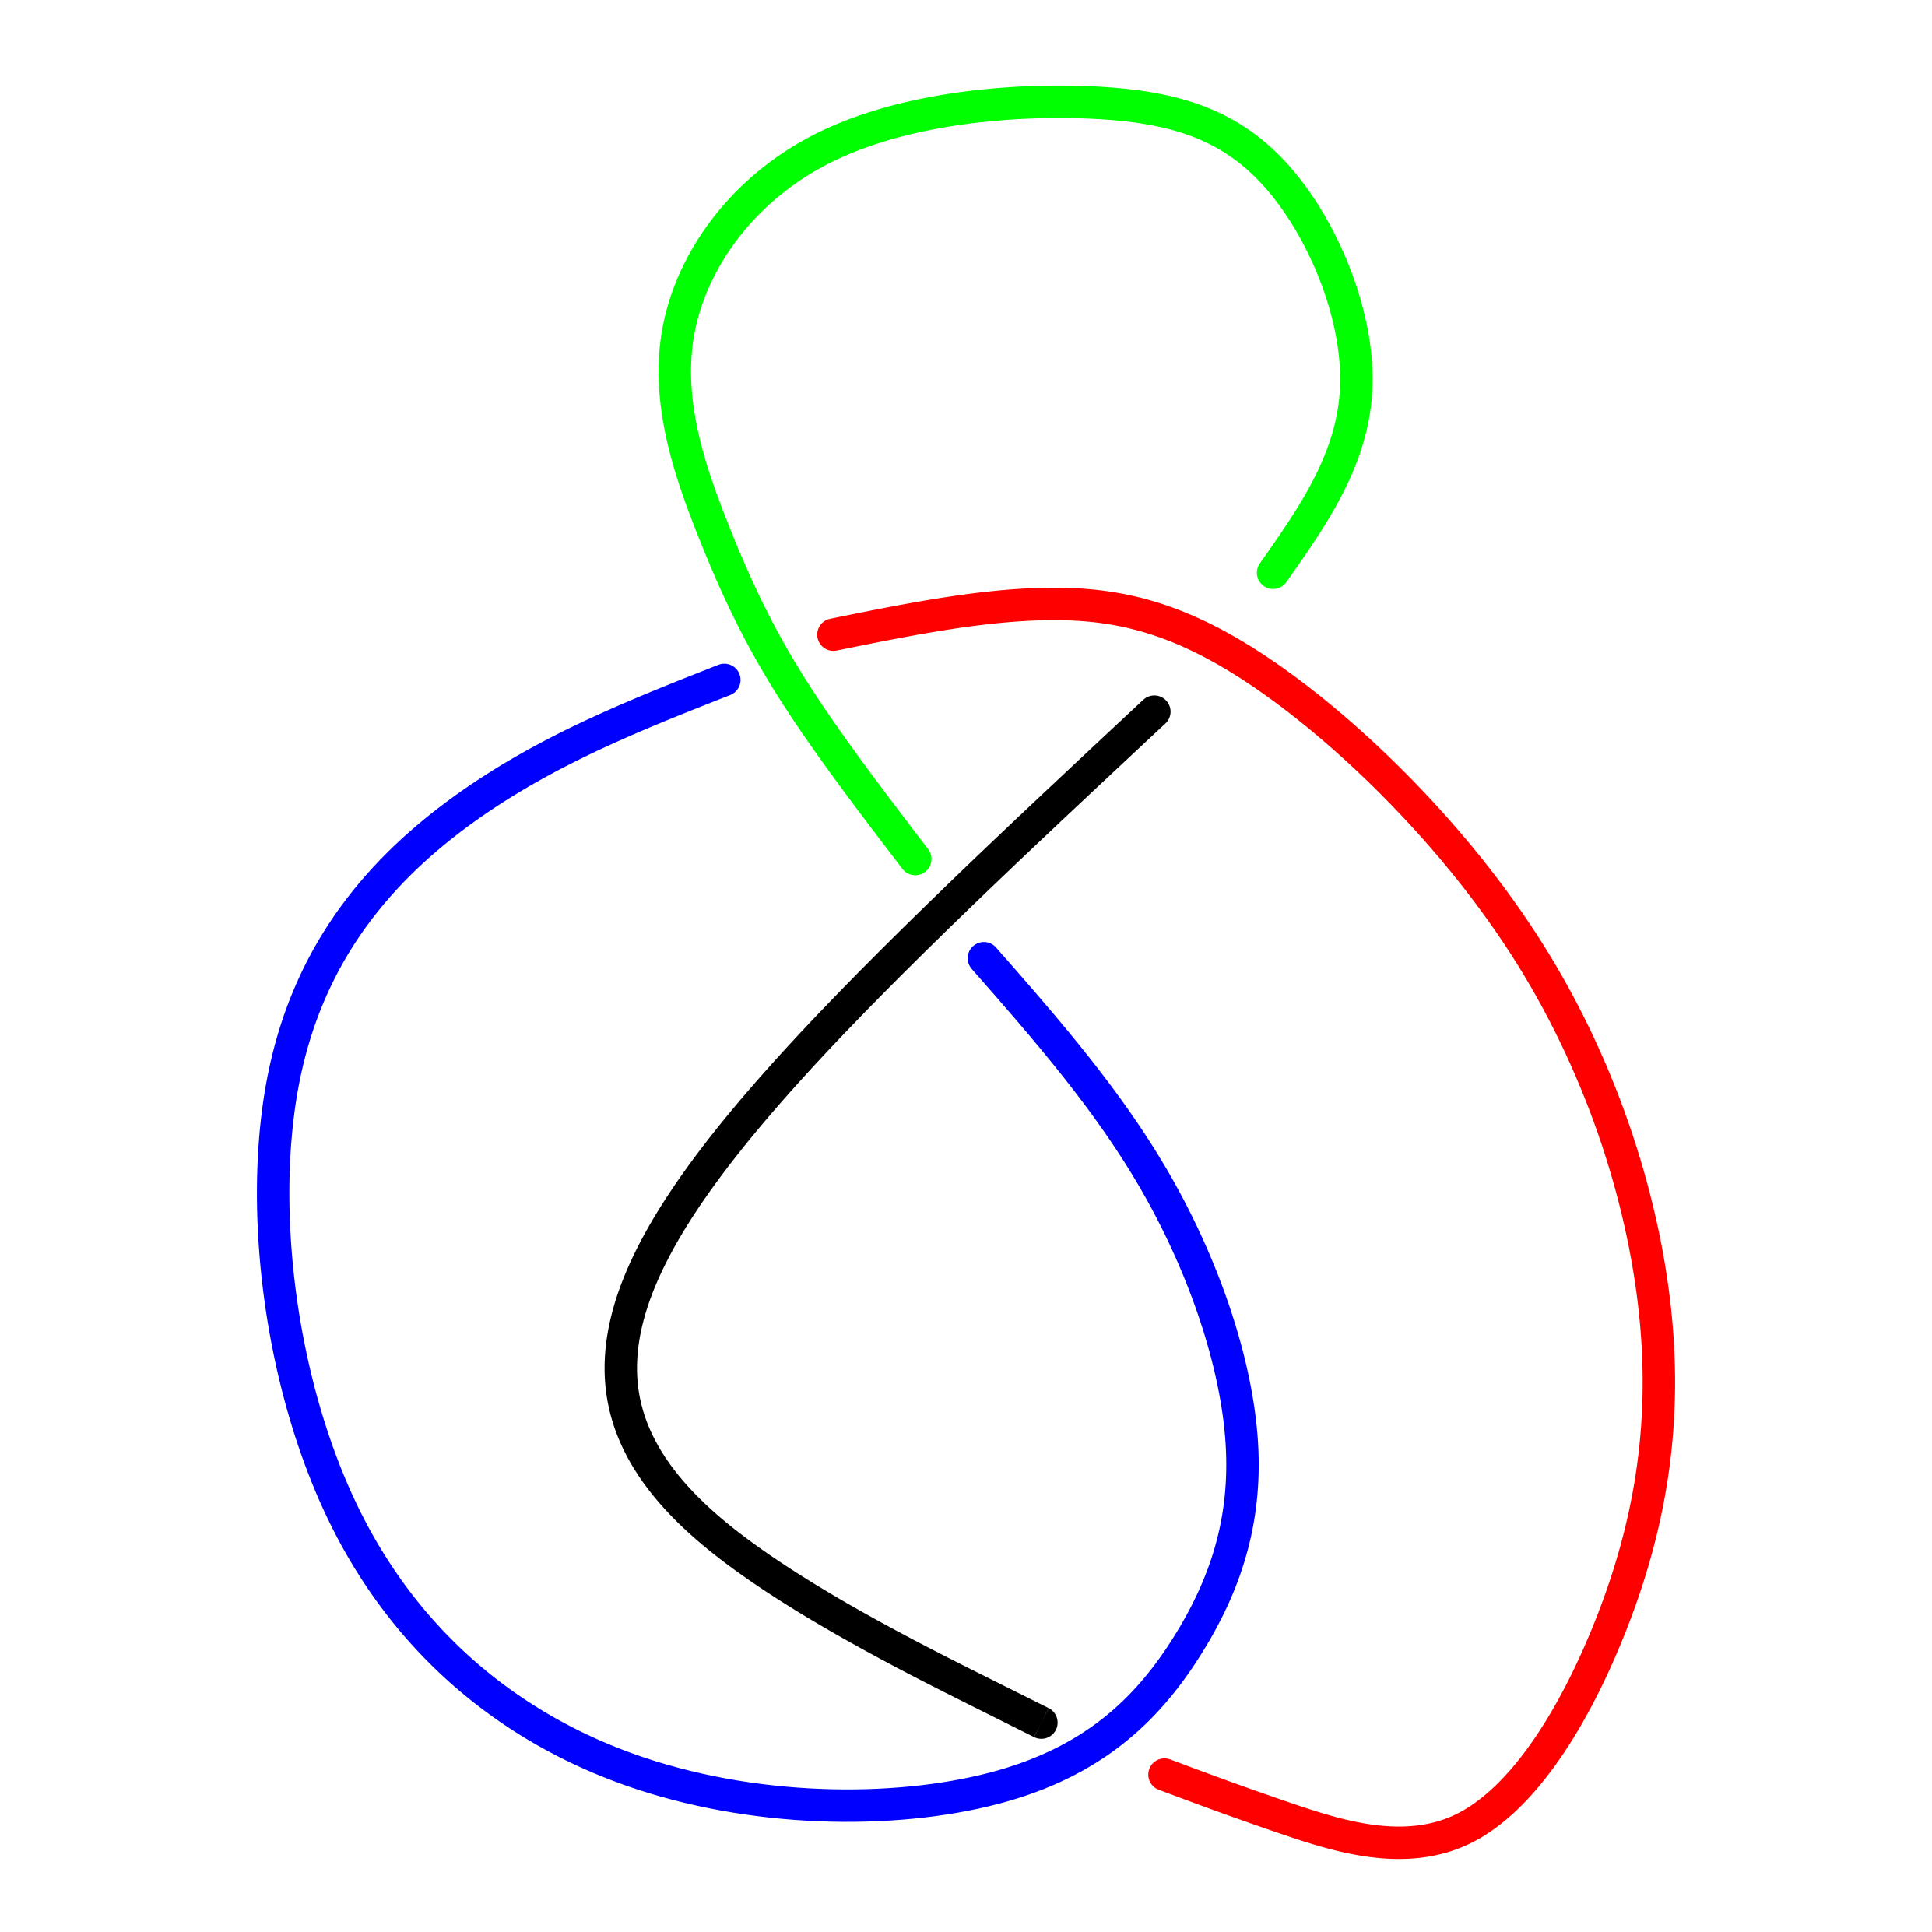
\includegraphics[width=0.5\linewidth]{picture/knotpict/knot-7}
	\caption{7th Combination}
\end{subfigure}
\qquad
\begin{subfigure}[b]{0.25\linewidth}
	\centering
	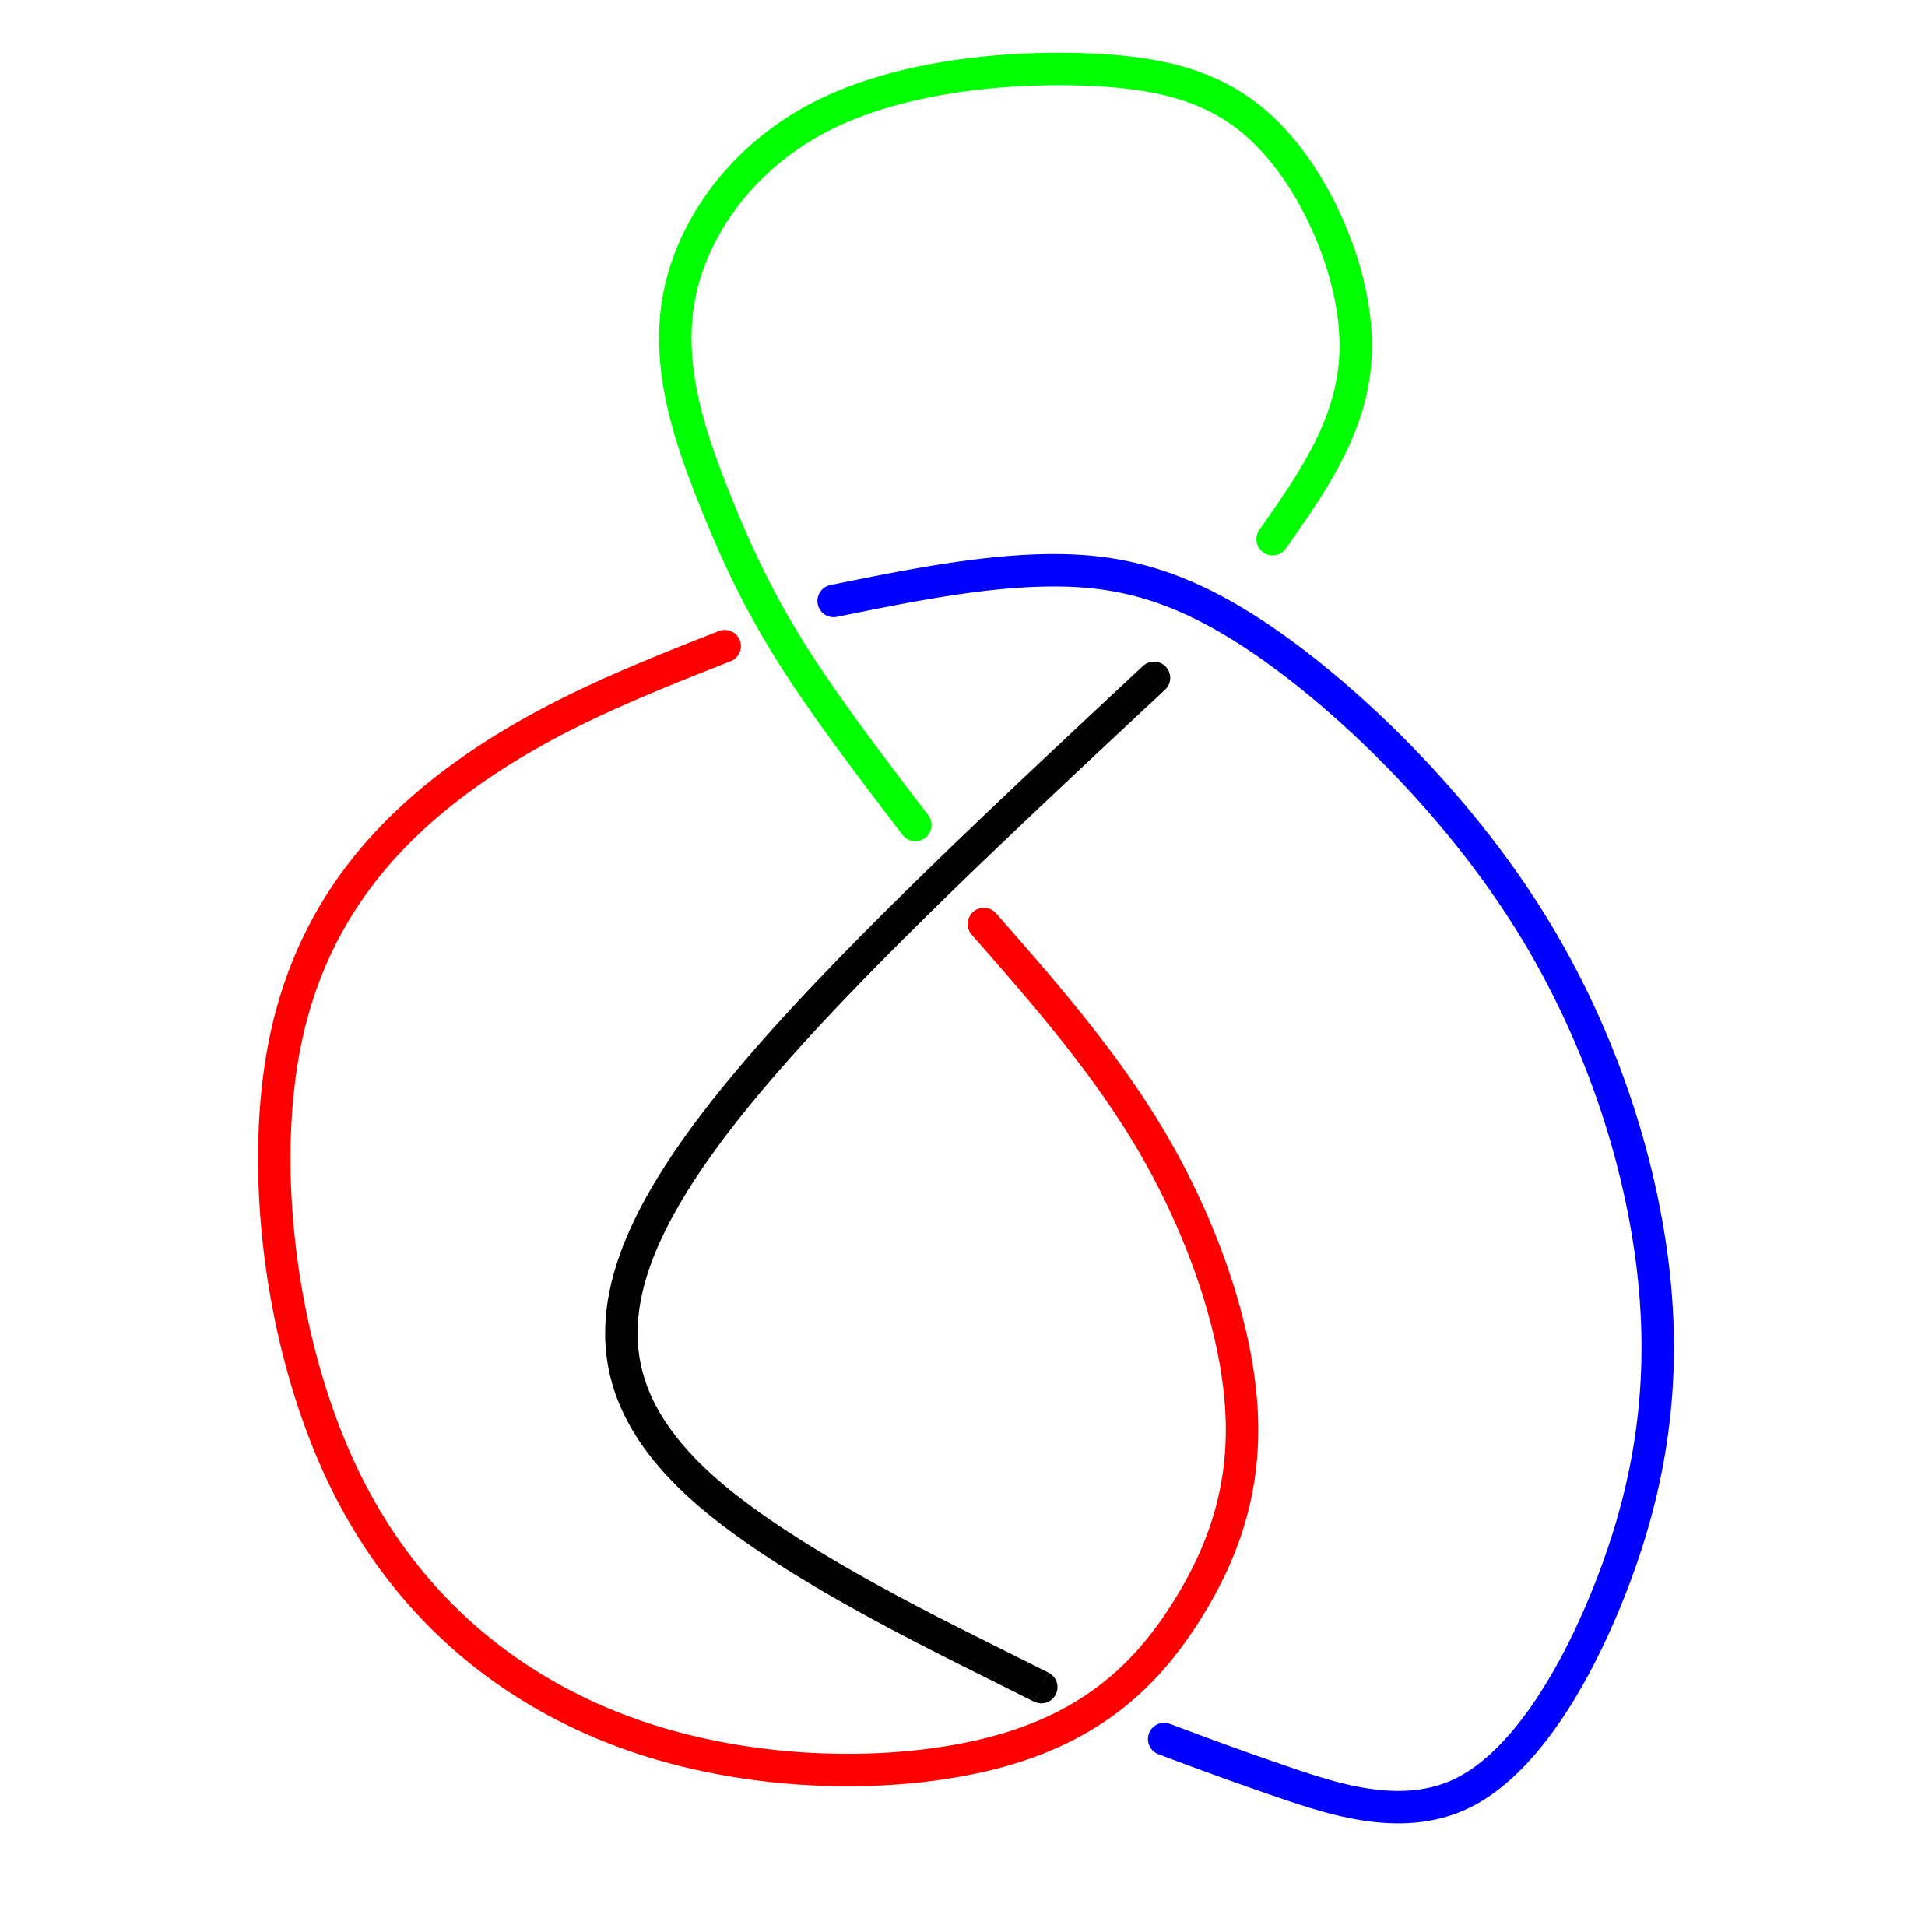
\includegraphics[width=0.5\linewidth]{picture/knotpict/knot-8}
	\caption{8th Combination}
\end{subfigure}
\qquad
\begin{subfigure}[b]{0.25\linewidth}
	\centering
	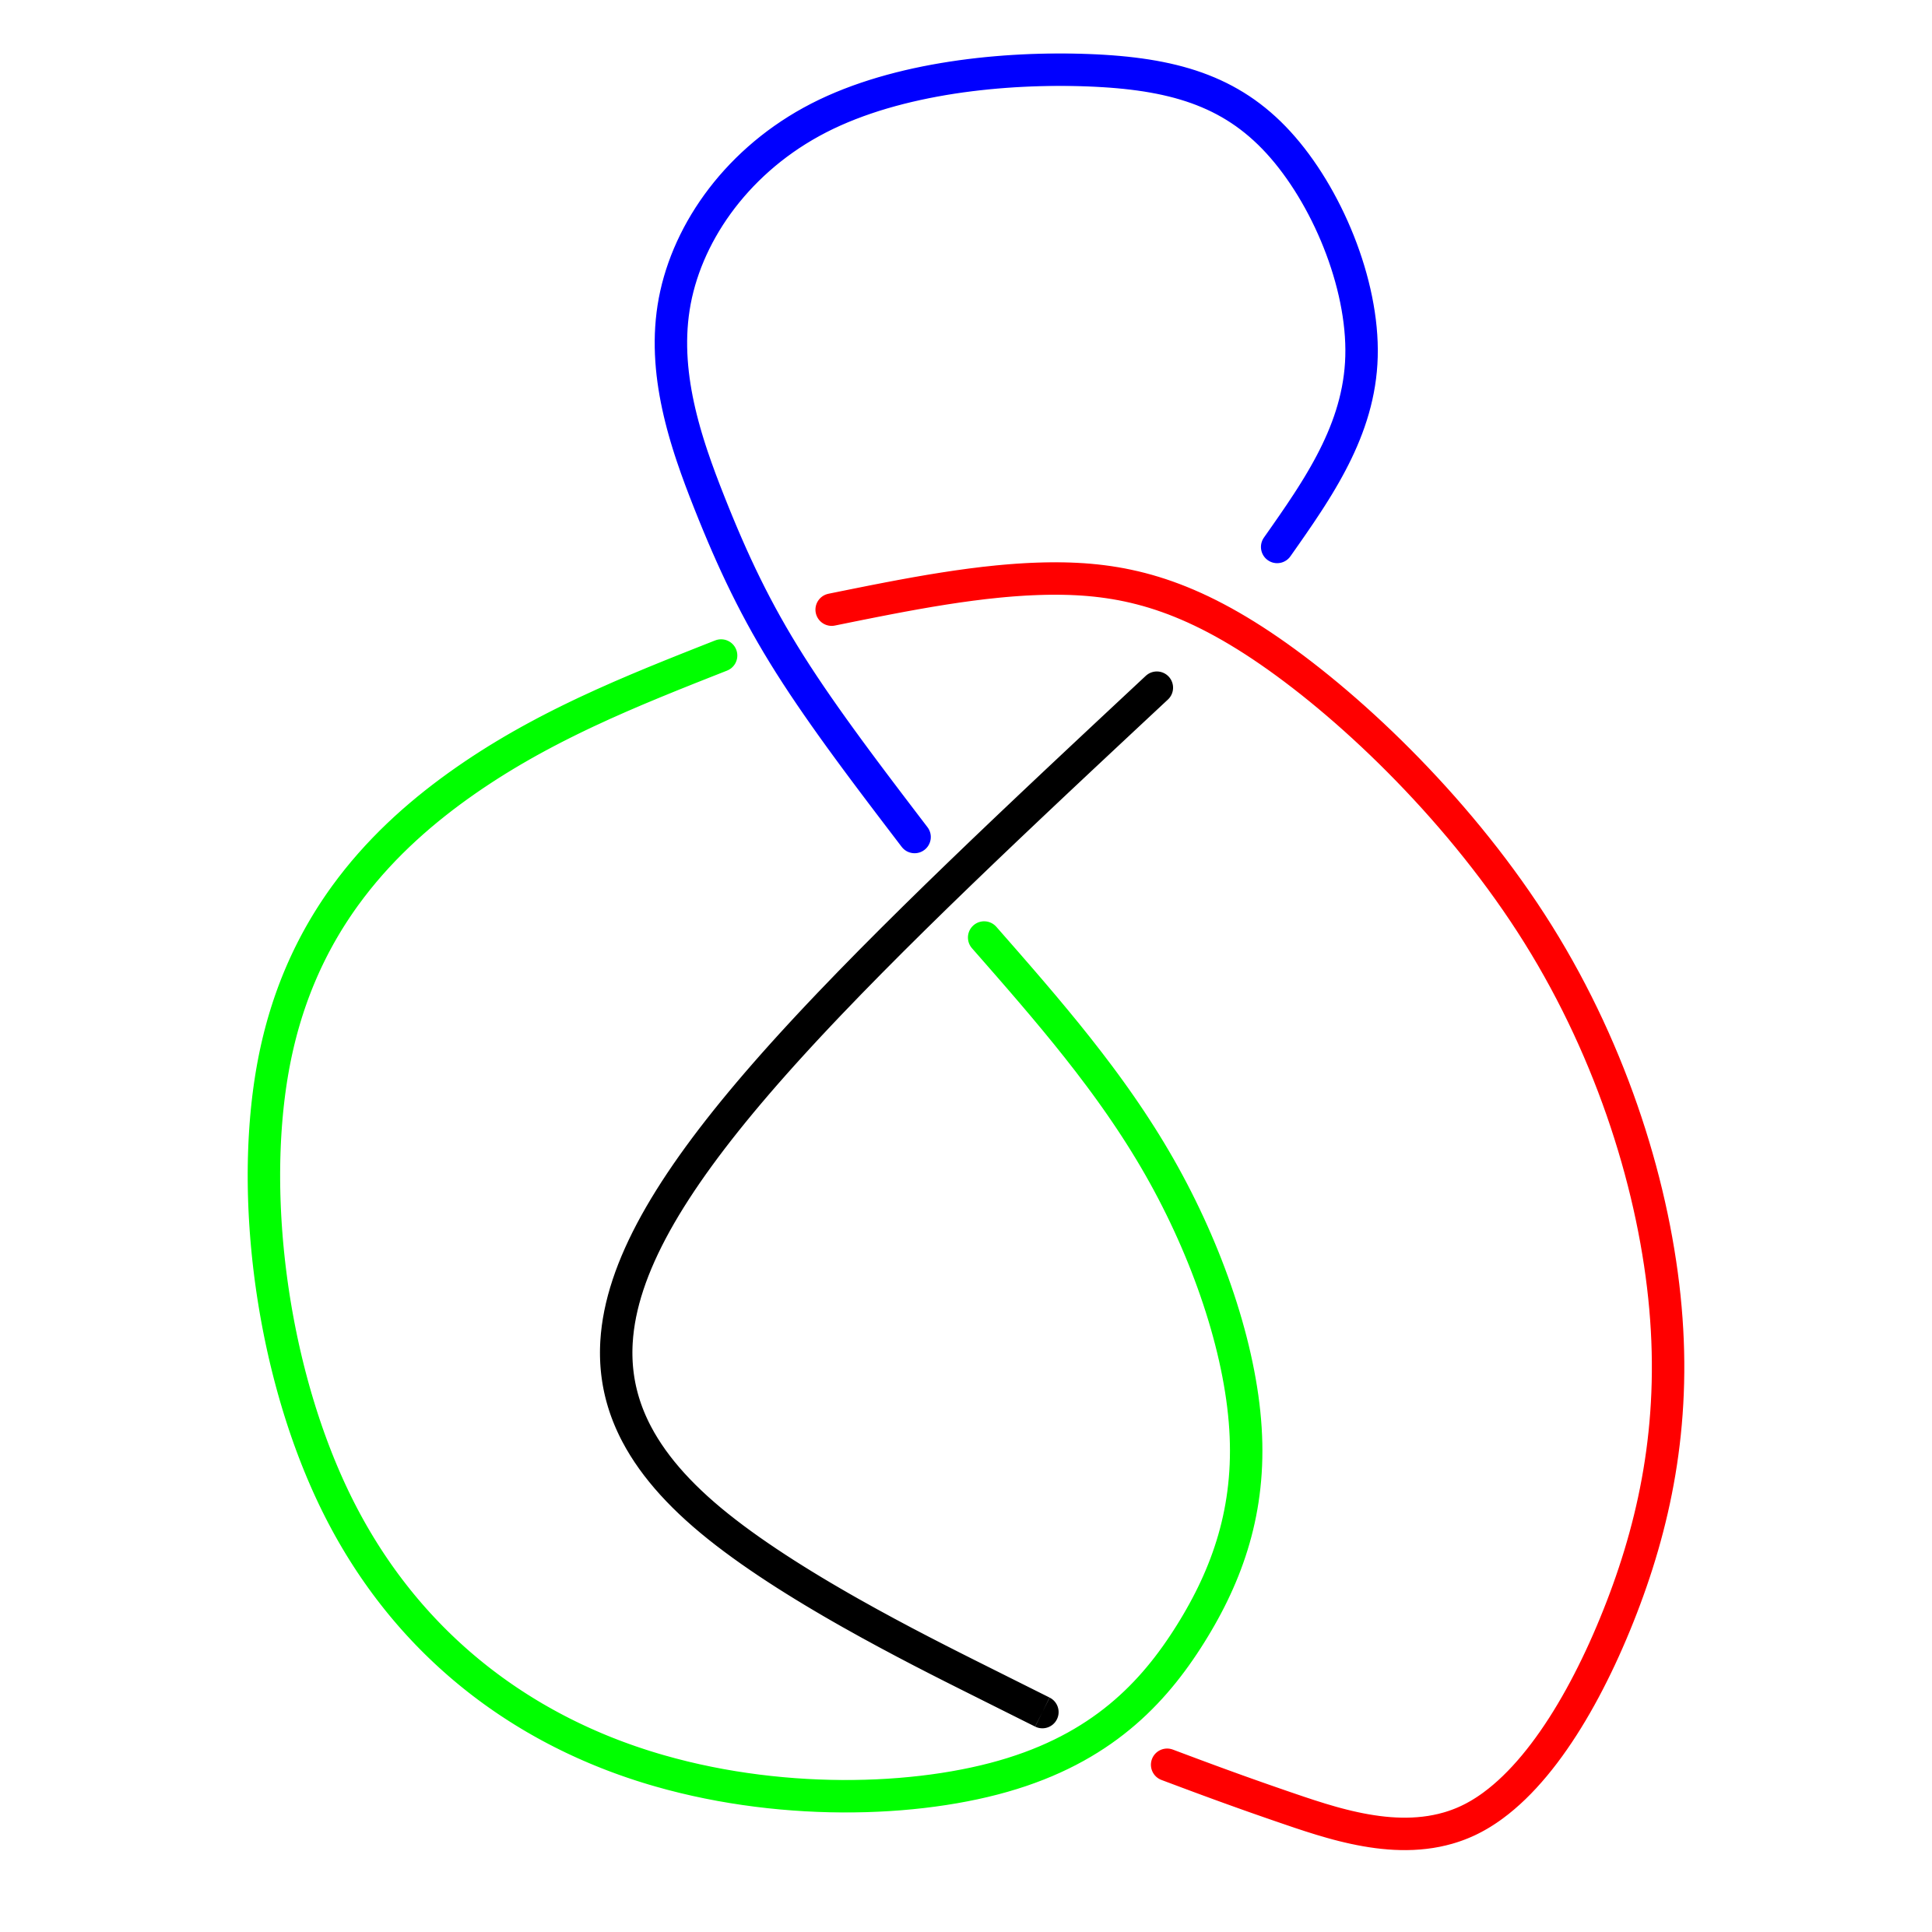
\includegraphics[width=0.5\linewidth]{picture/knotpict/knot-9}
	\caption{9th Combination}
\end{subfigure}
\qquad
\begin{subfigure}[b]{0.25\linewidth}
	\centering
	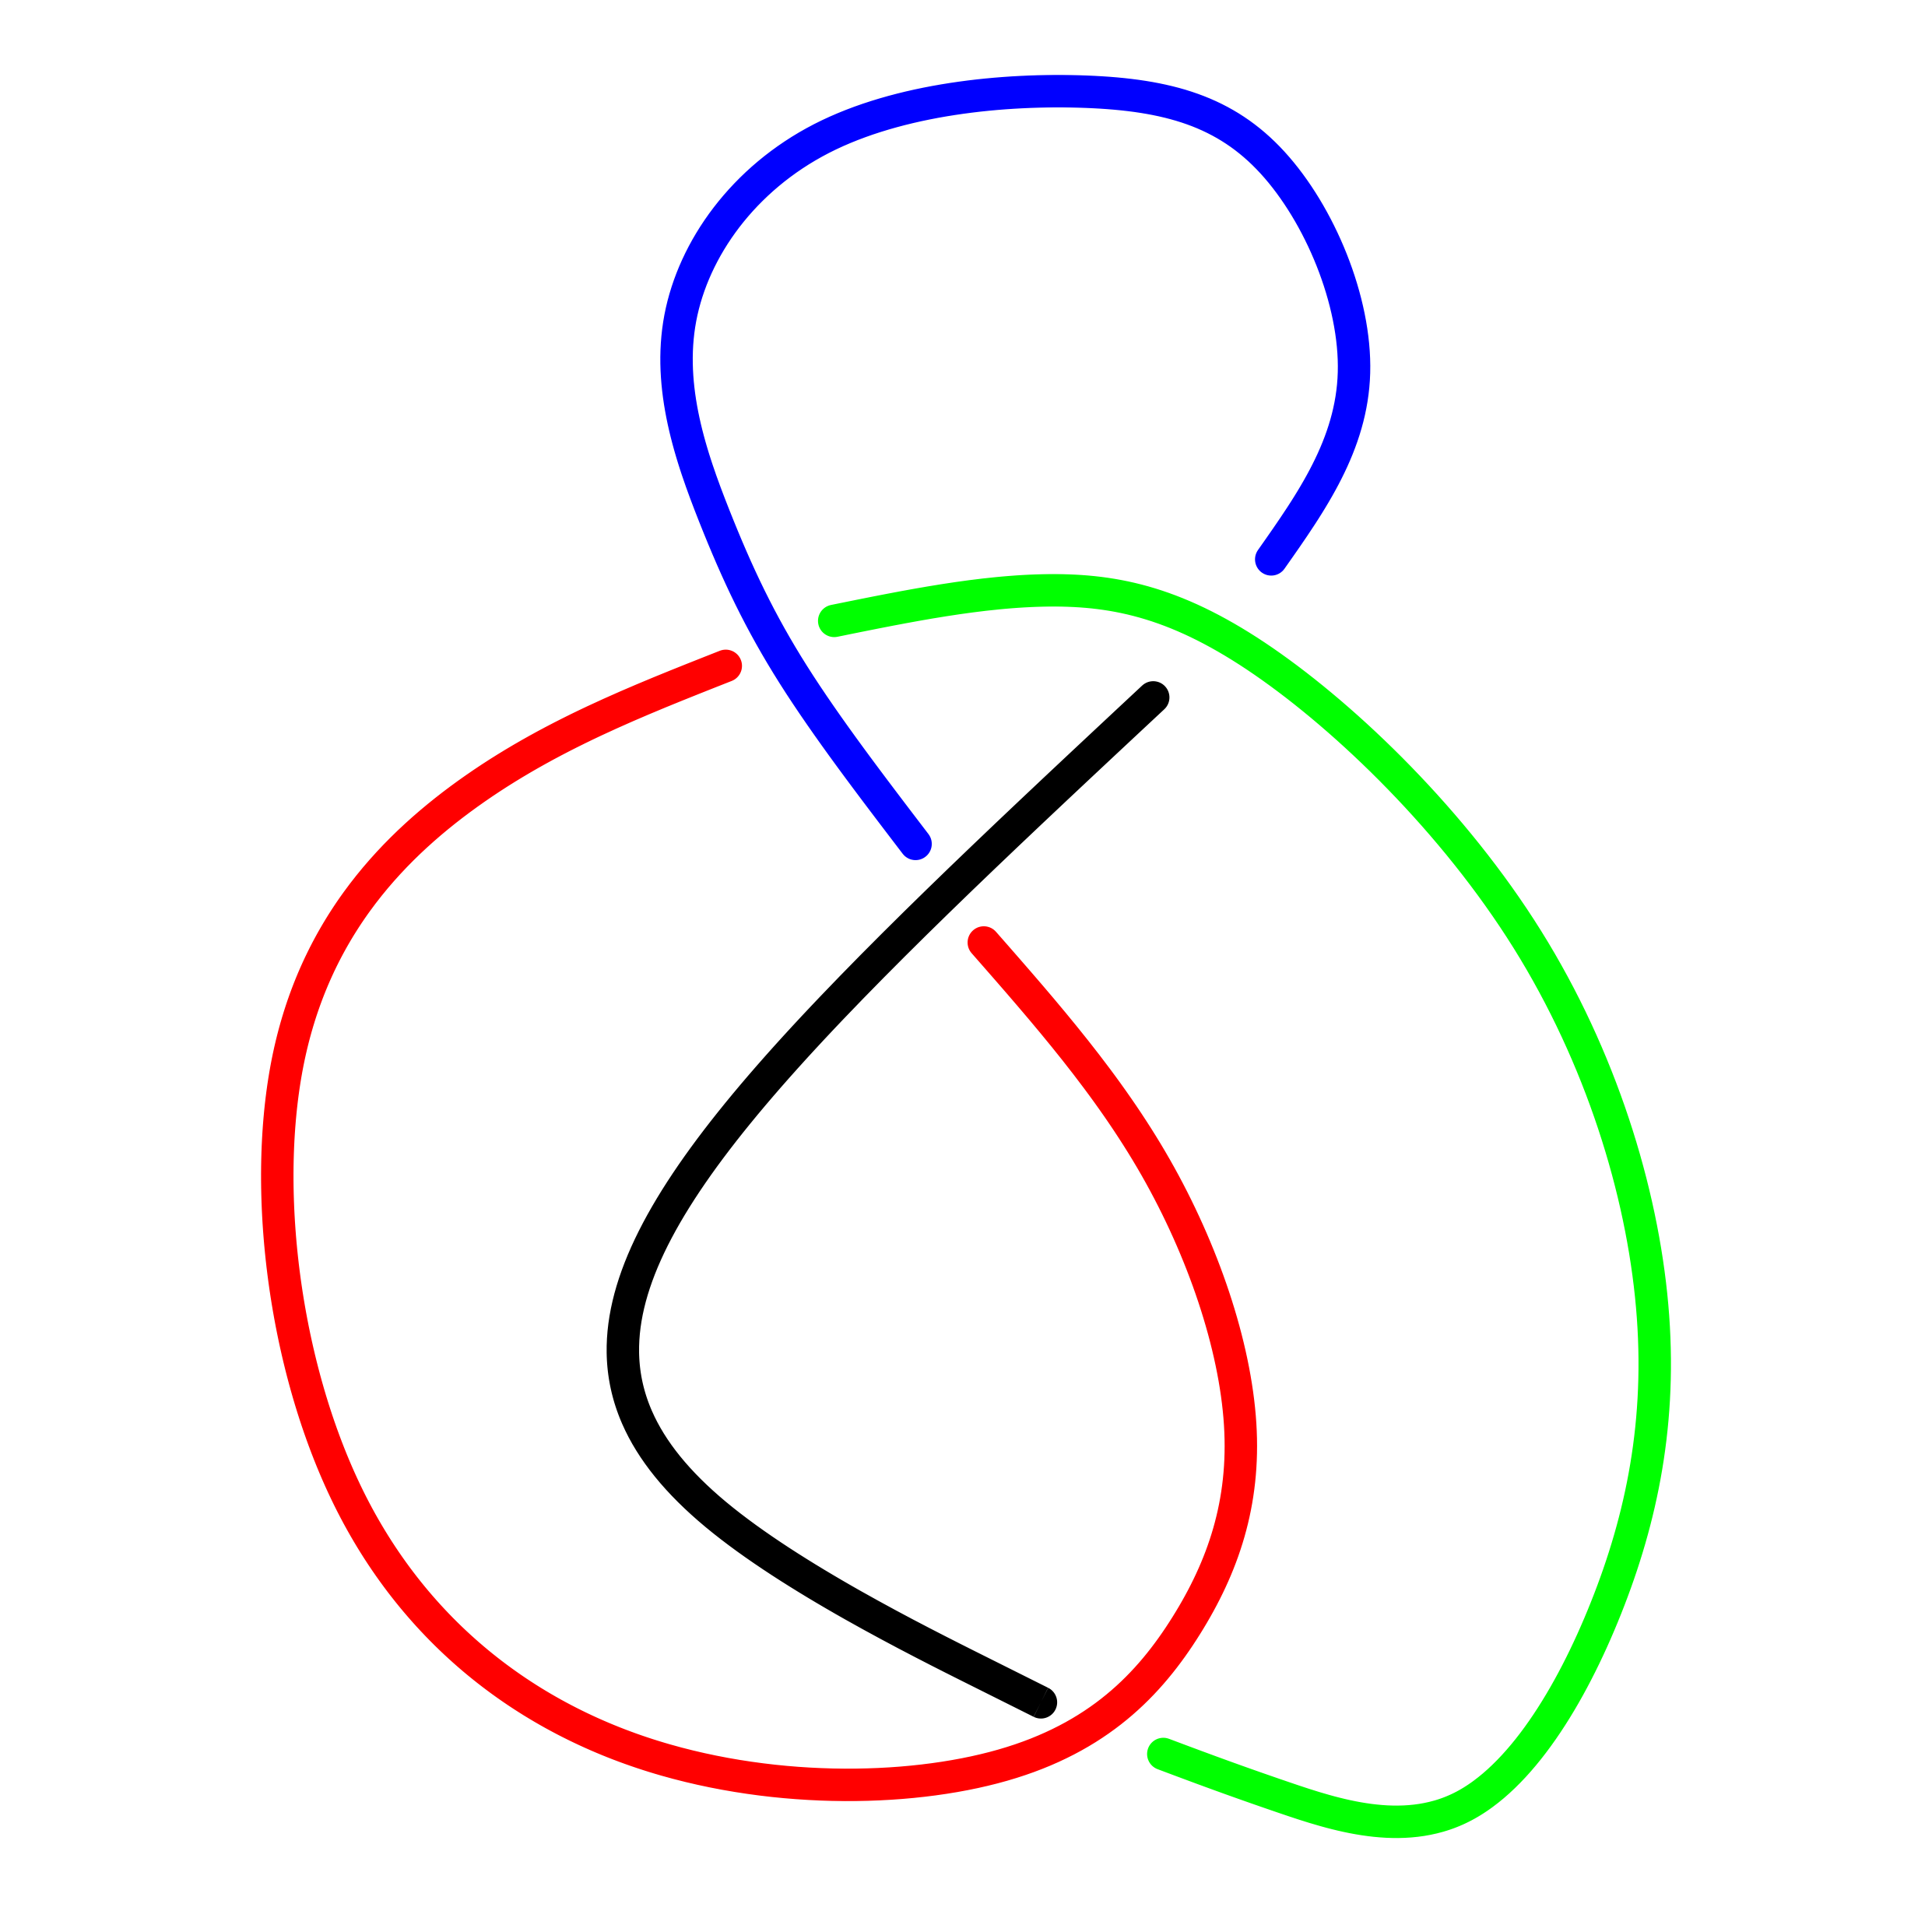
\includegraphics[width=0.5\linewidth]{picture/knotpict/knot-10}
	\caption{10th Combination}
\end{subfigure}
\qquad
\begin{subfigure}[b]{0.25\linewidth}
	\centering
	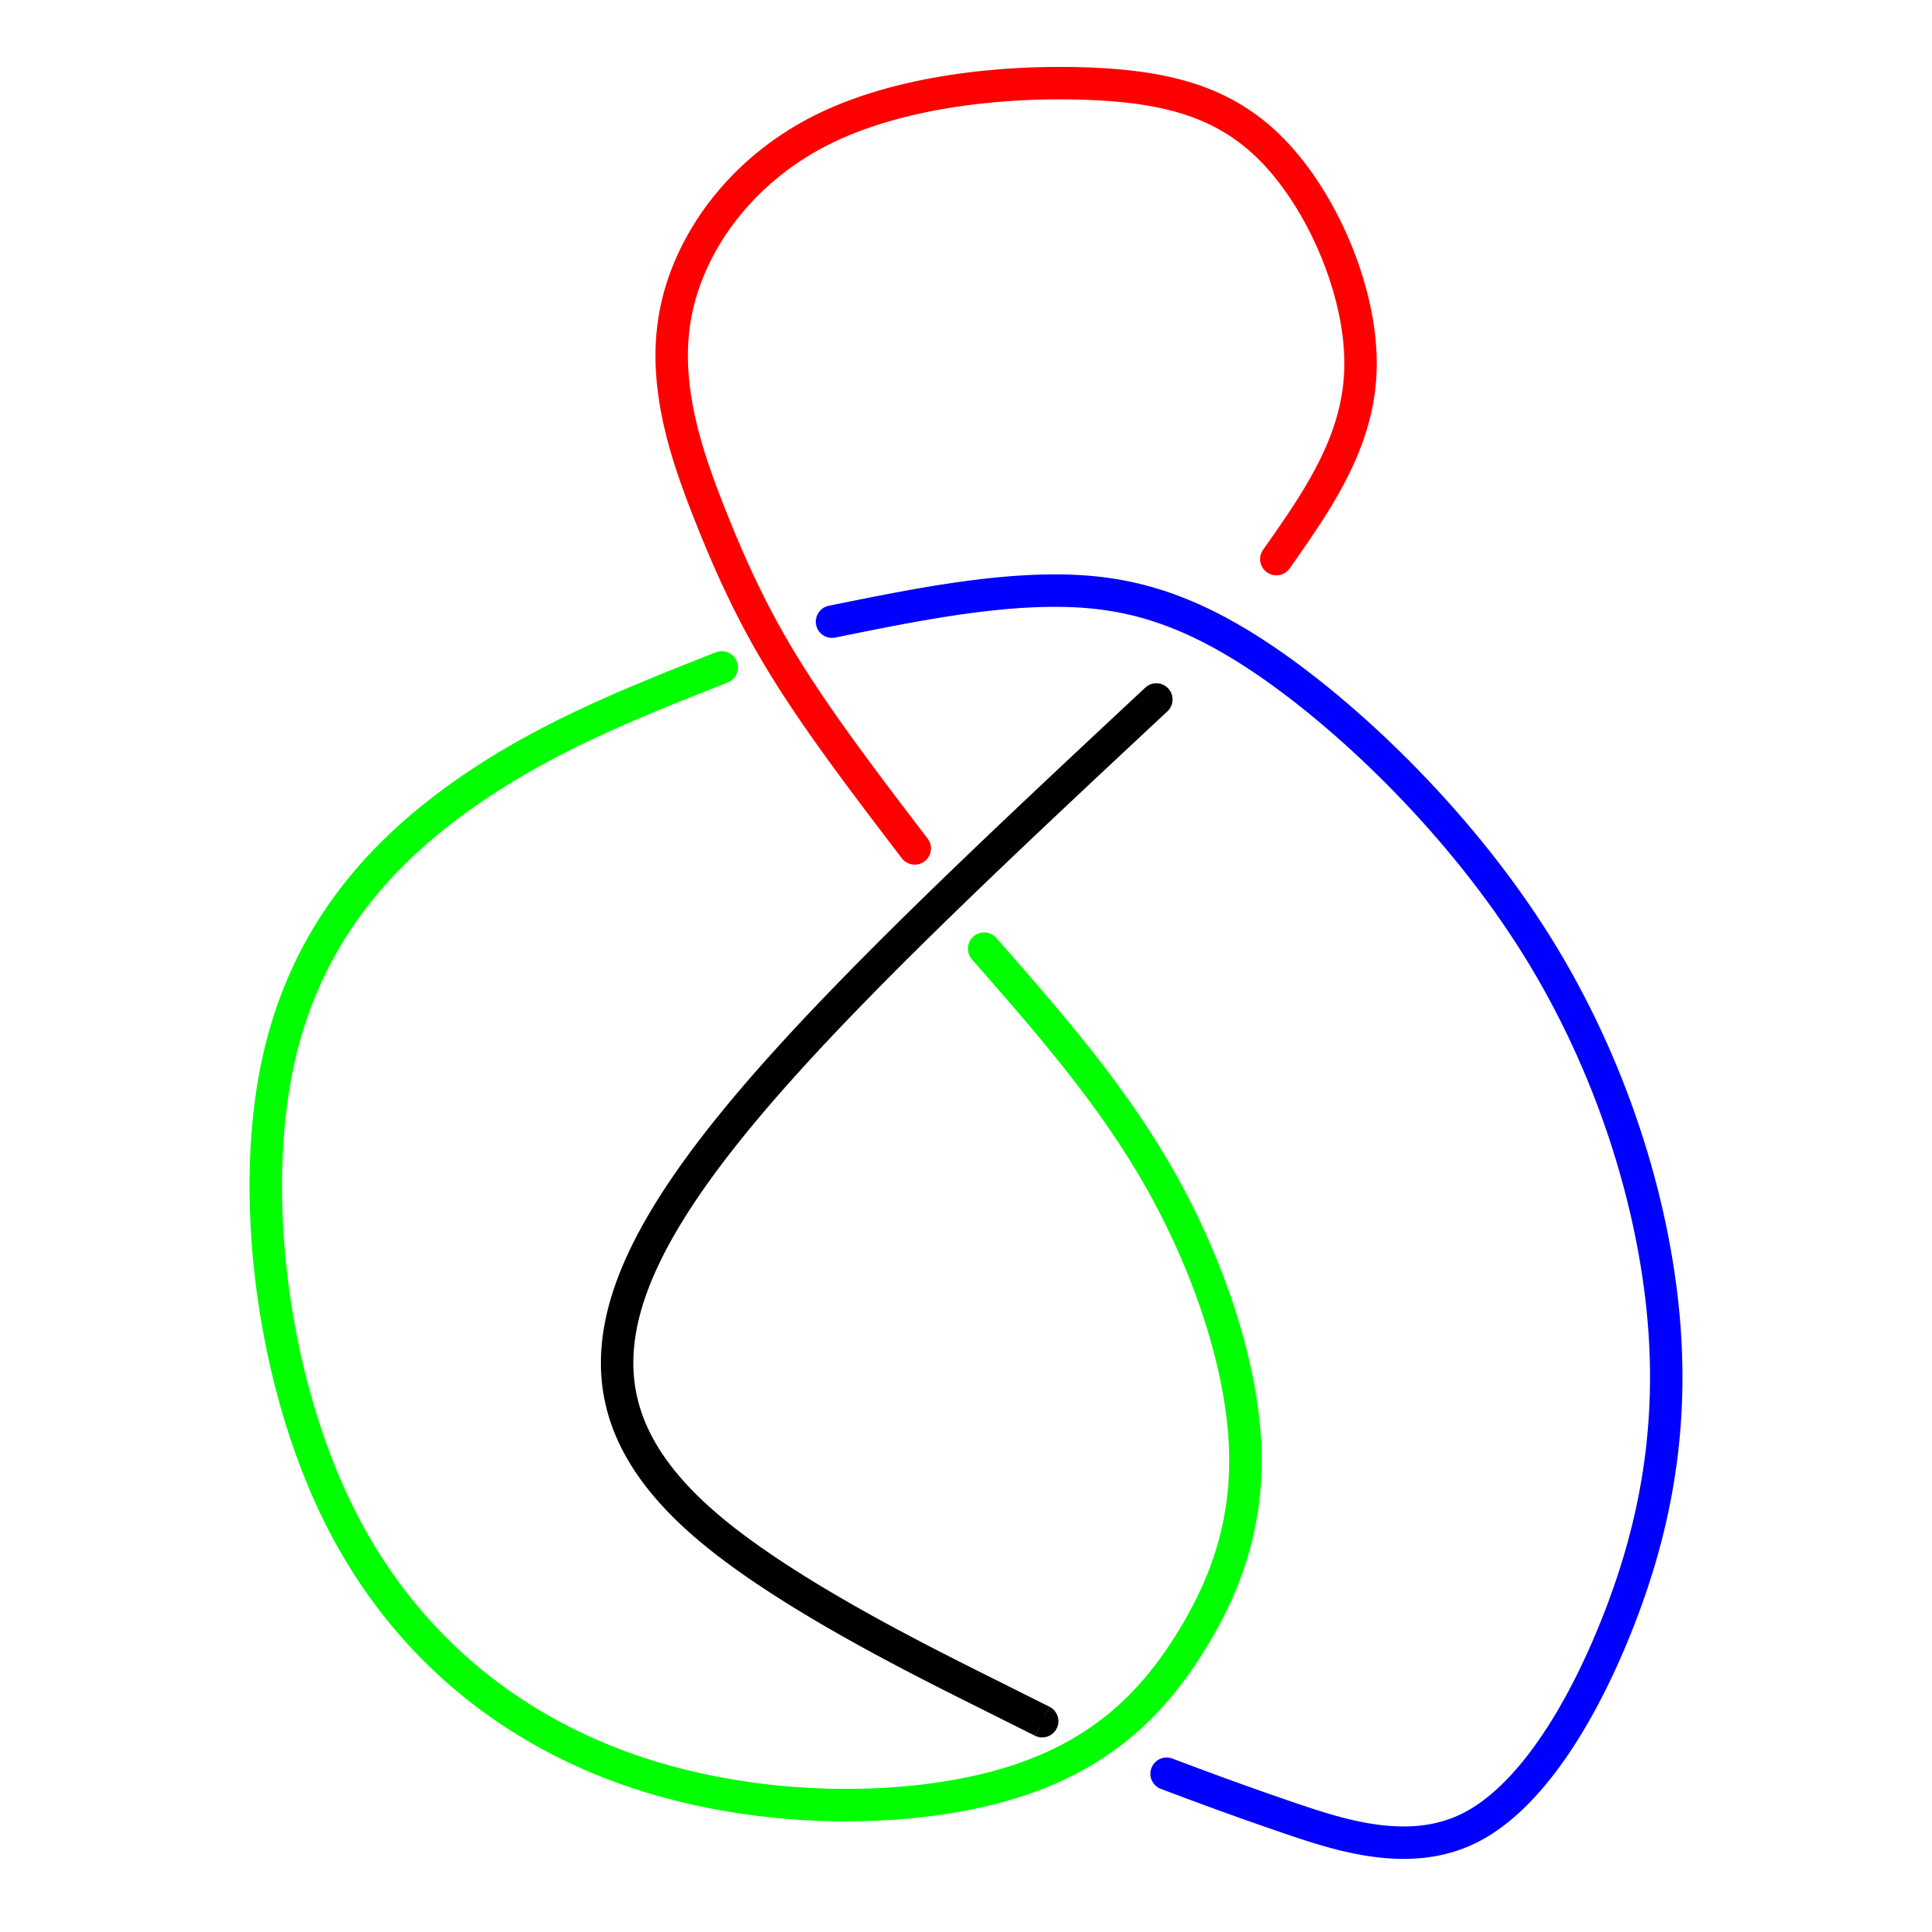
\includegraphics[width=0.5\linewidth]{picture/knotpict/knot-11}
	\caption{11th Combination}
\end{subfigure}
\qquad
\begin{subfigure}[b]{0.25\linewidth}
	\centering
	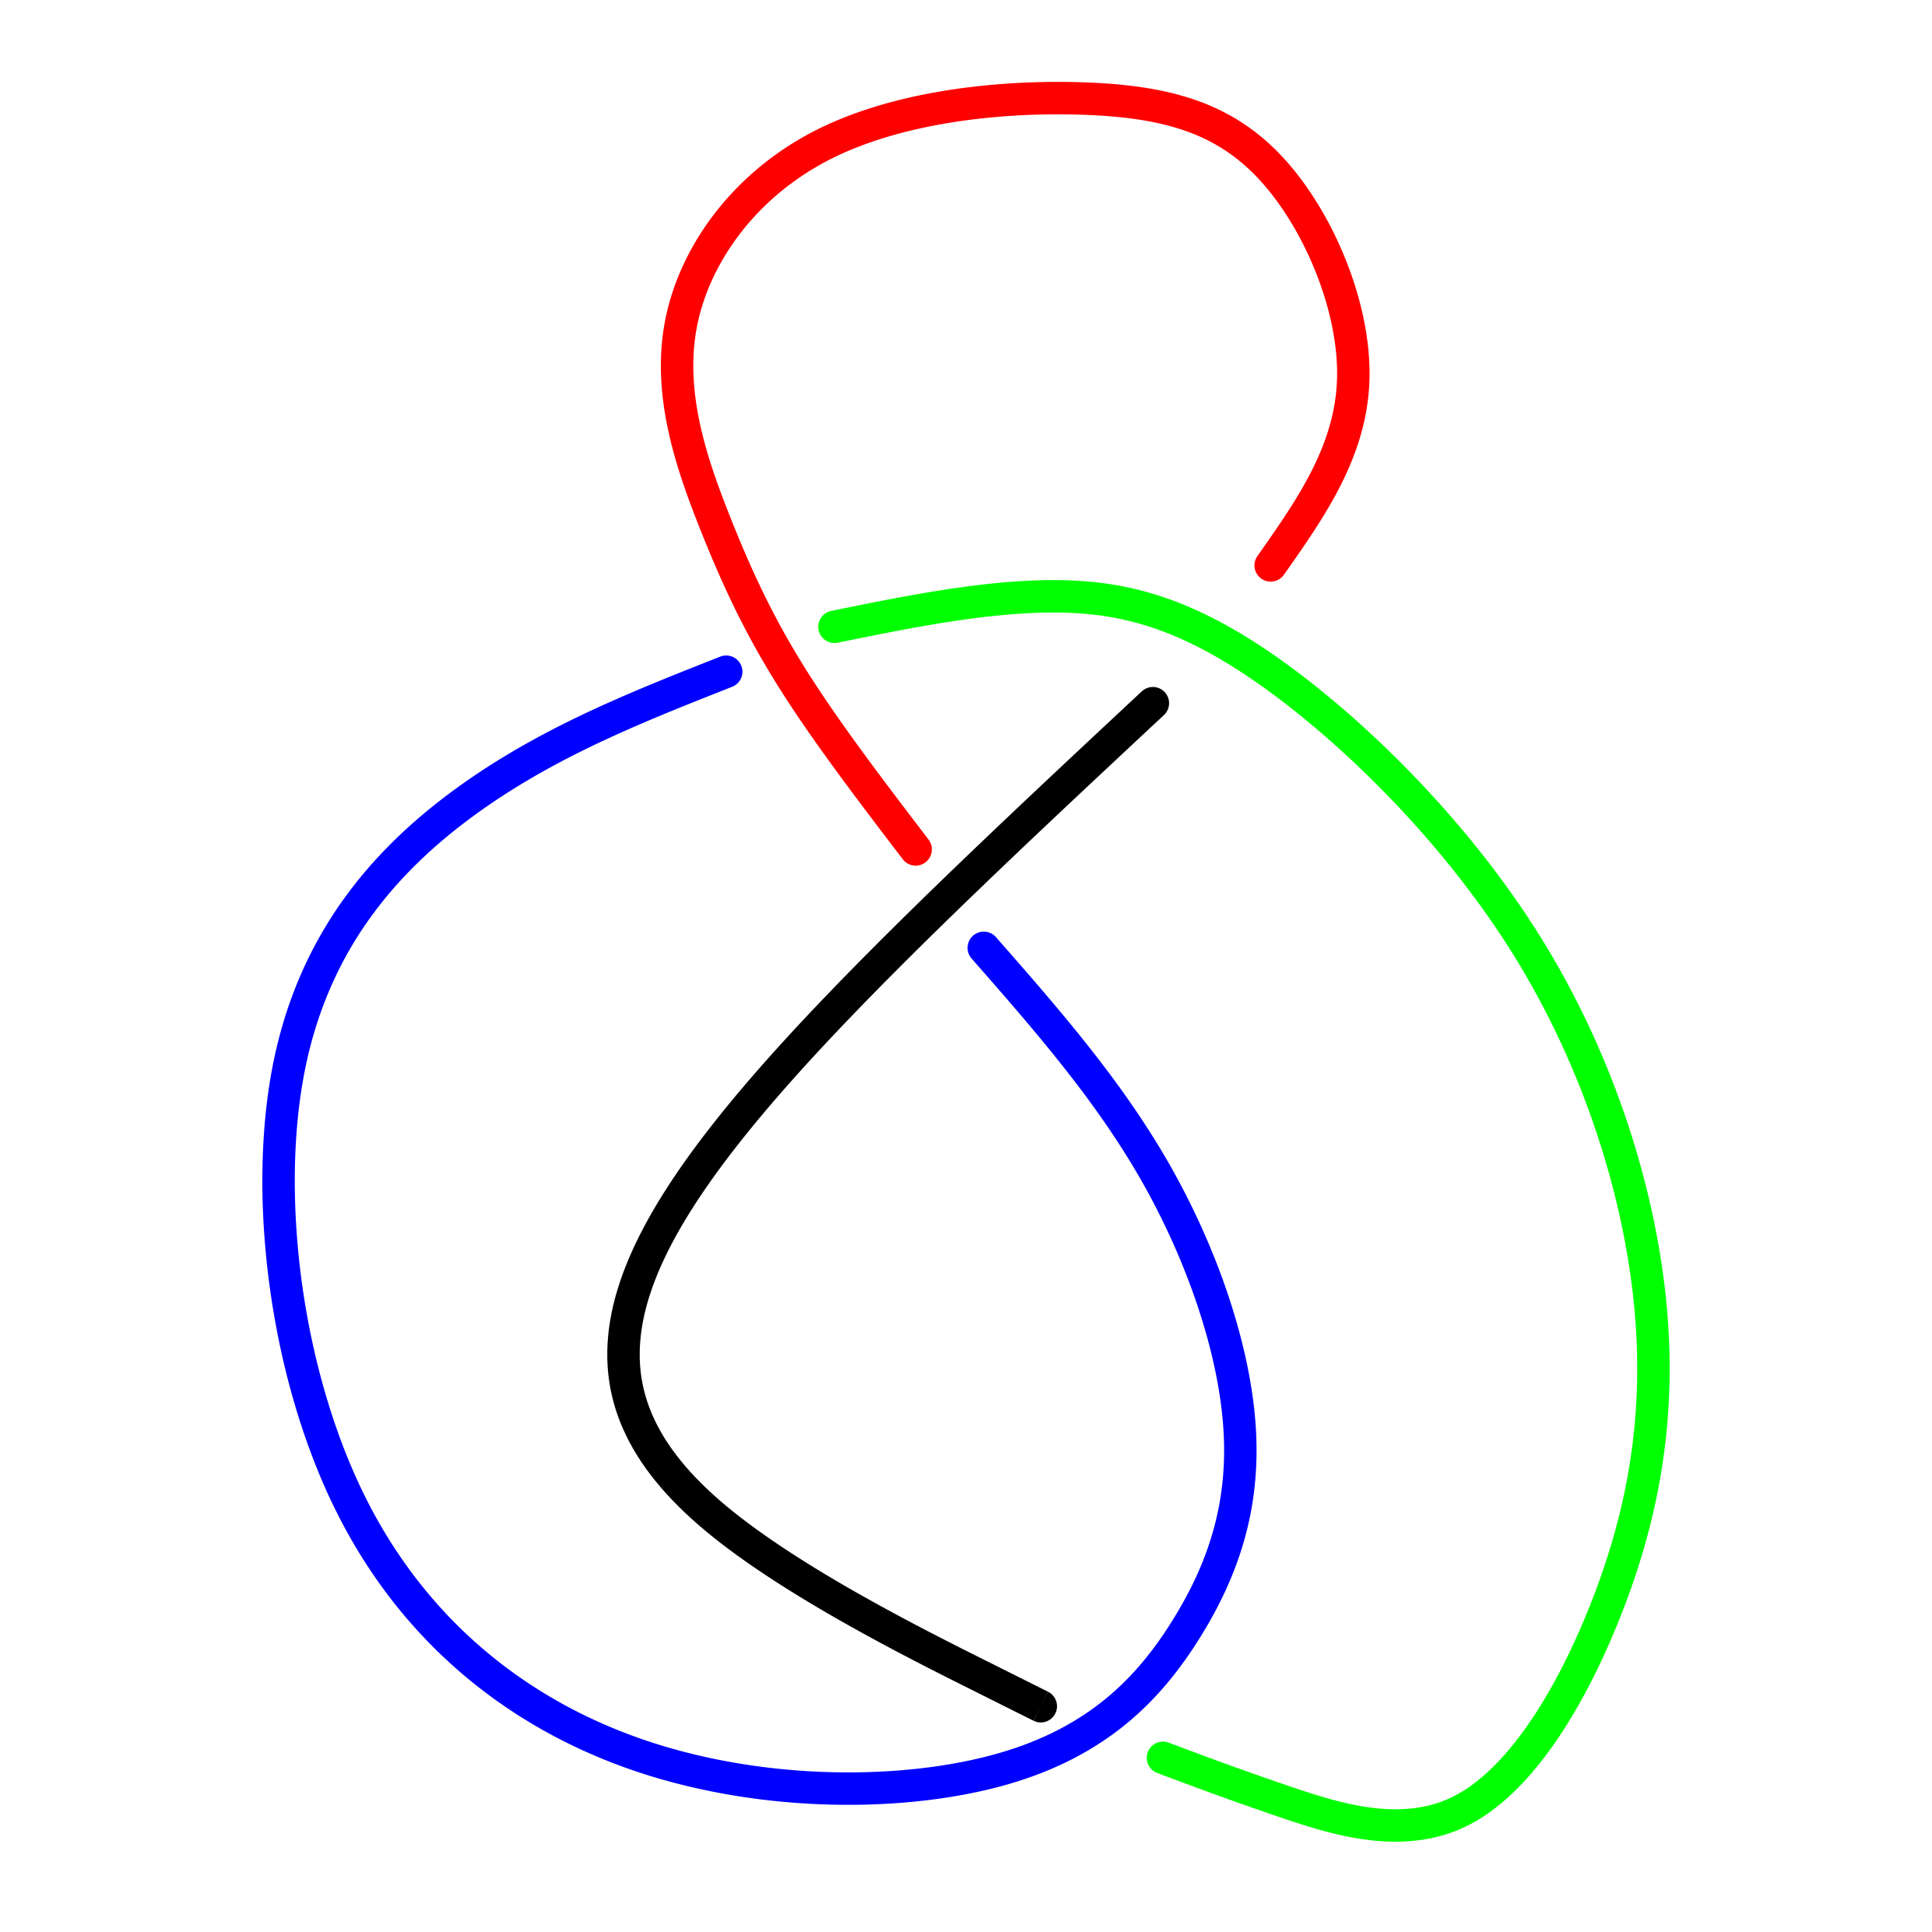
\includegraphics[width=0.5\linewidth]{picture/knotpict/knot-12}
	\caption{12th Combination}
\end{subfigure}
\qquad
\begin{subfigure}[b]{0.25\linewidth}
	\centering
	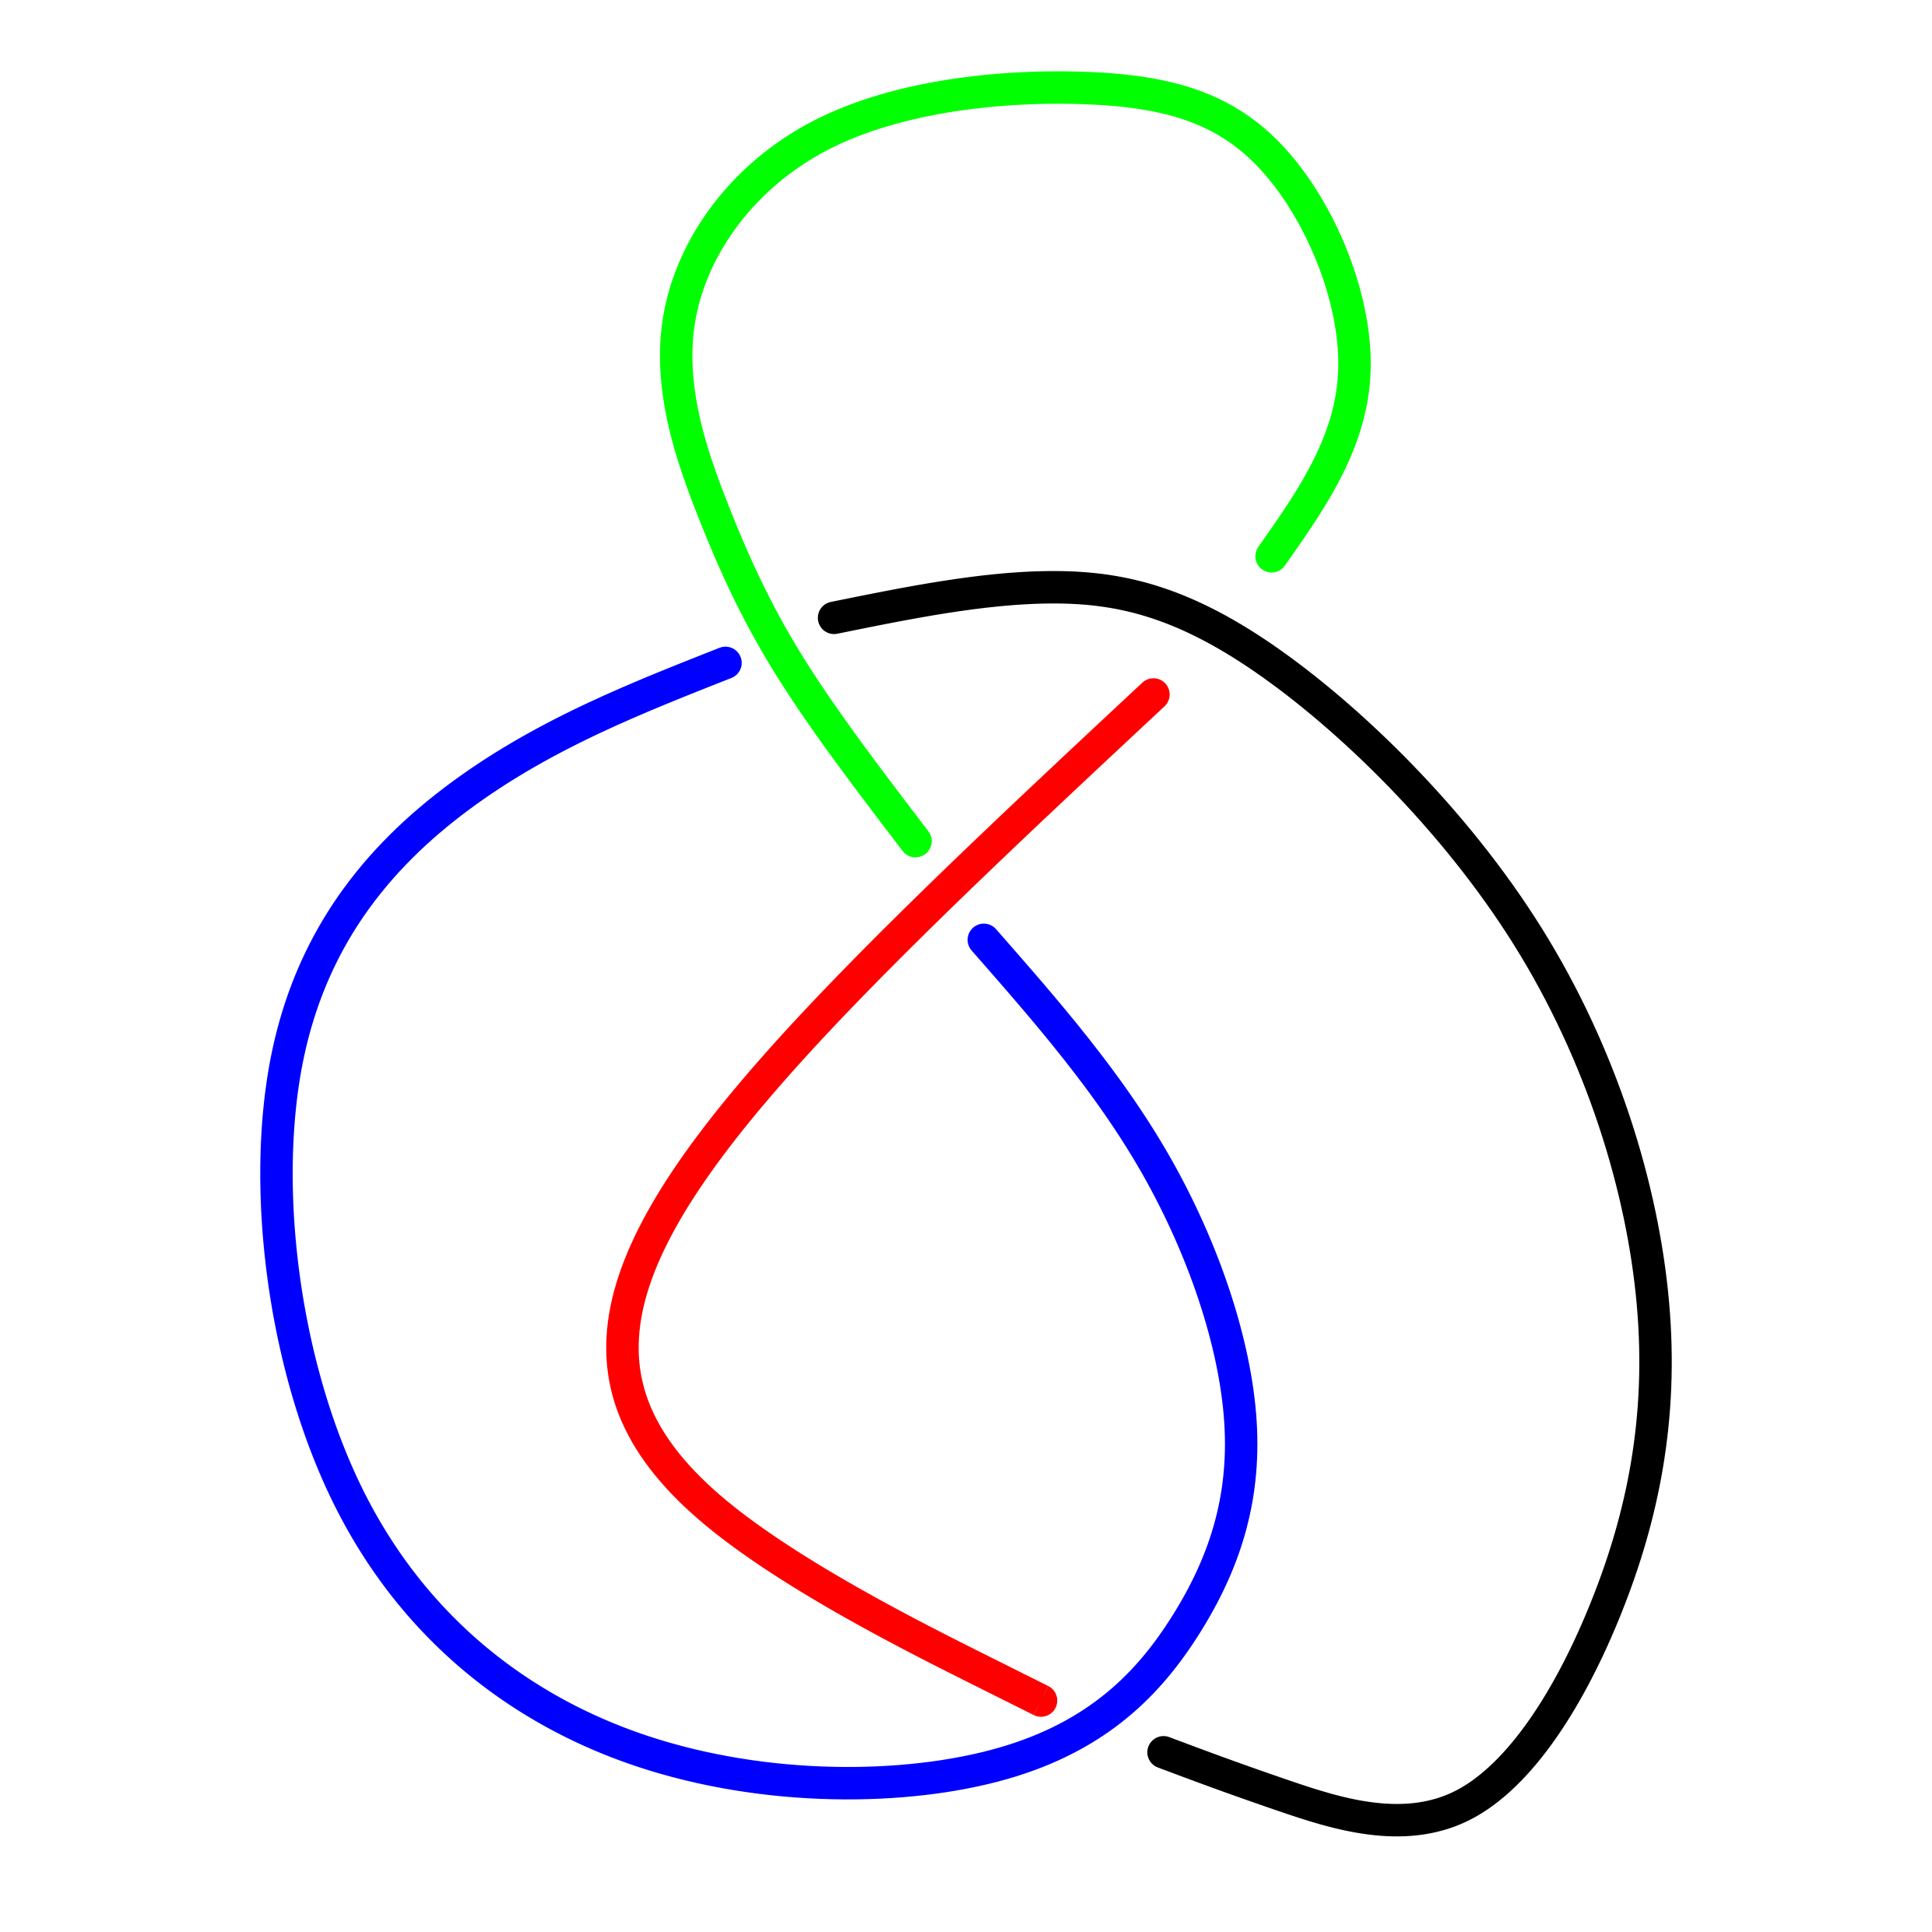
\includegraphics[width=0.5\linewidth]{picture/knotpict/knot-13}
	\caption{13th Combination}
\end{subfigure}
\qquad
\begin{subfigure}[b]{0.25\linewidth}
	\centering
	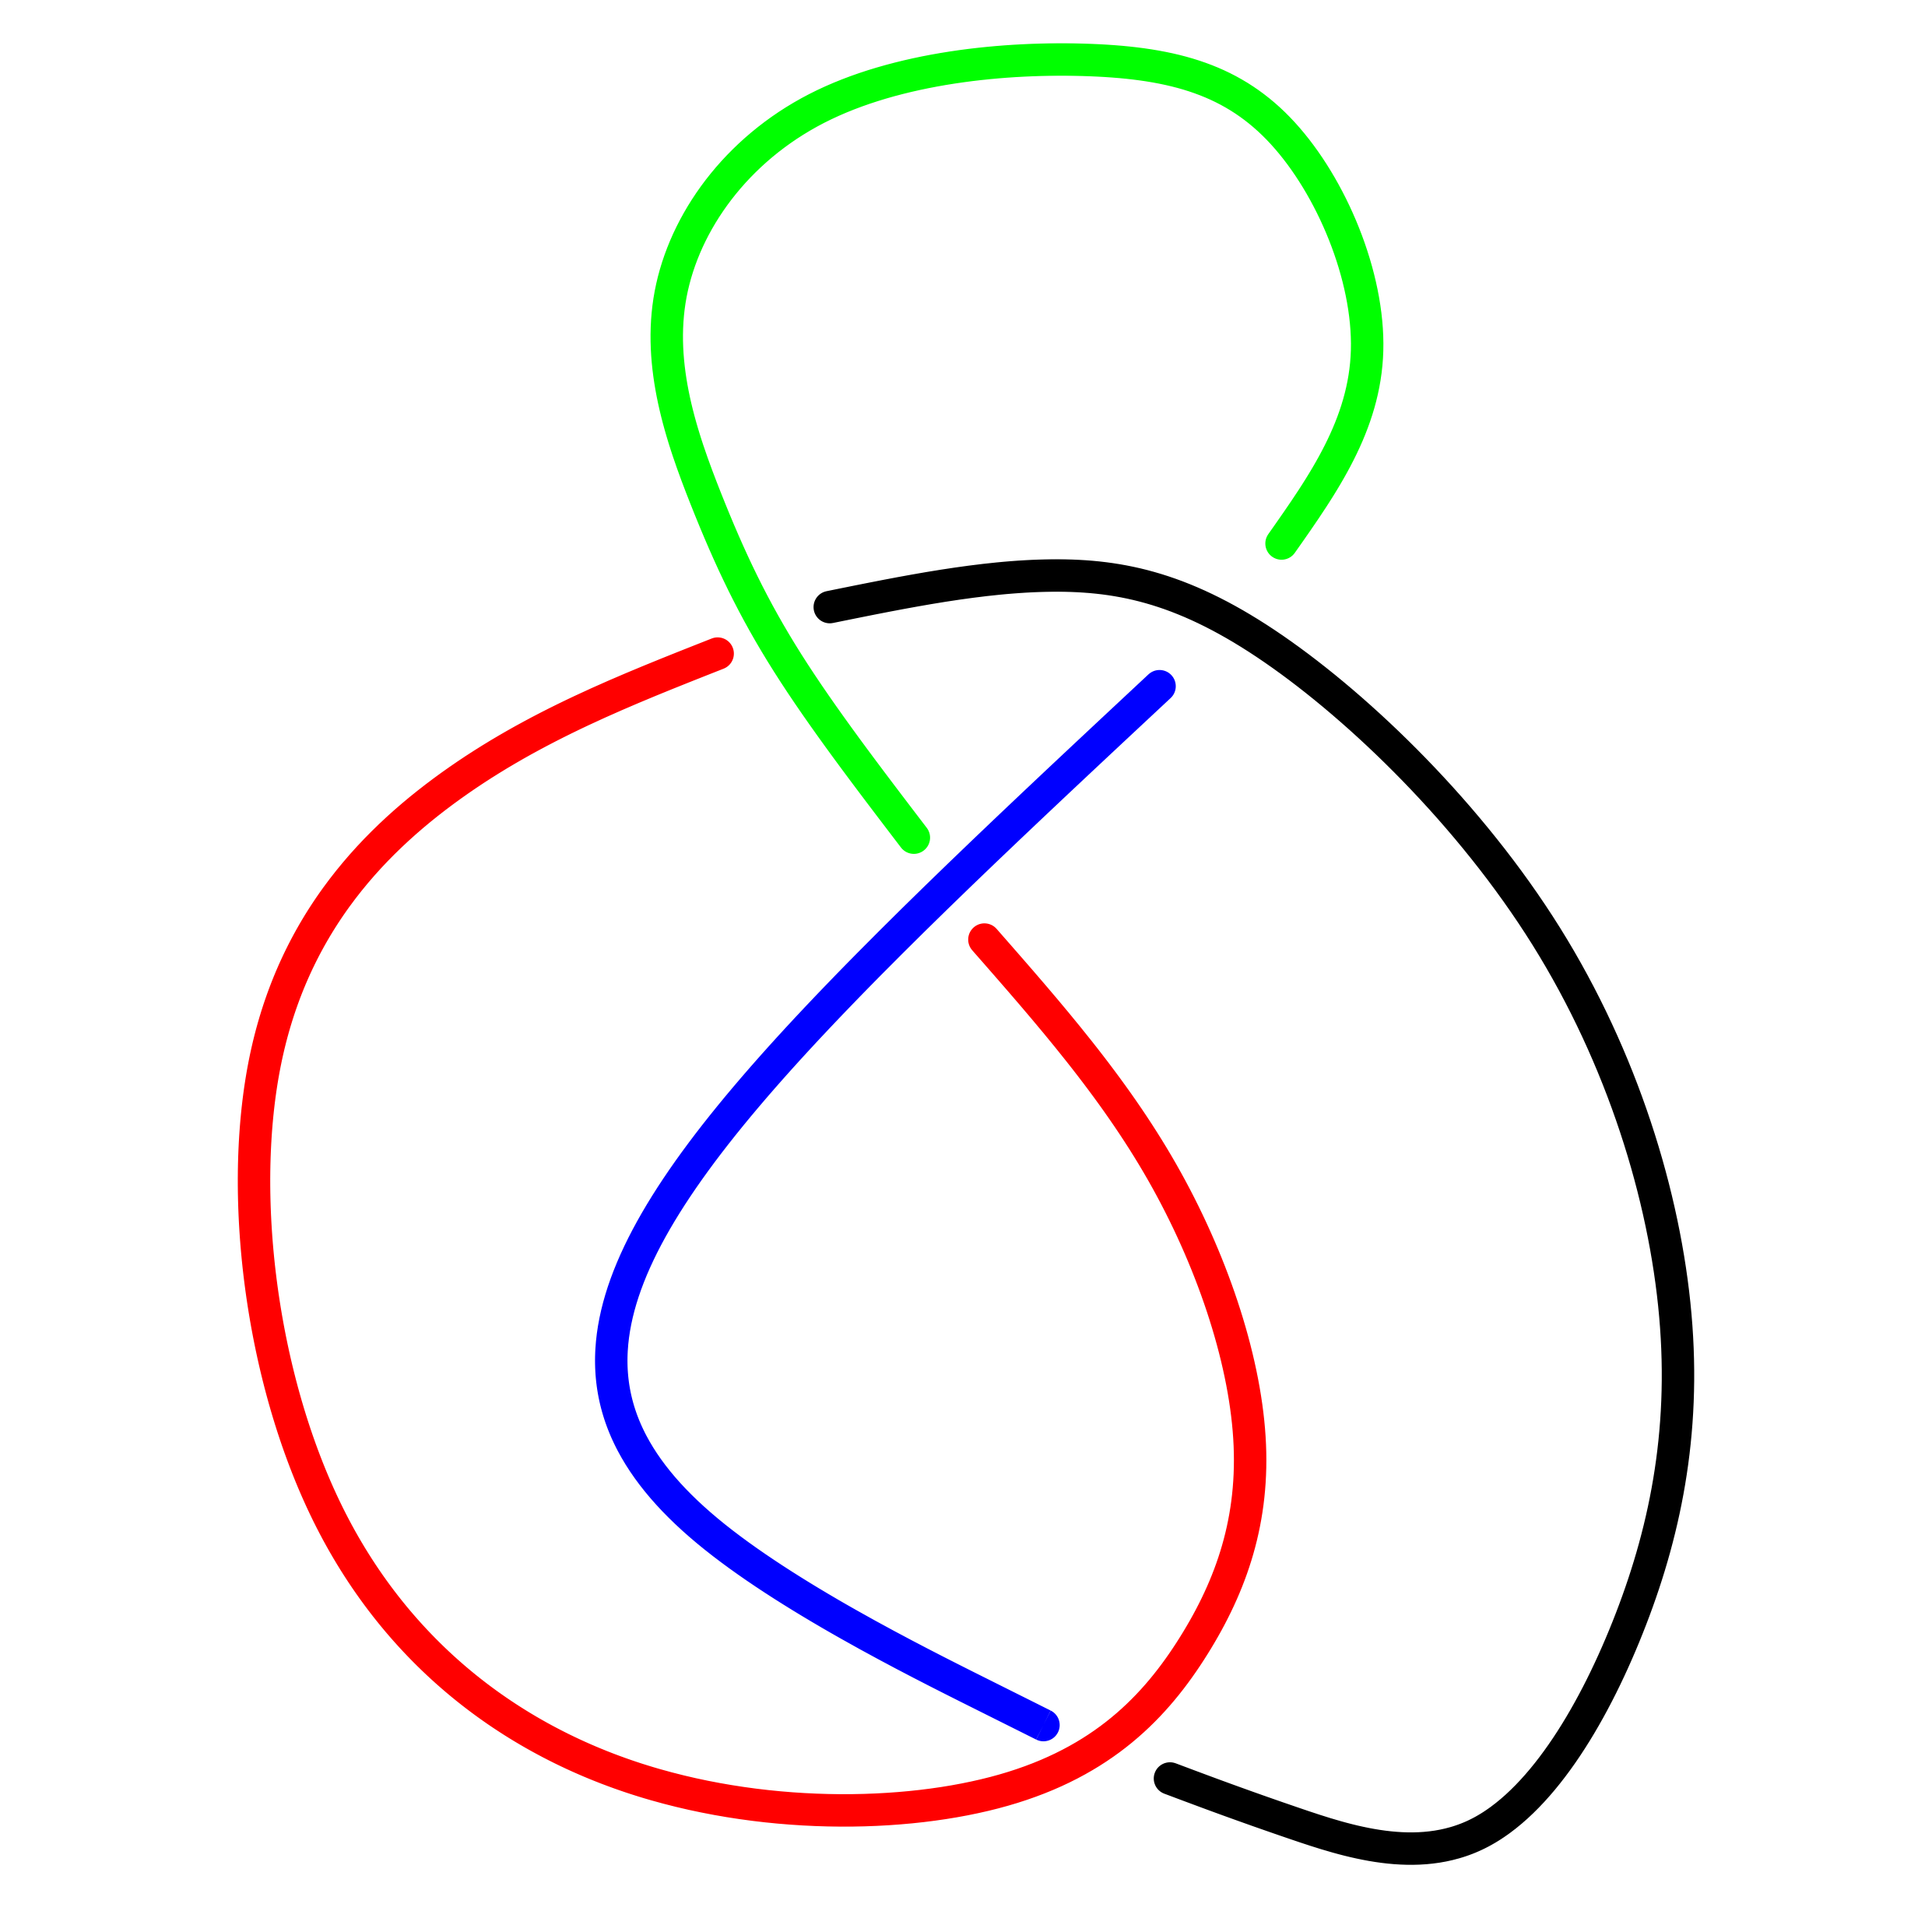
\includegraphics[width=0.5\linewidth]{picture/knotpict/knot-14}
	\caption{14th Combination}
\end{subfigure}
\qquad
\begin{subfigure}[b]{0.25\linewidth}
	\centering
	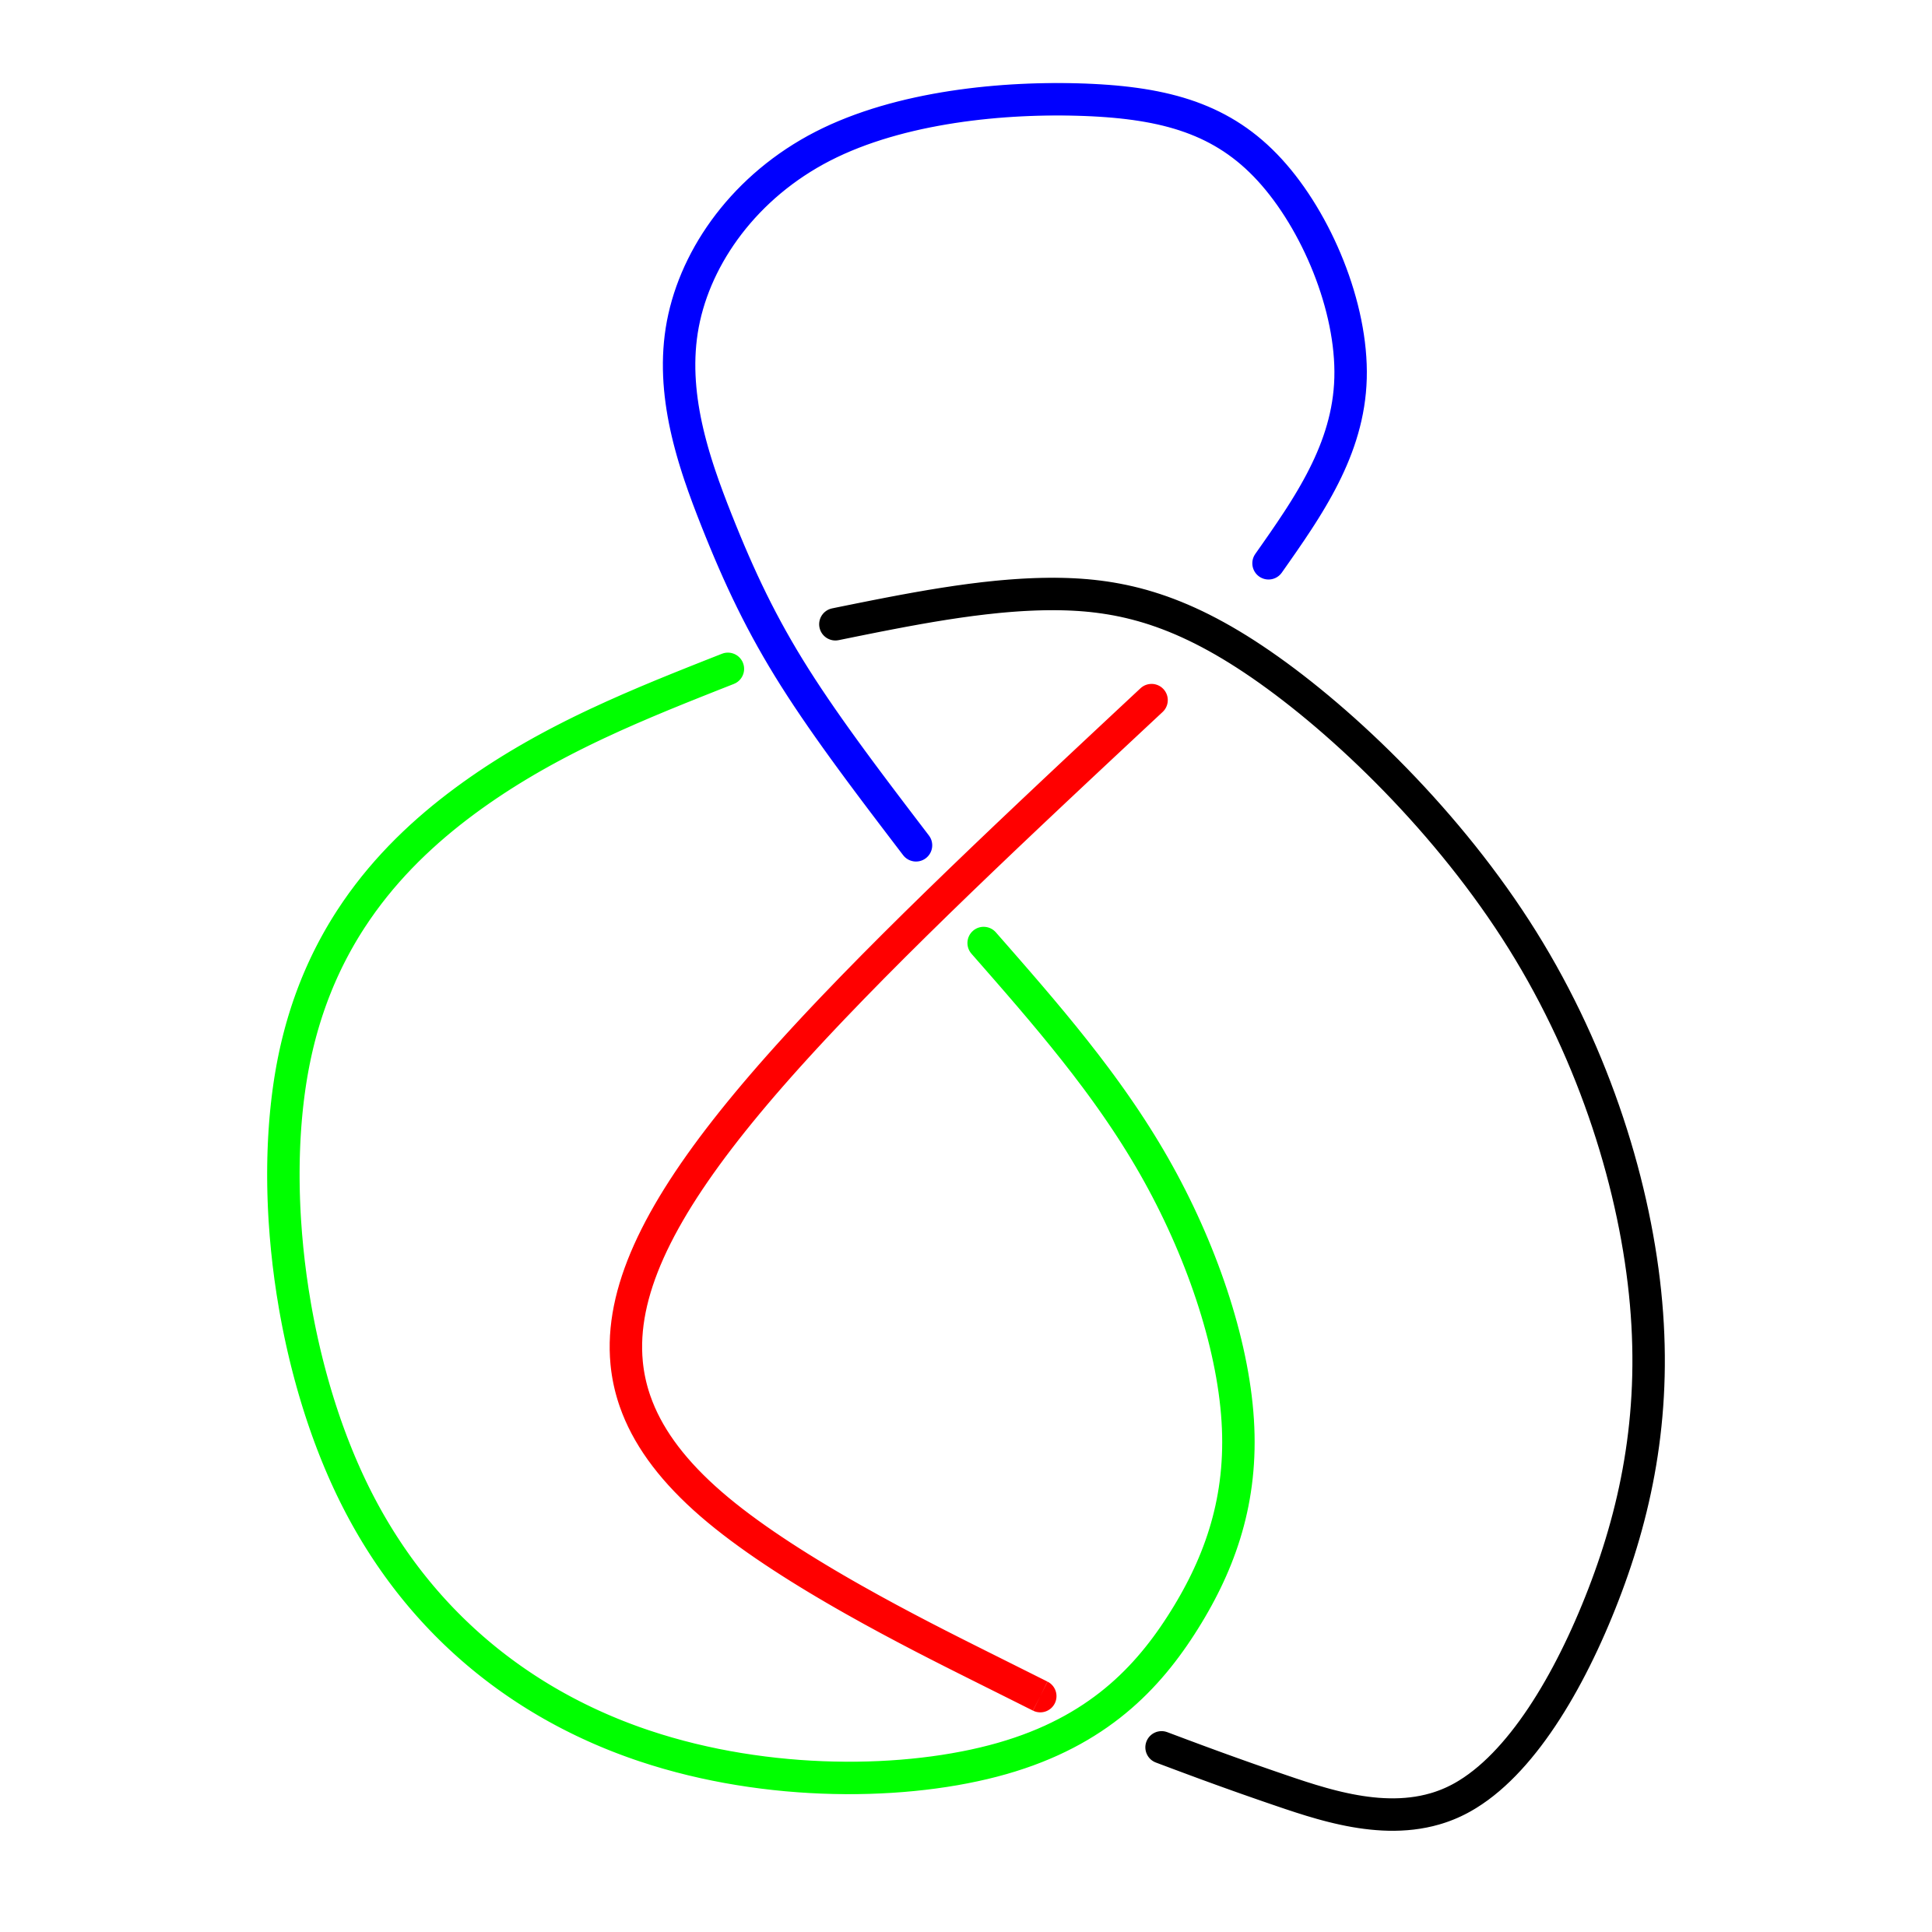
\includegraphics[width=0.5\linewidth]{picture/knotpict/knot-15}
	\caption{15th Combination}
\end{subfigure}
\qquad
\begin{subfigure}[b]{0.25\linewidth}
	\centering
	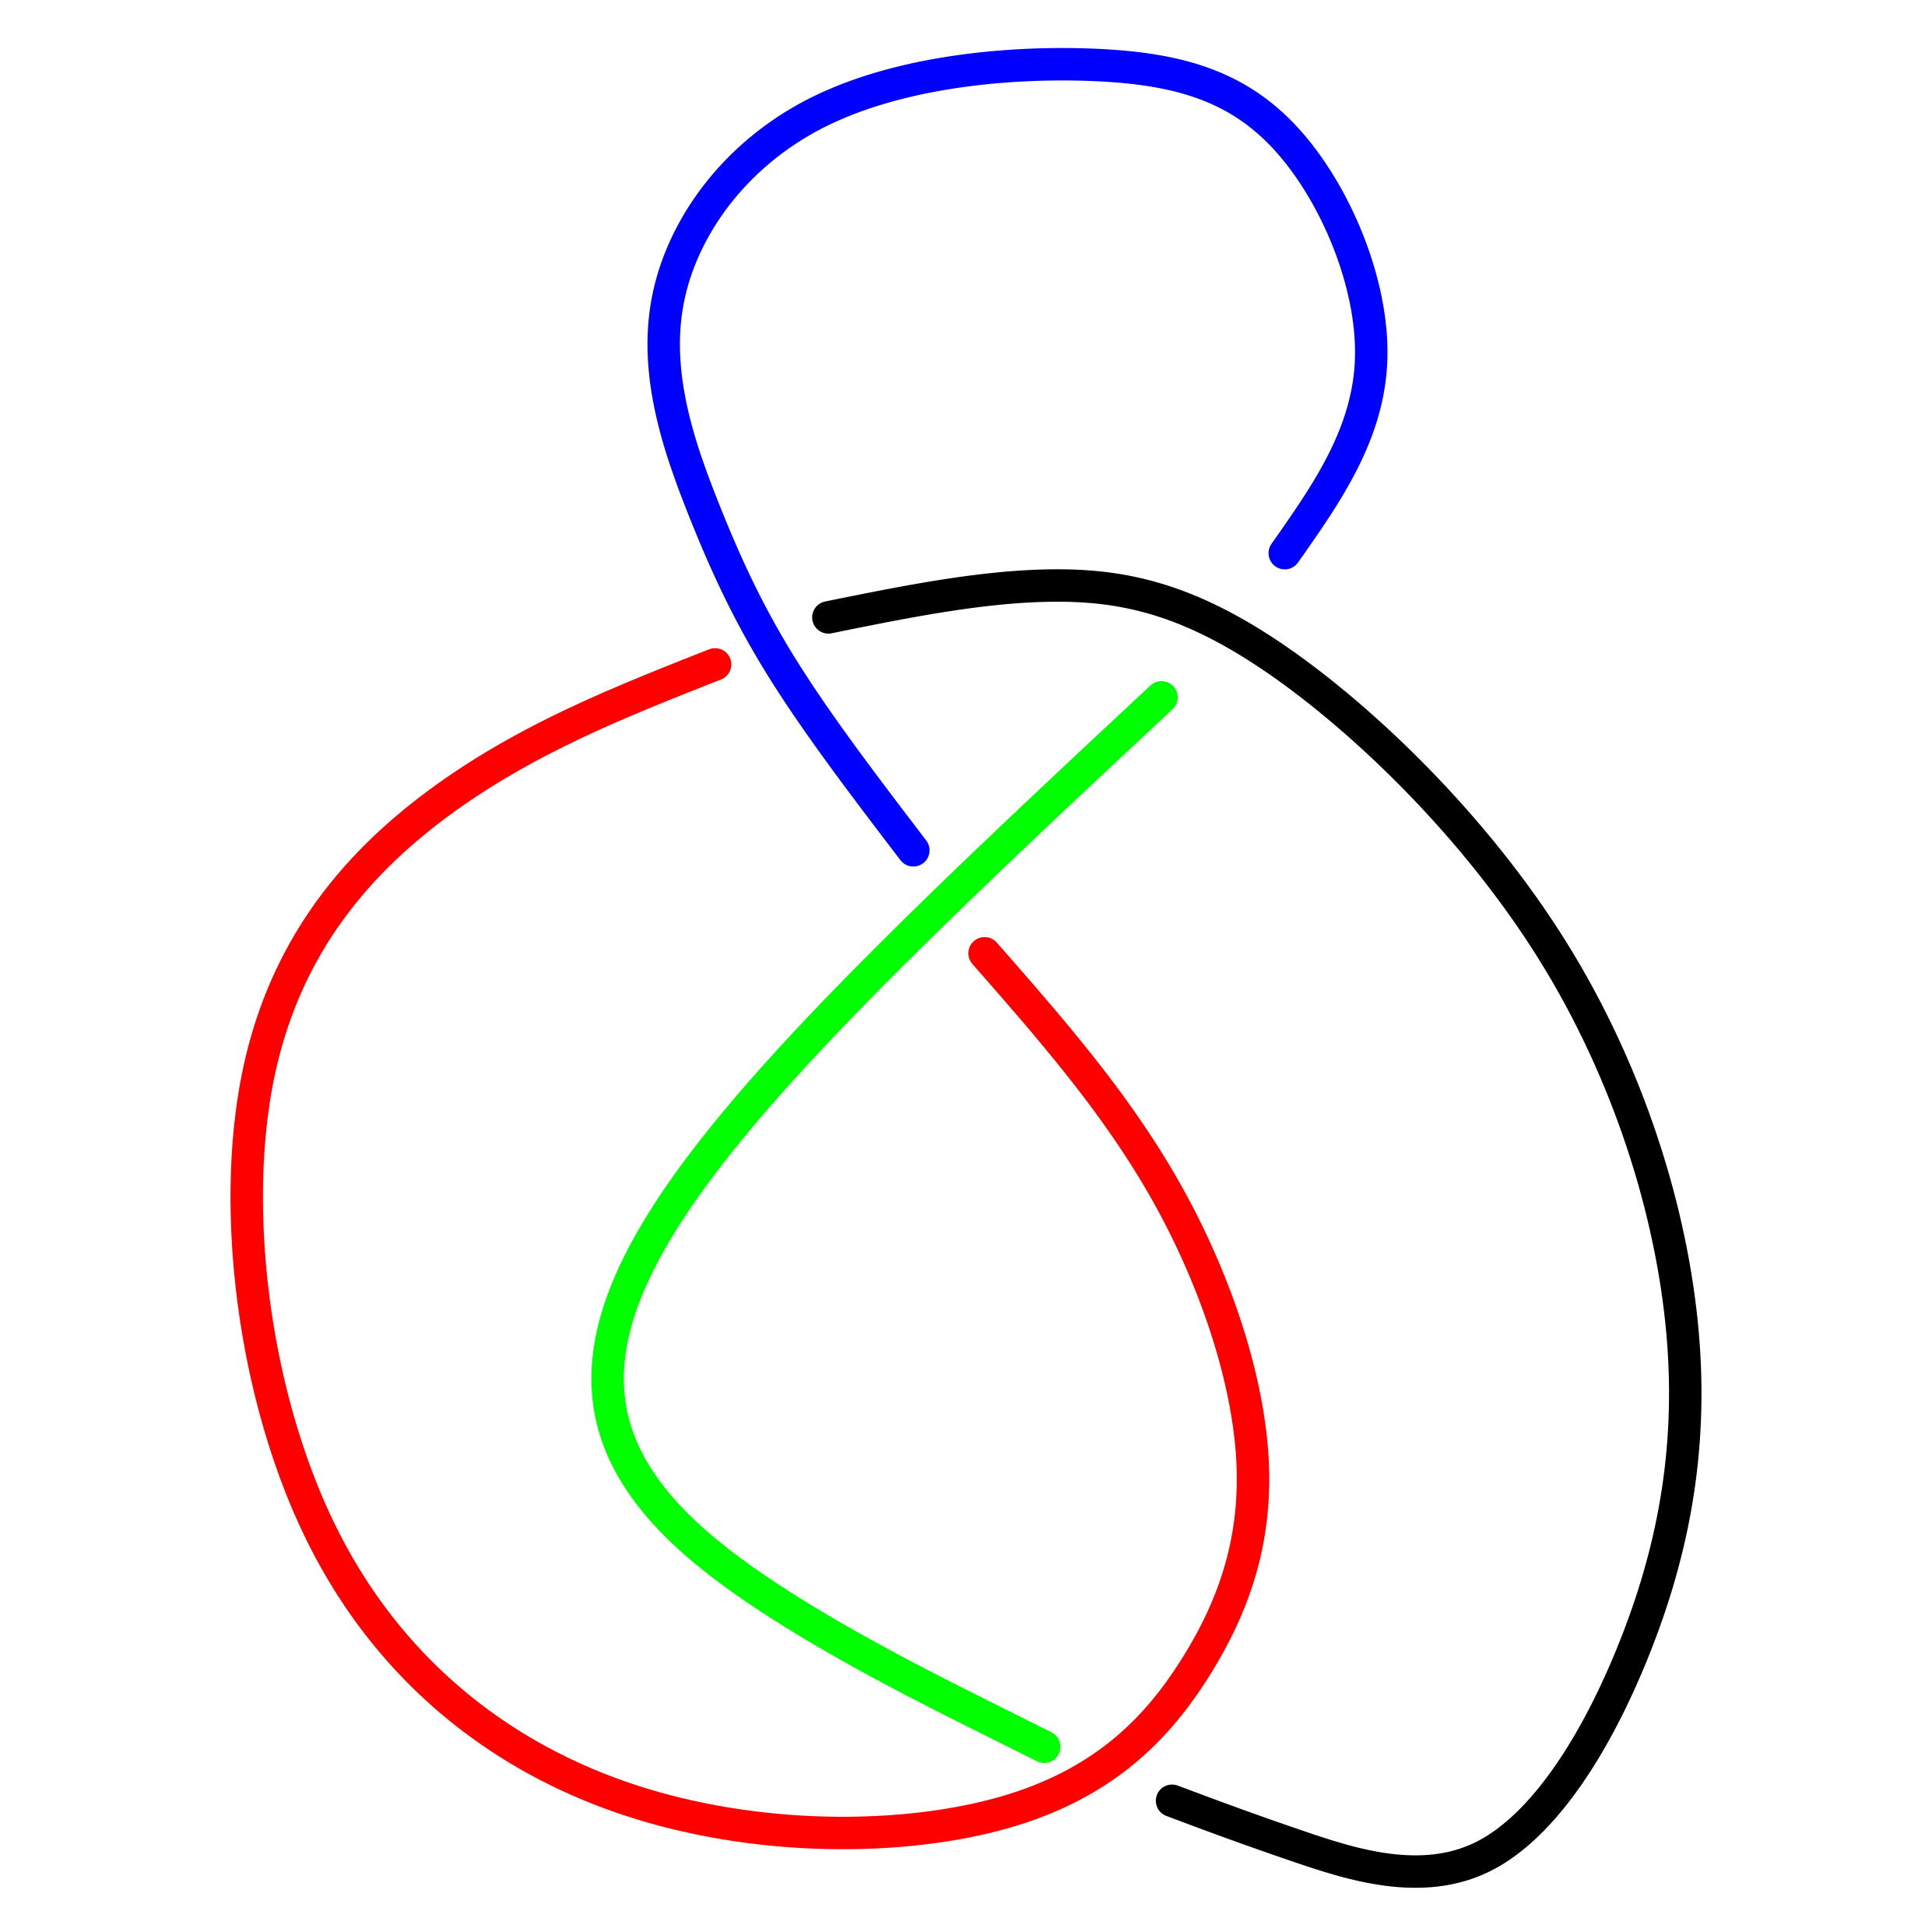
\includegraphics[width=0.5\linewidth]{picture/knotpict/knot-16}
	\caption{16th Combination}
\end{subfigure}
\qquad
\begin{subfigure}[b]{0.25\linewidth}
	\centering
	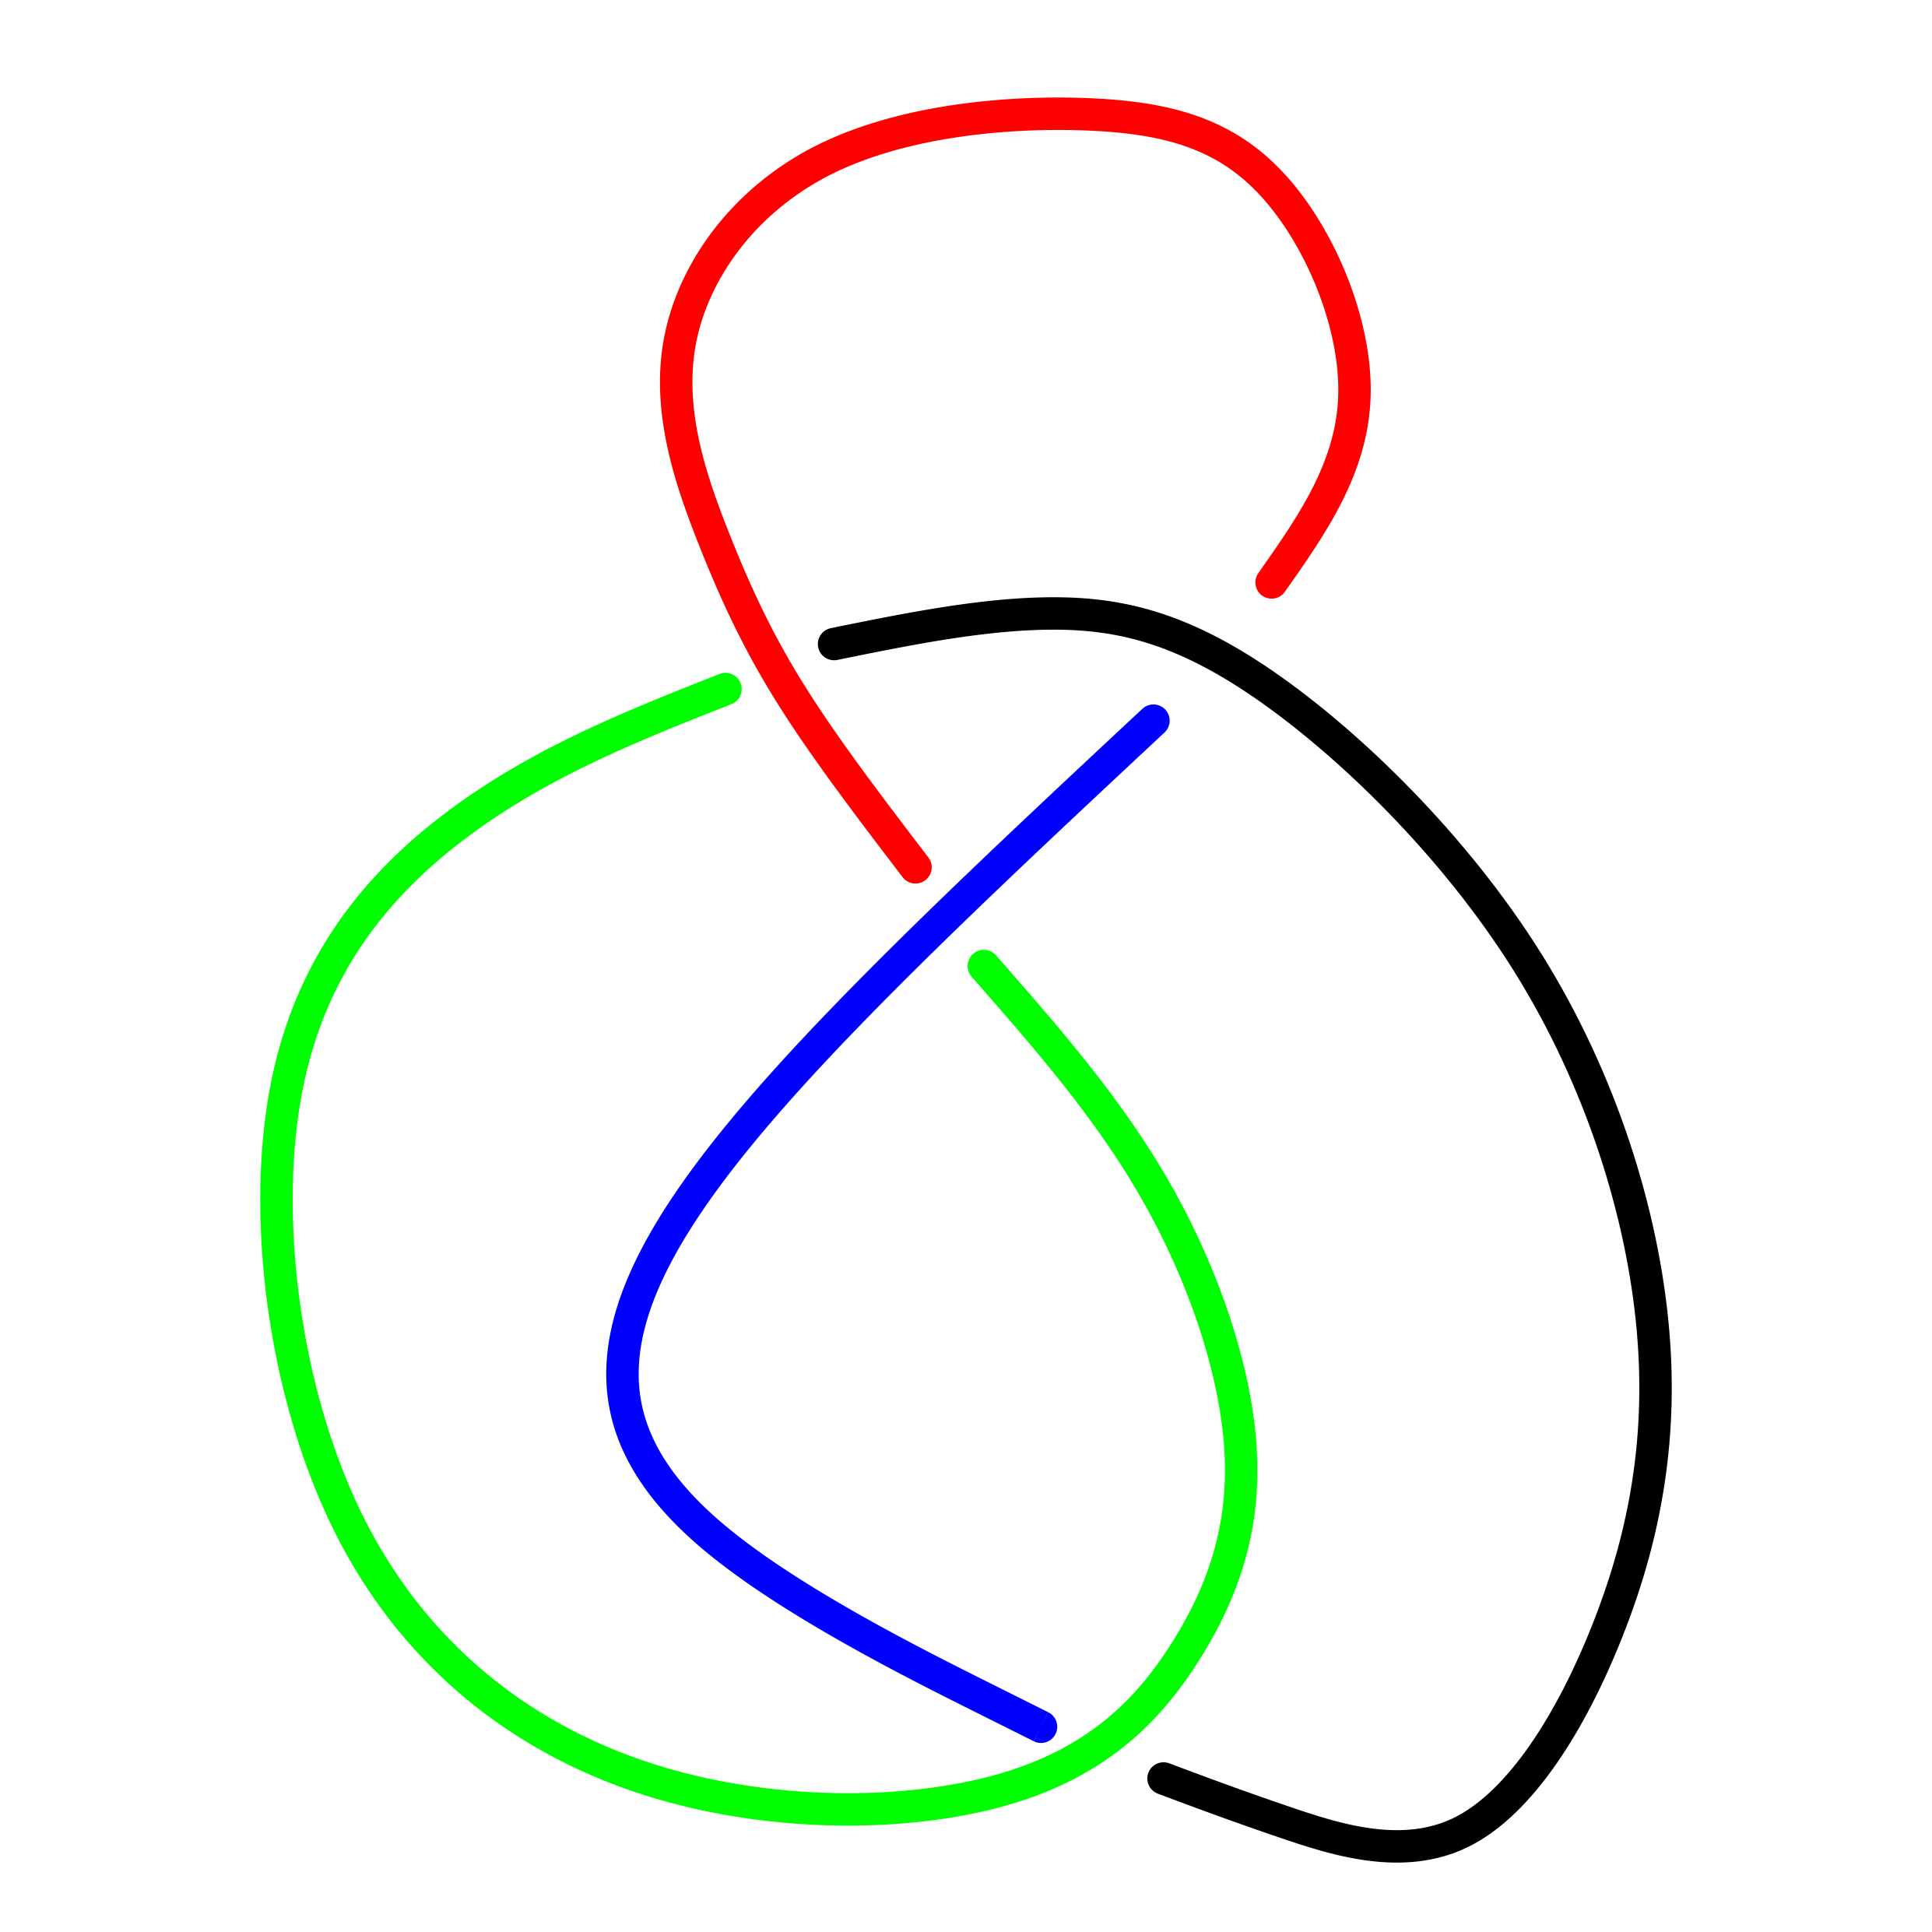
\includegraphics[width=0.5\linewidth]{picture/knotpict/knot-17}
	\caption{17th Combination}
\end{subfigure}
\qquad
\begin{subfigure}[b]{0.25\linewidth}
	\centering
	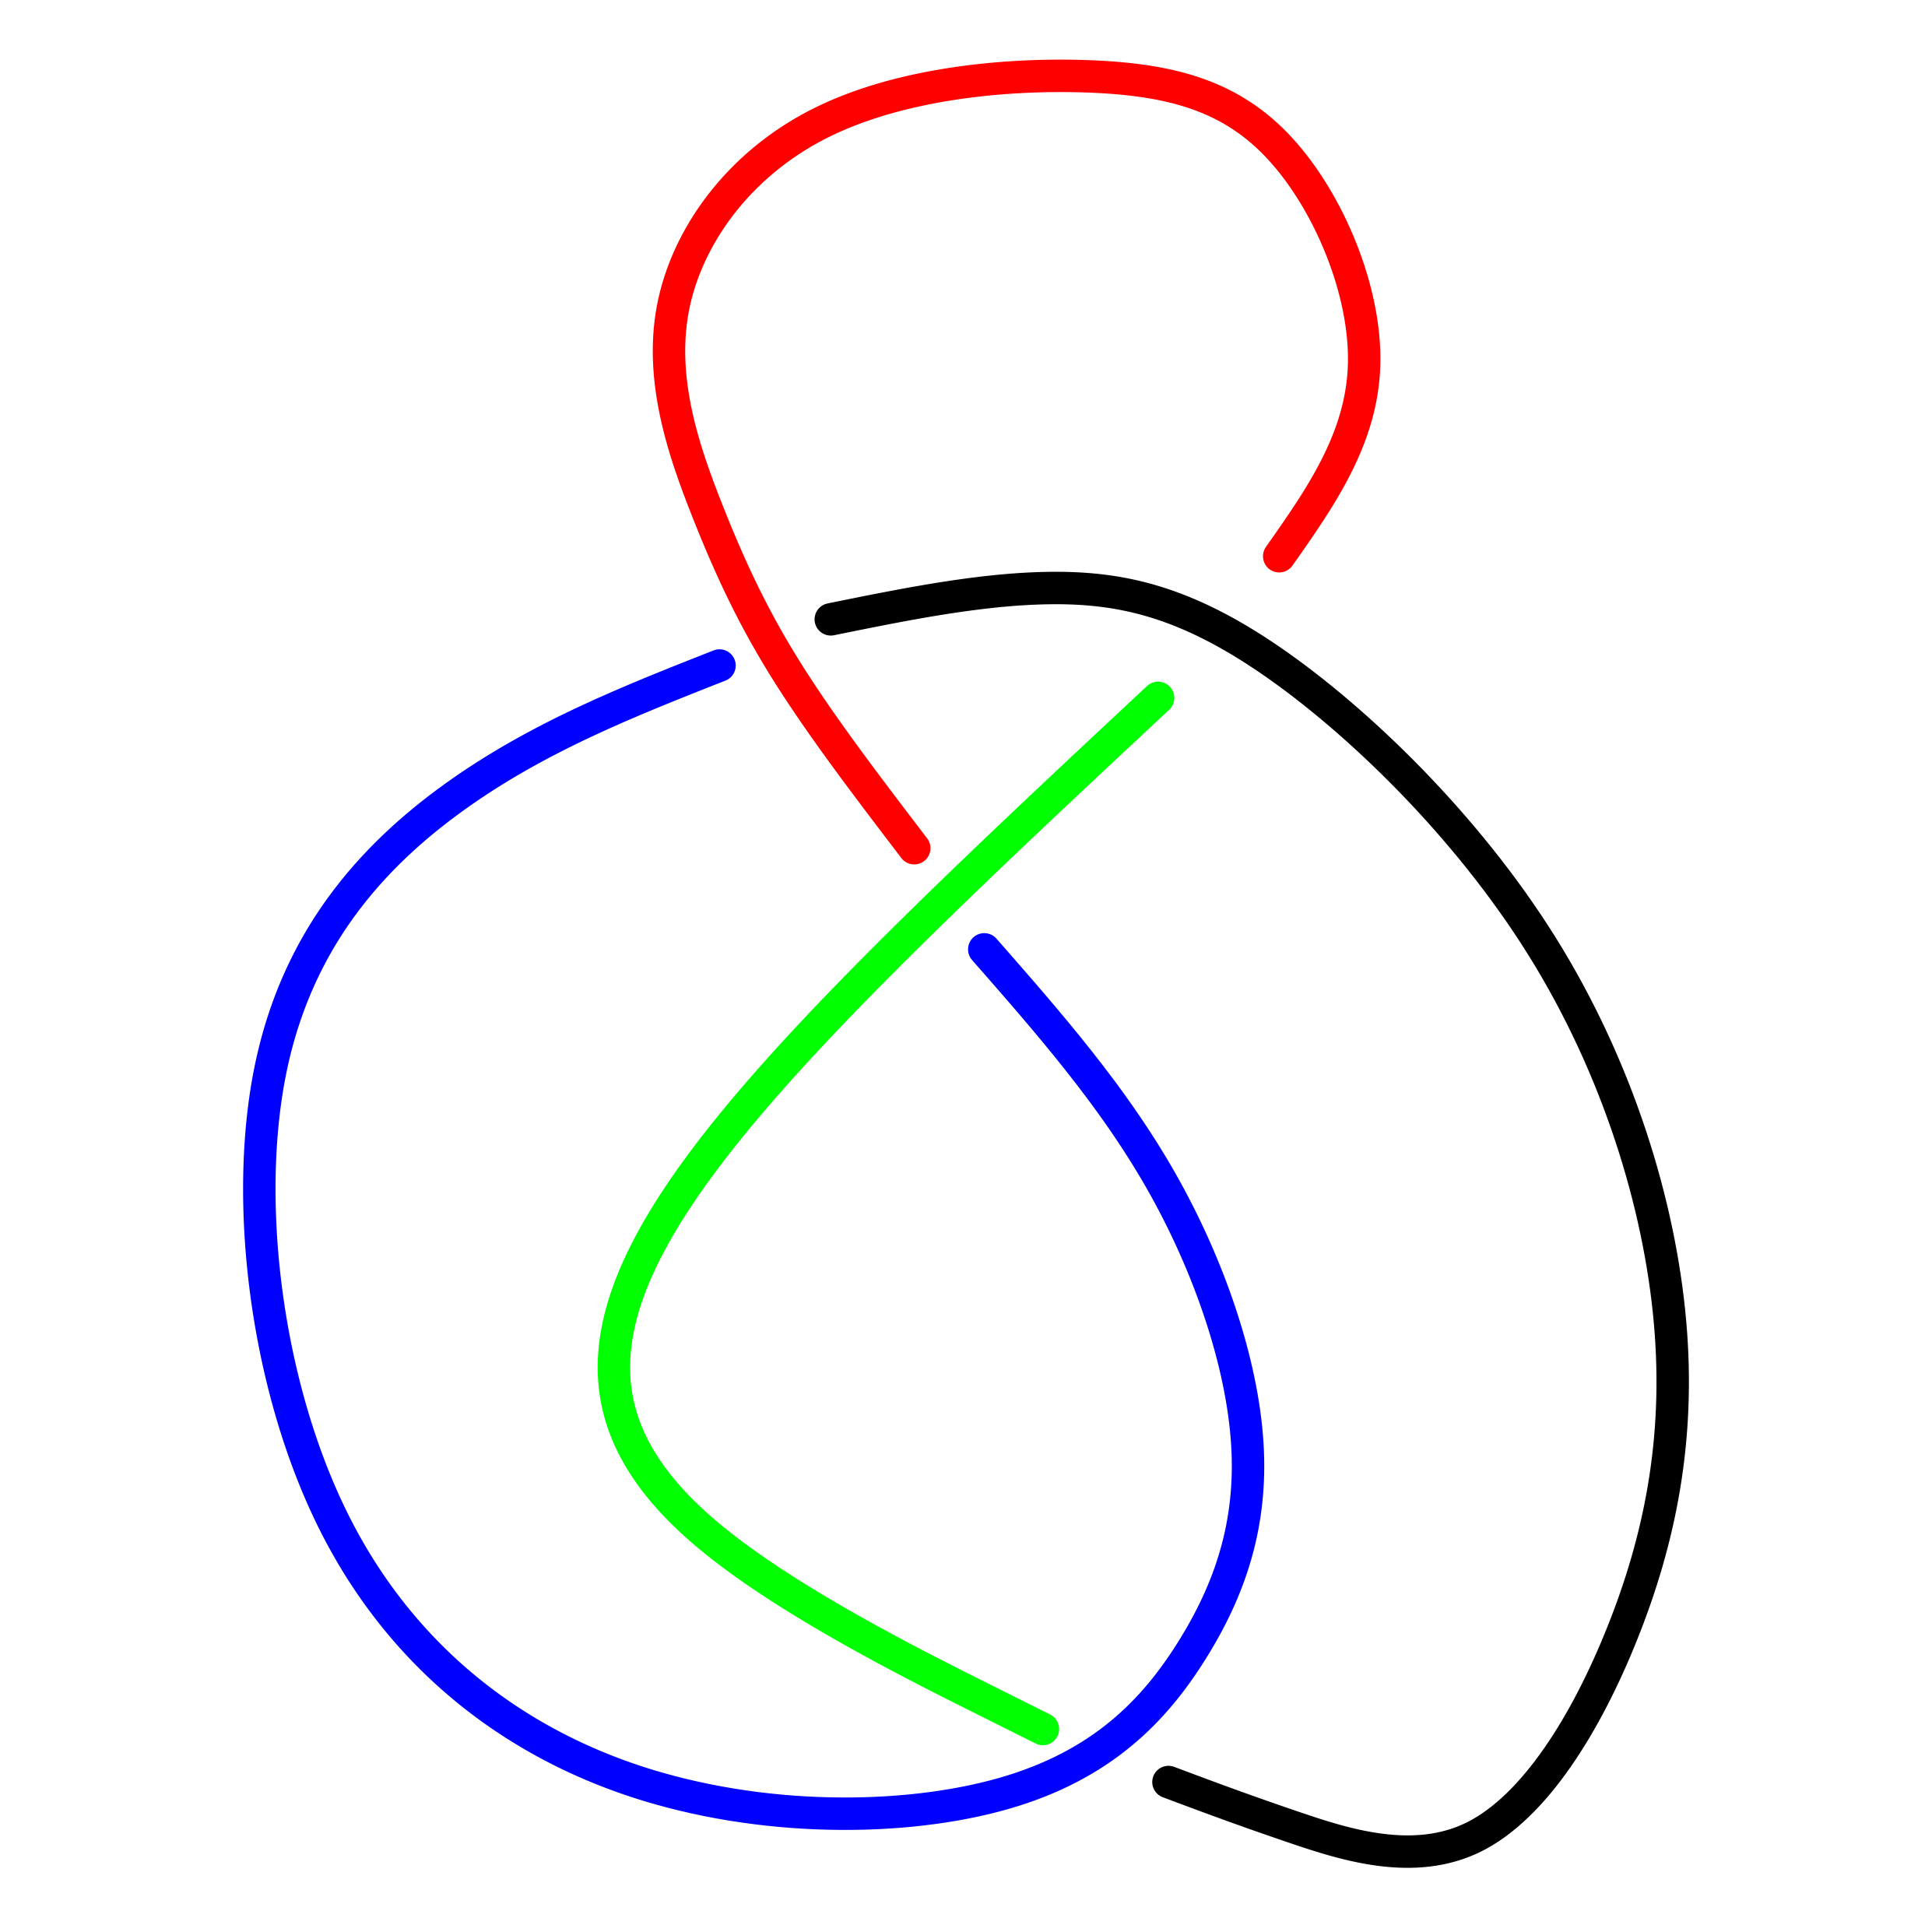
\includegraphics[width=0.5\linewidth]{picture/knotpict/knot-18}
	\caption{18th Combination}
\end{subfigure}
\qquad
\begin{subfigure}[b]{0.25\linewidth}
	\centering
	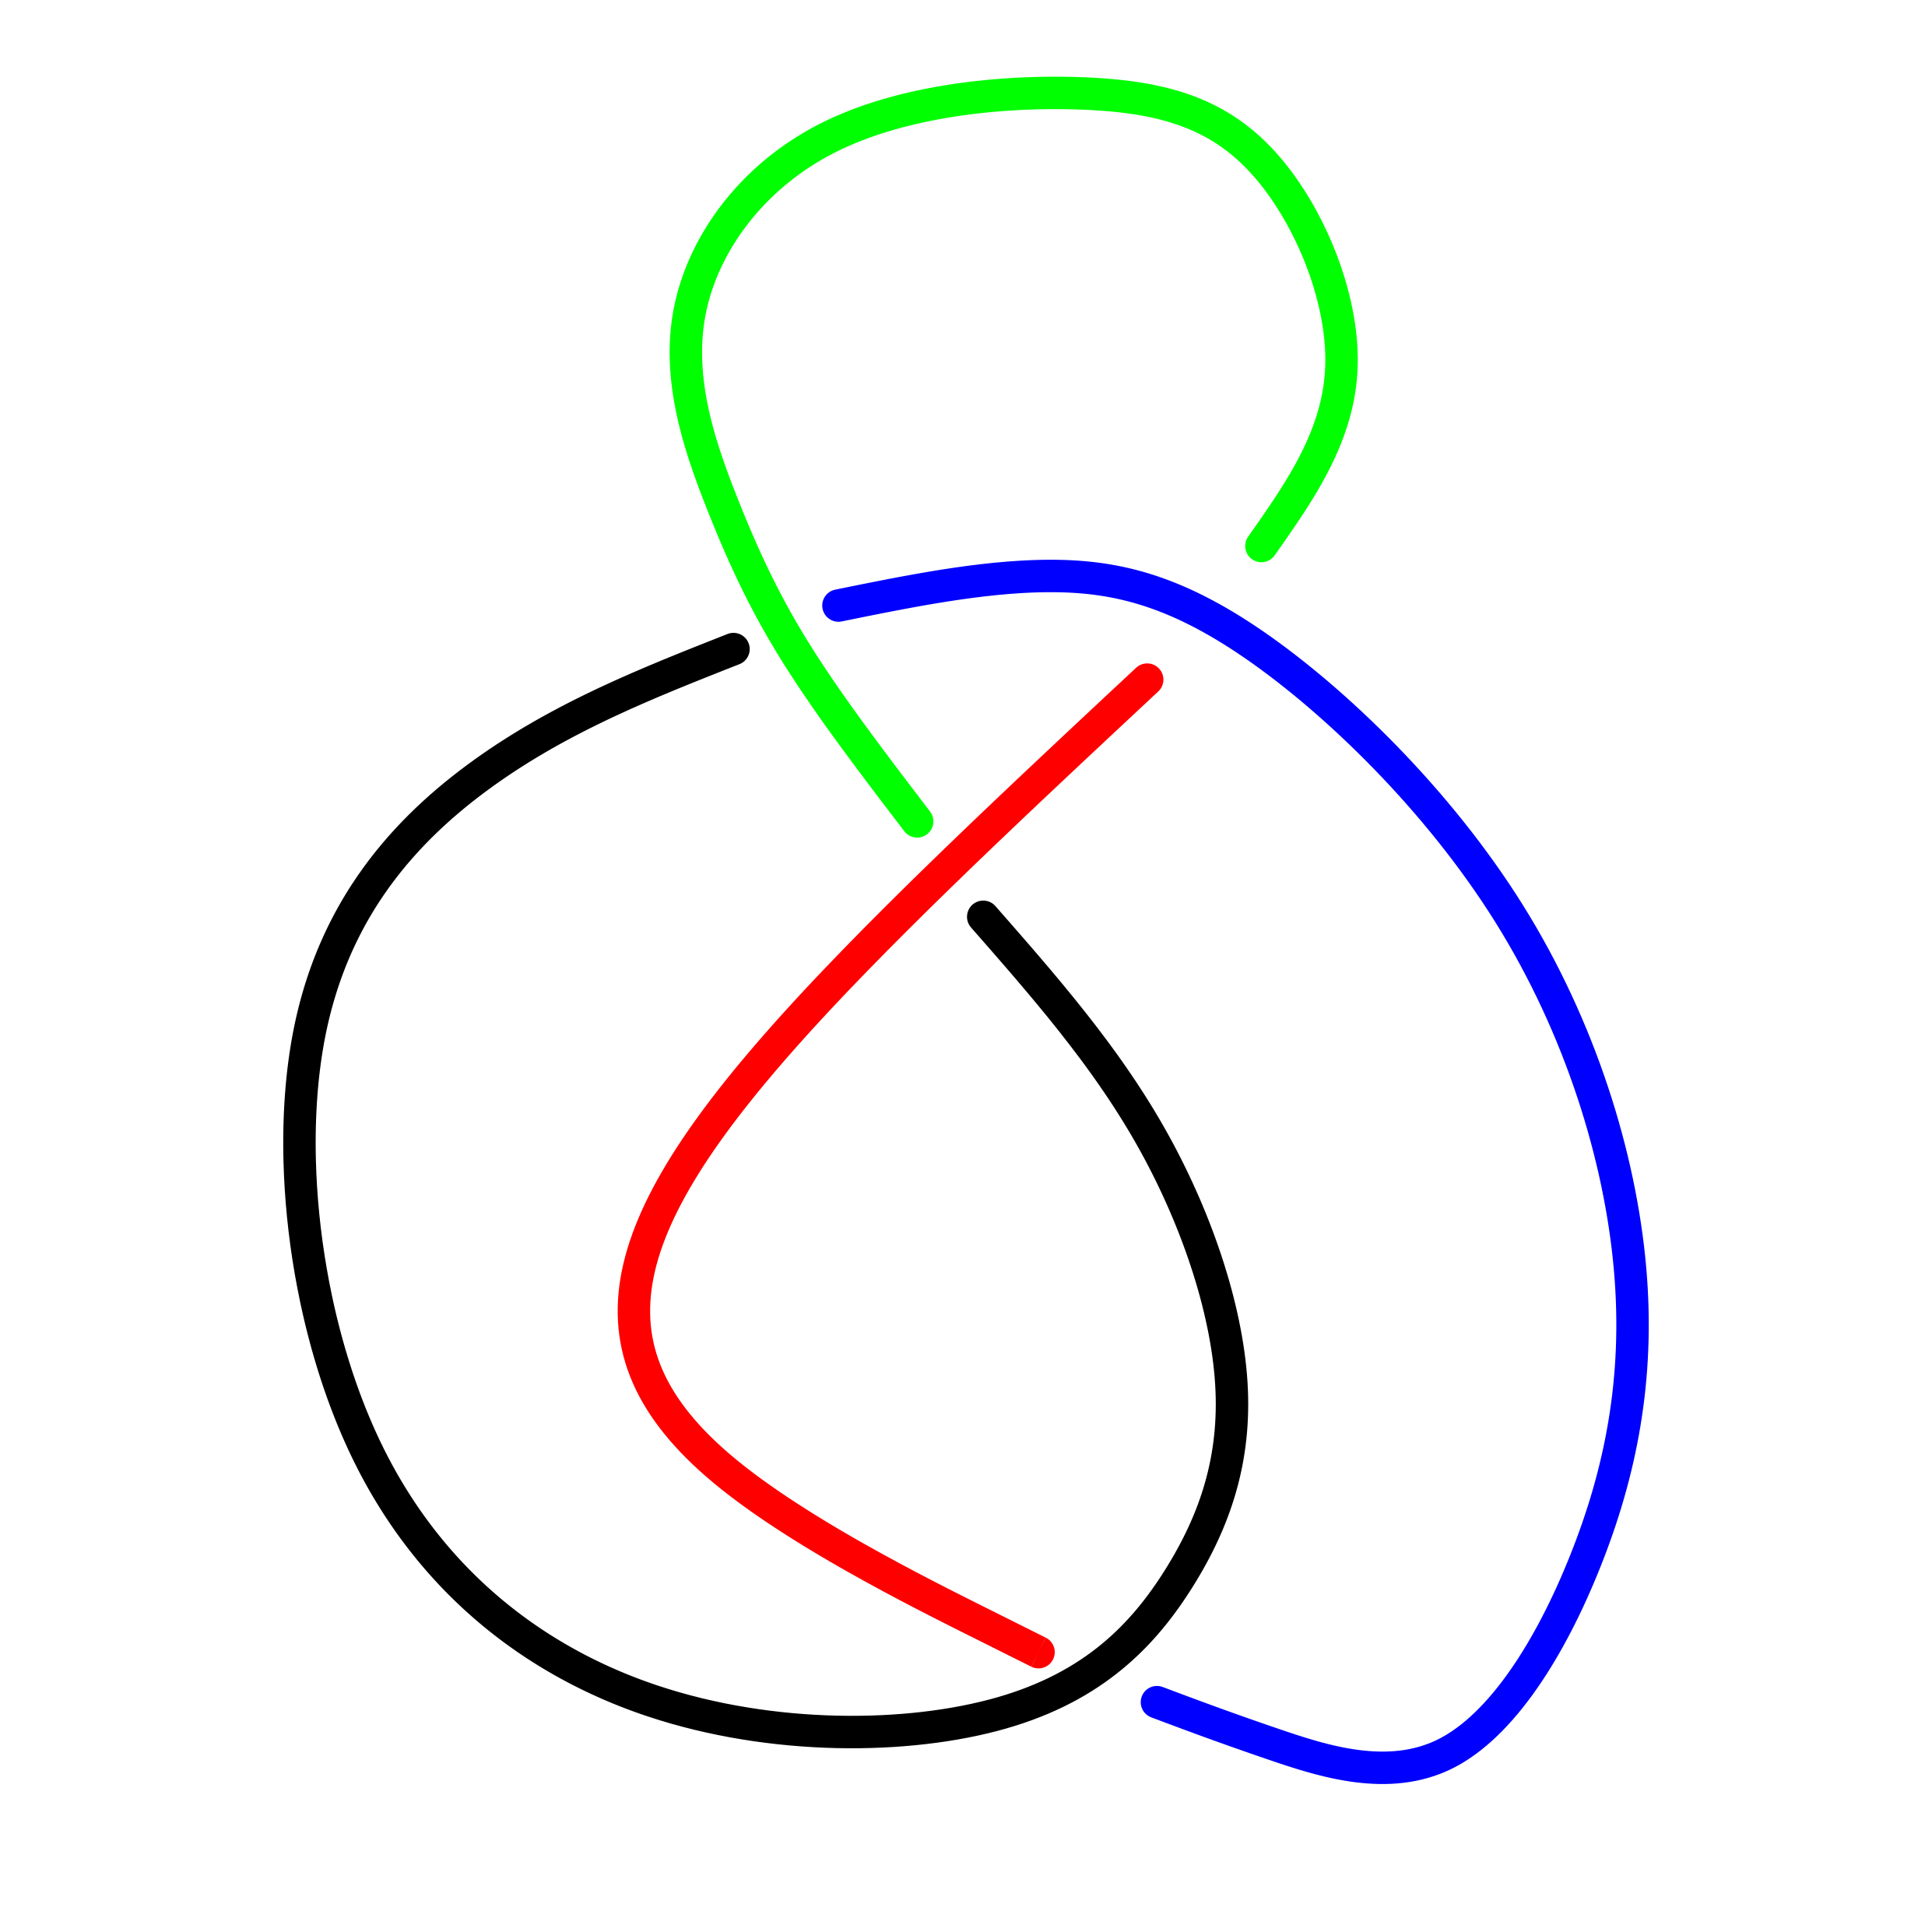
\includegraphics[width=0.5\linewidth]{picture/knotpict/knot-19}
	\caption{19th Combination}
\end{subfigure}
\qquad
\begin{subfigure}[b]{0.25\linewidth}
	\centering
	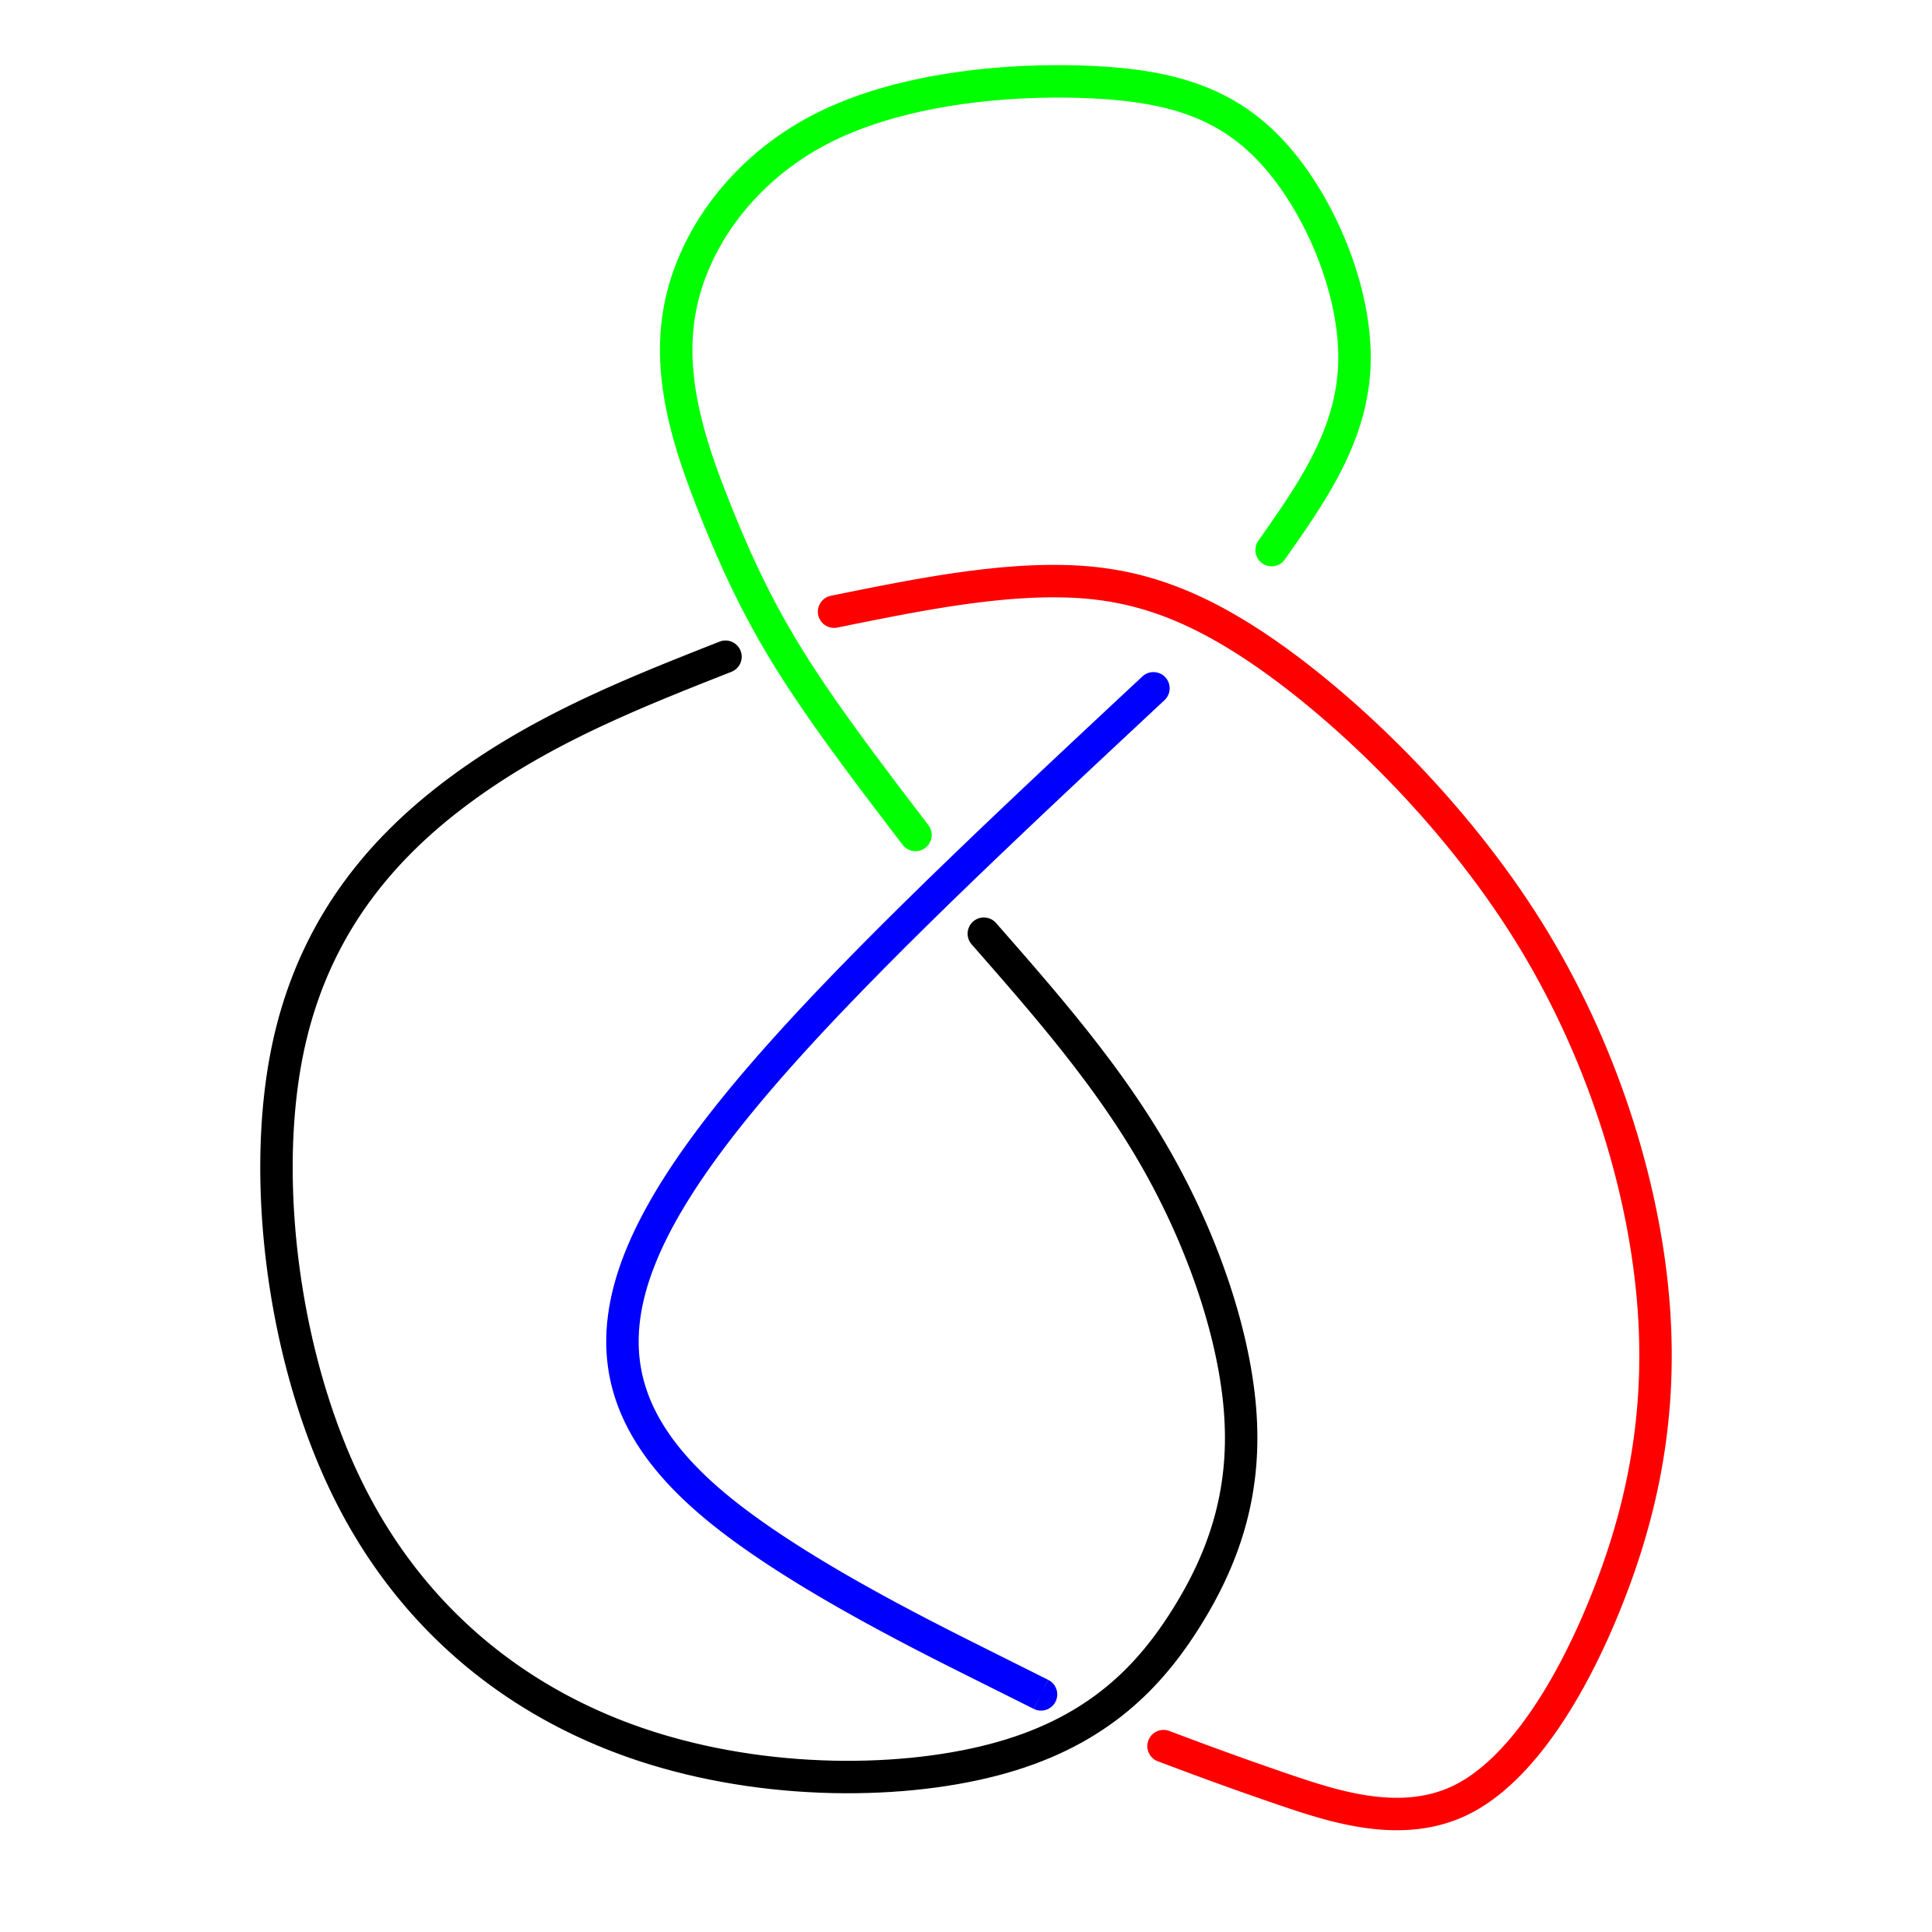
\includegraphics[width=0.5\linewidth]{picture/knotpict/knot-20}
	\caption{20th Combination}
\end{subfigure}
\qquad
\begin{subfigure}[b]{0.25\linewidth}
	\centering
	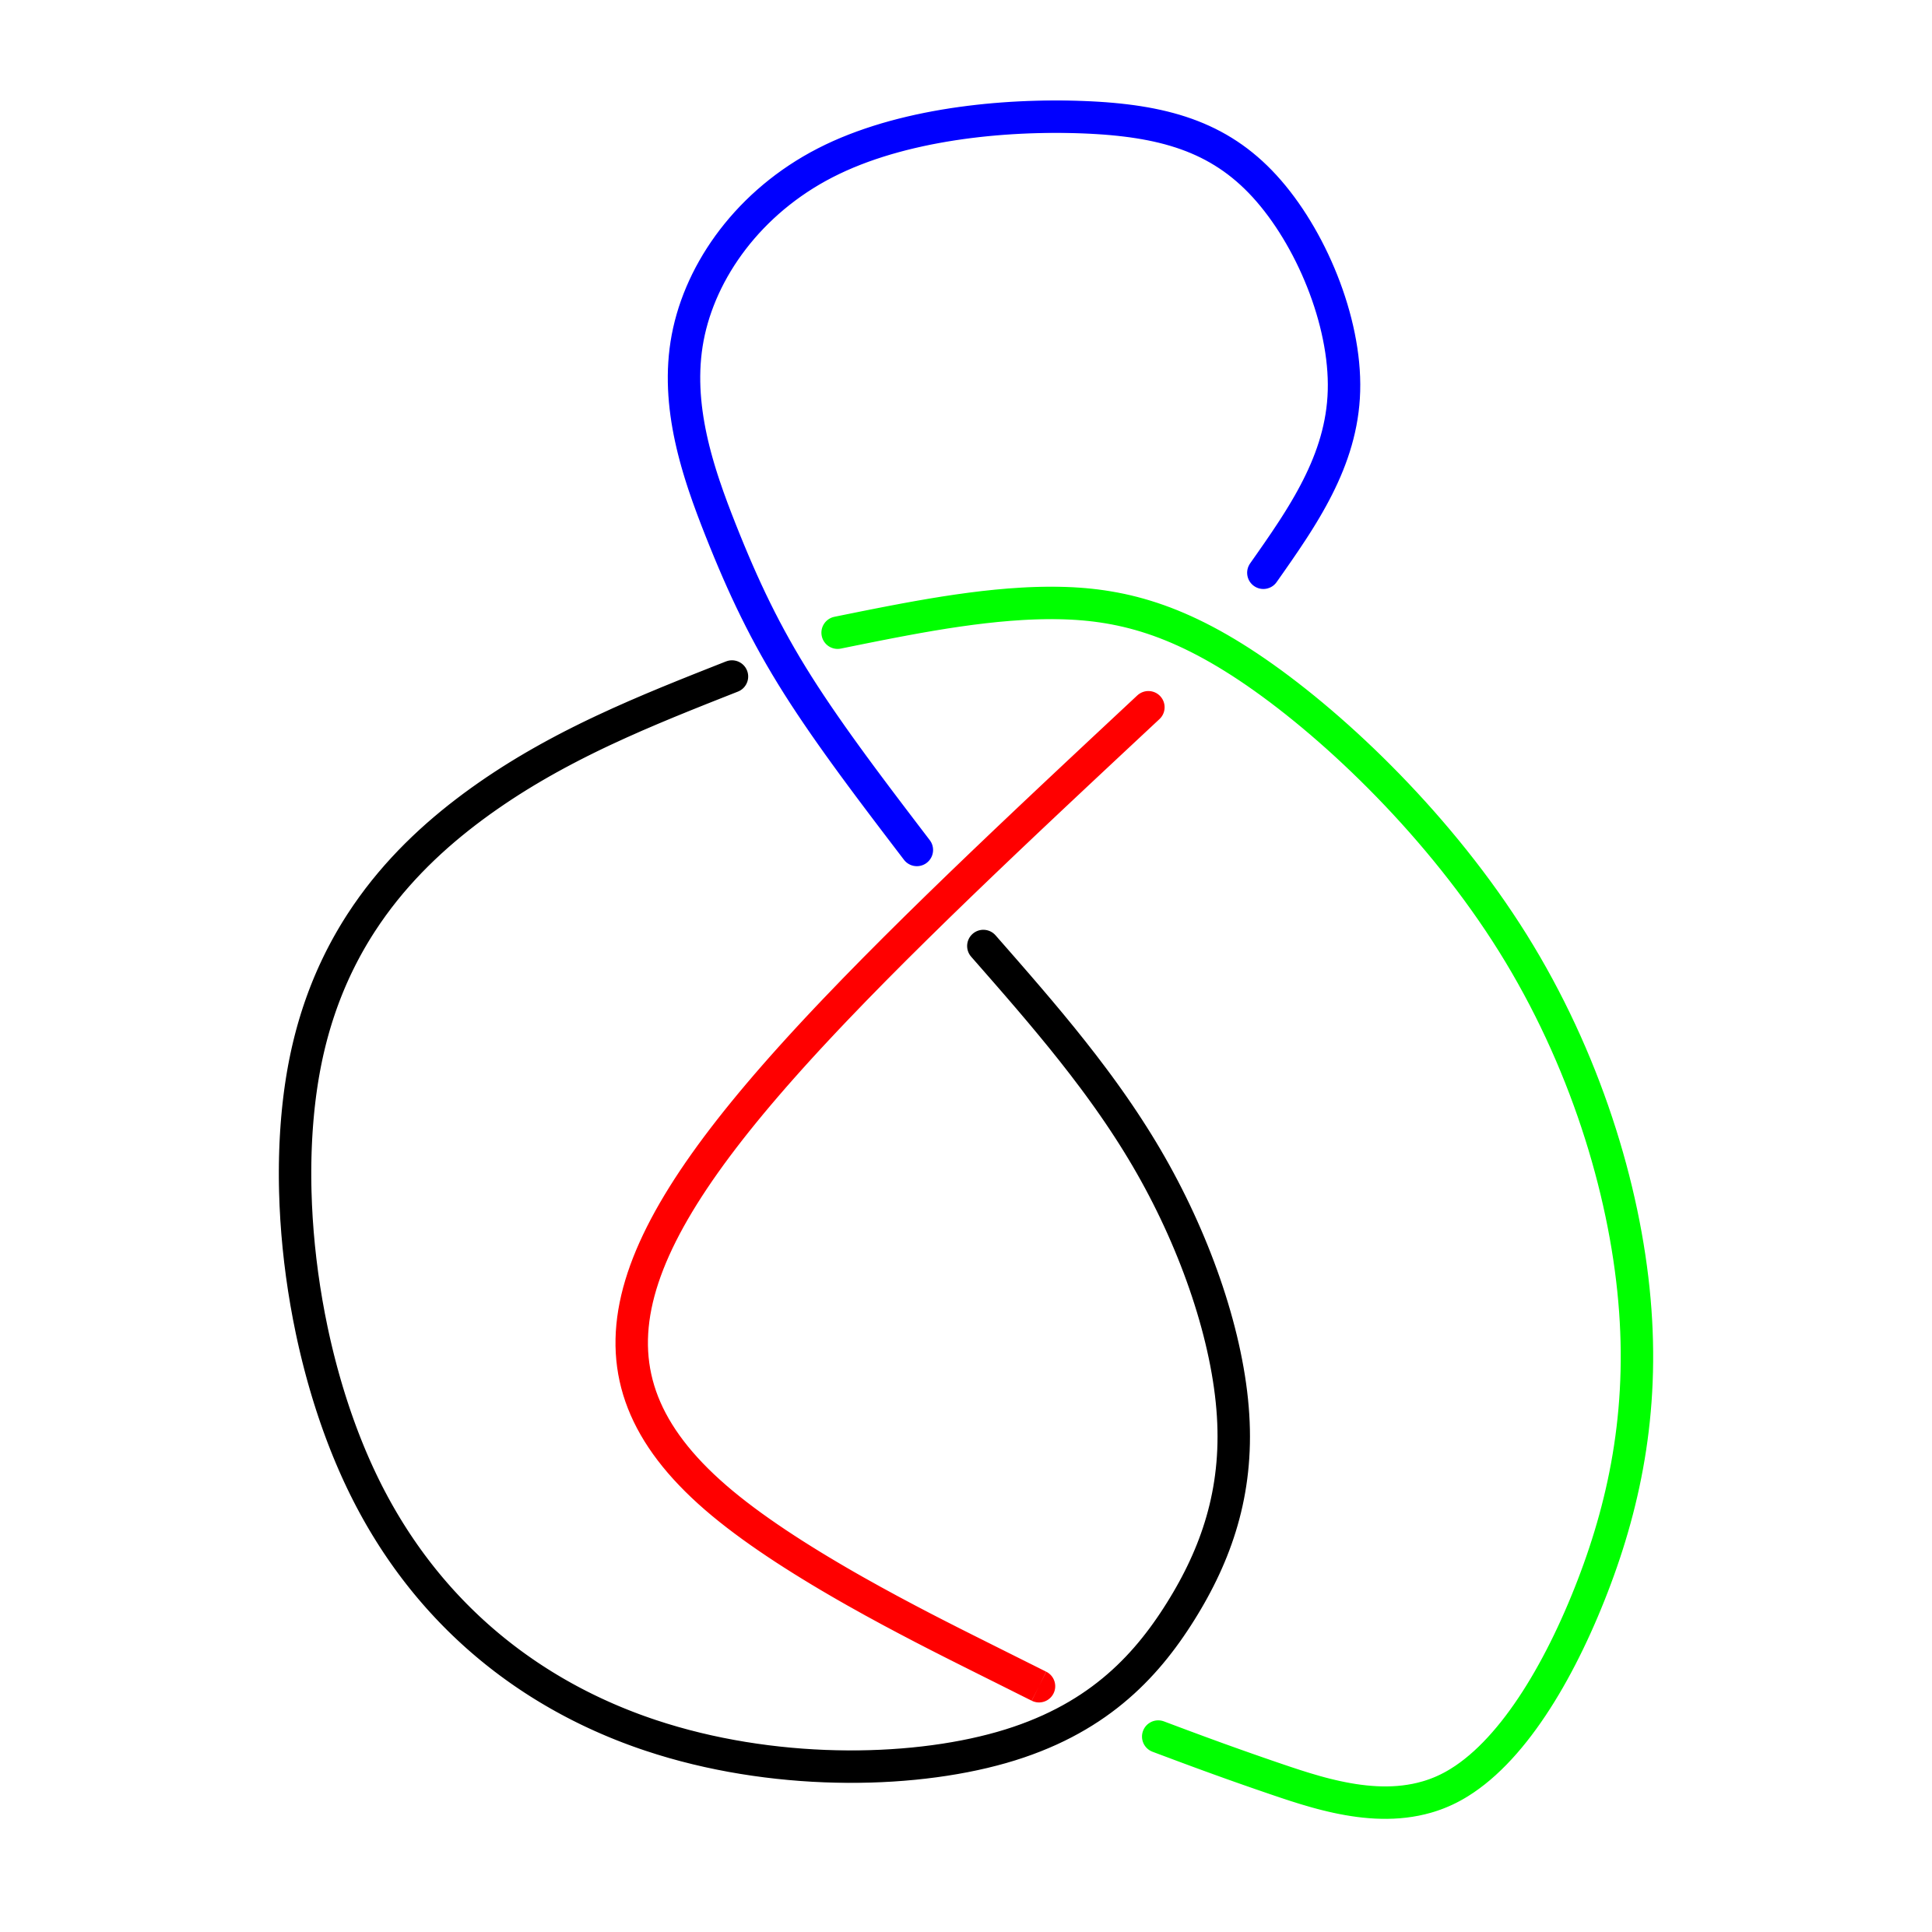
\includegraphics[width=0.5\linewidth]{picture/knotpict/knot-21}
	\caption{21th Combination}
\end{subfigure}
\qquad
\begin{subfigure}[b]{0.25\linewidth}
	\centering
	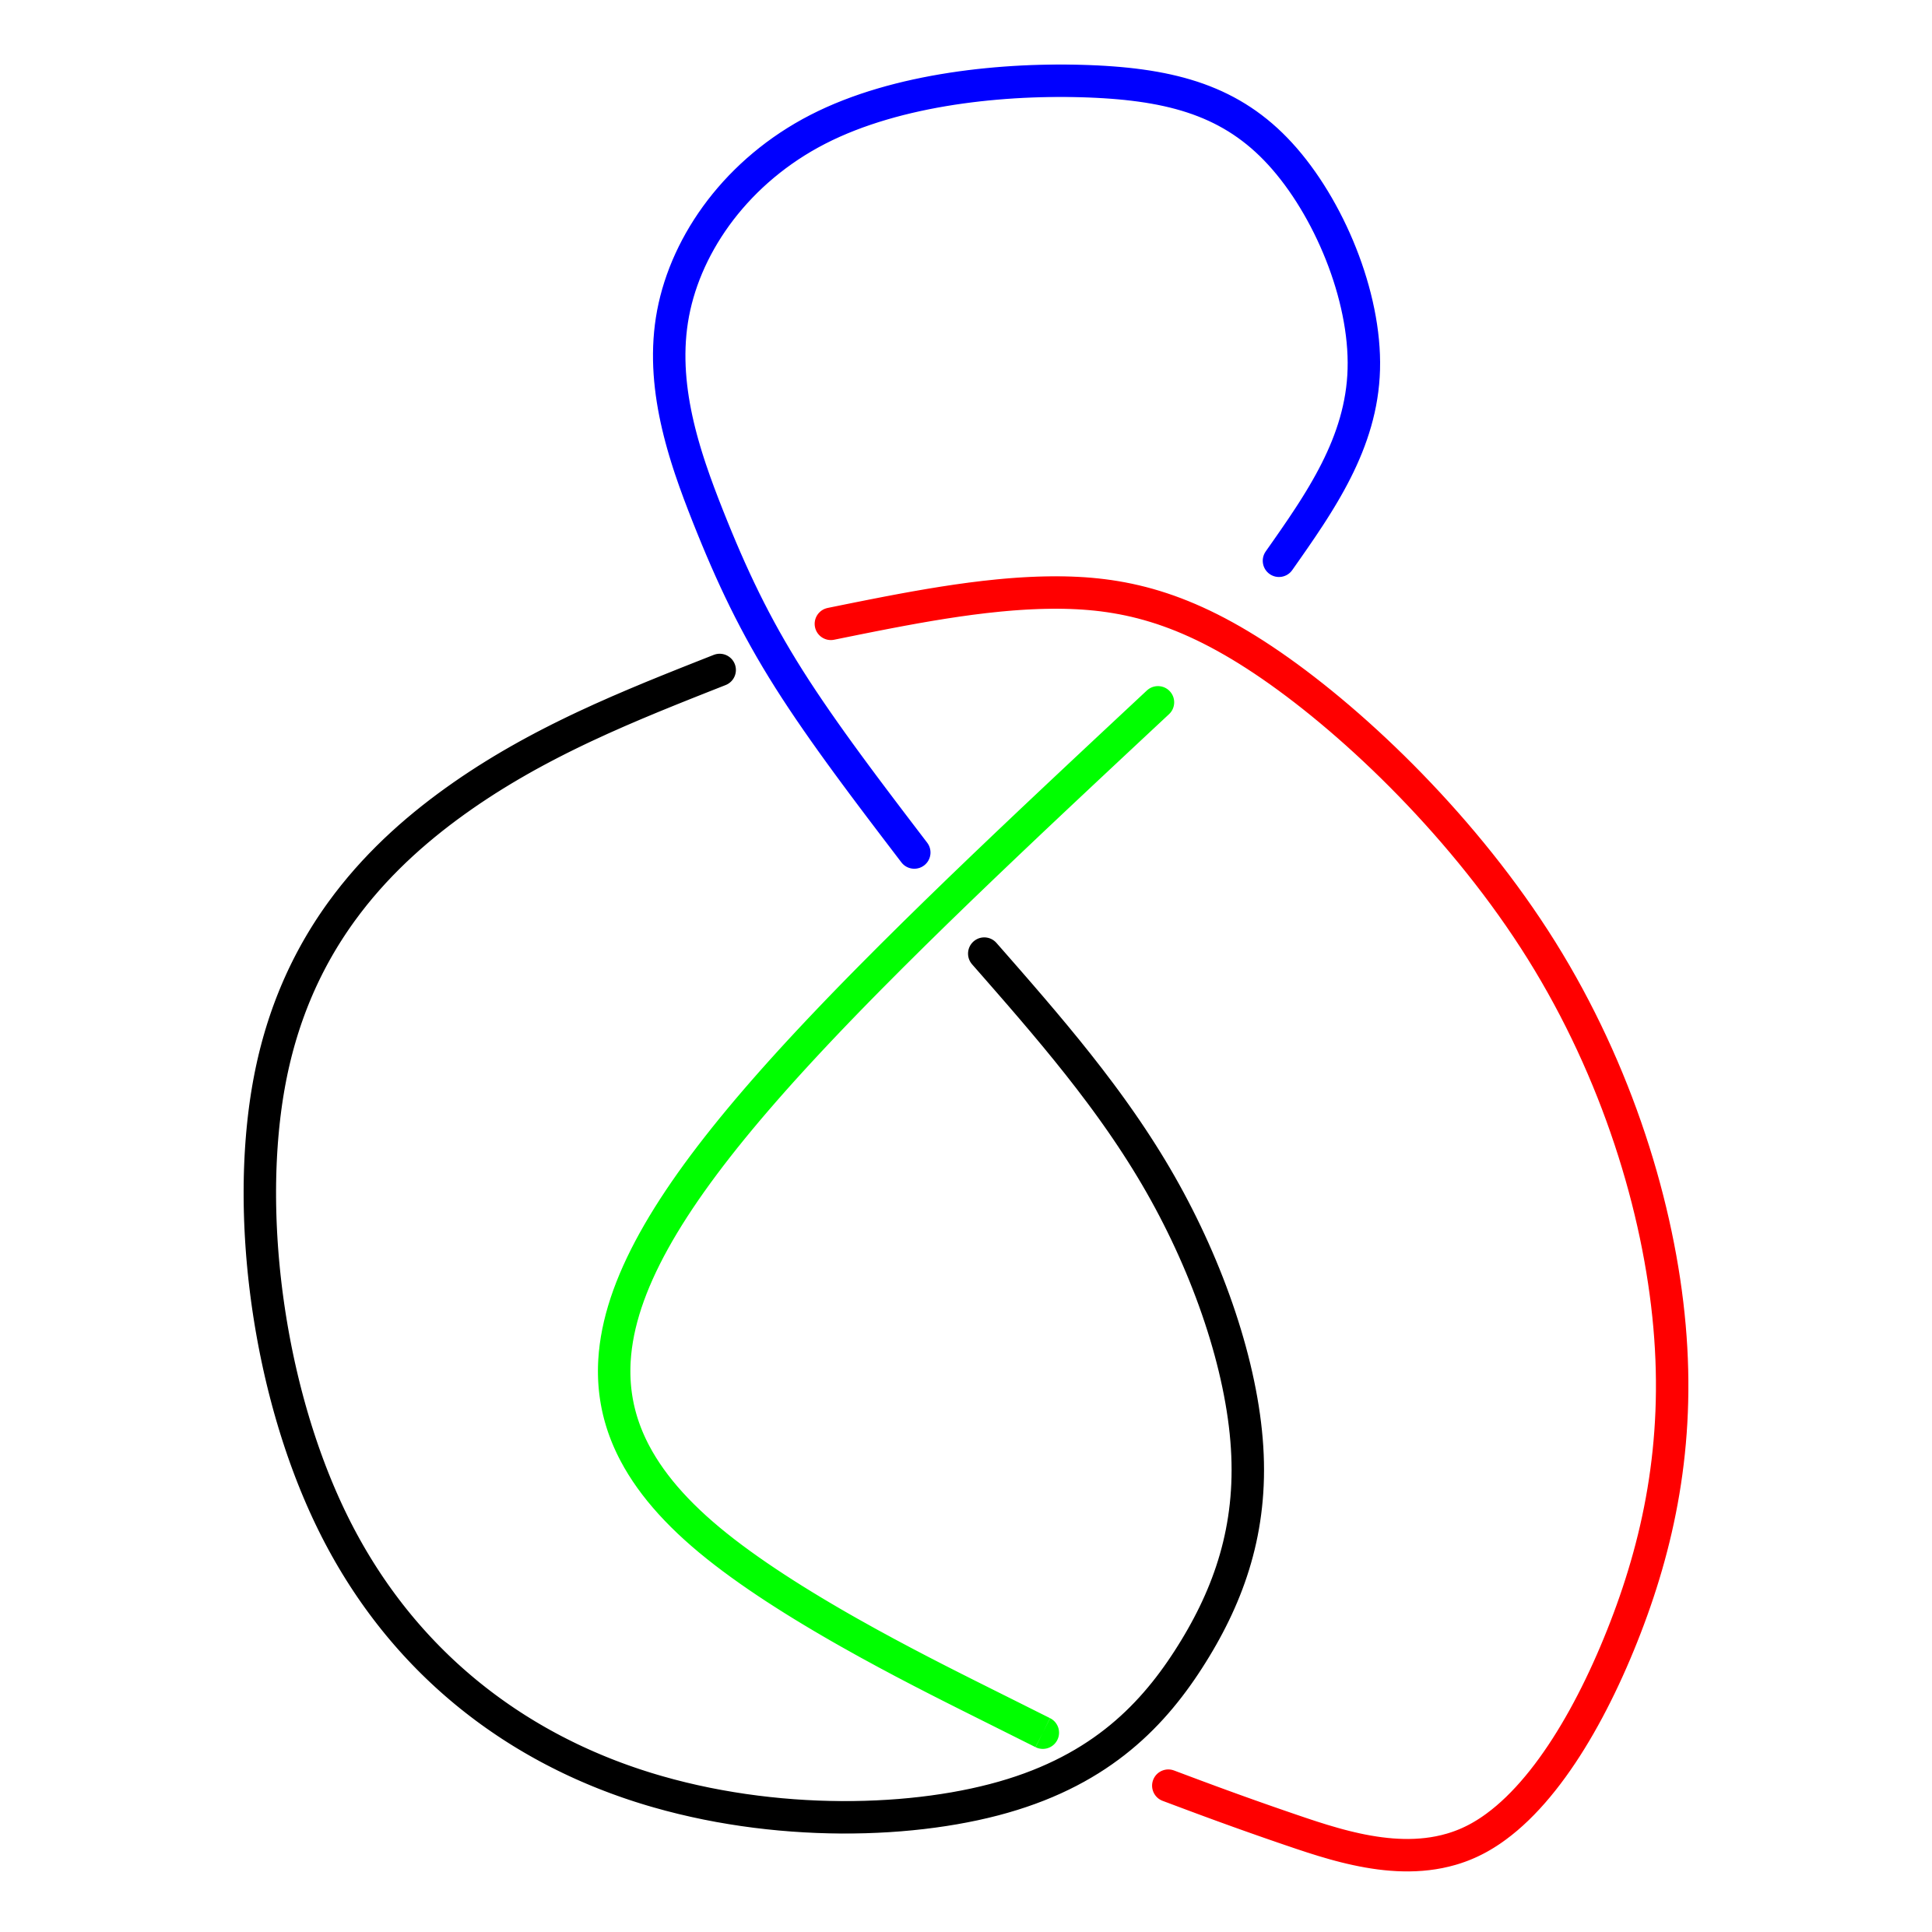
\includegraphics[width=0.5\linewidth]{picture/knotpict/knot-22}
	\caption{22nd Combination}
\end{subfigure}
\qquad
\begin{subfigure}[b]{0.25\linewidth}
	\centering
	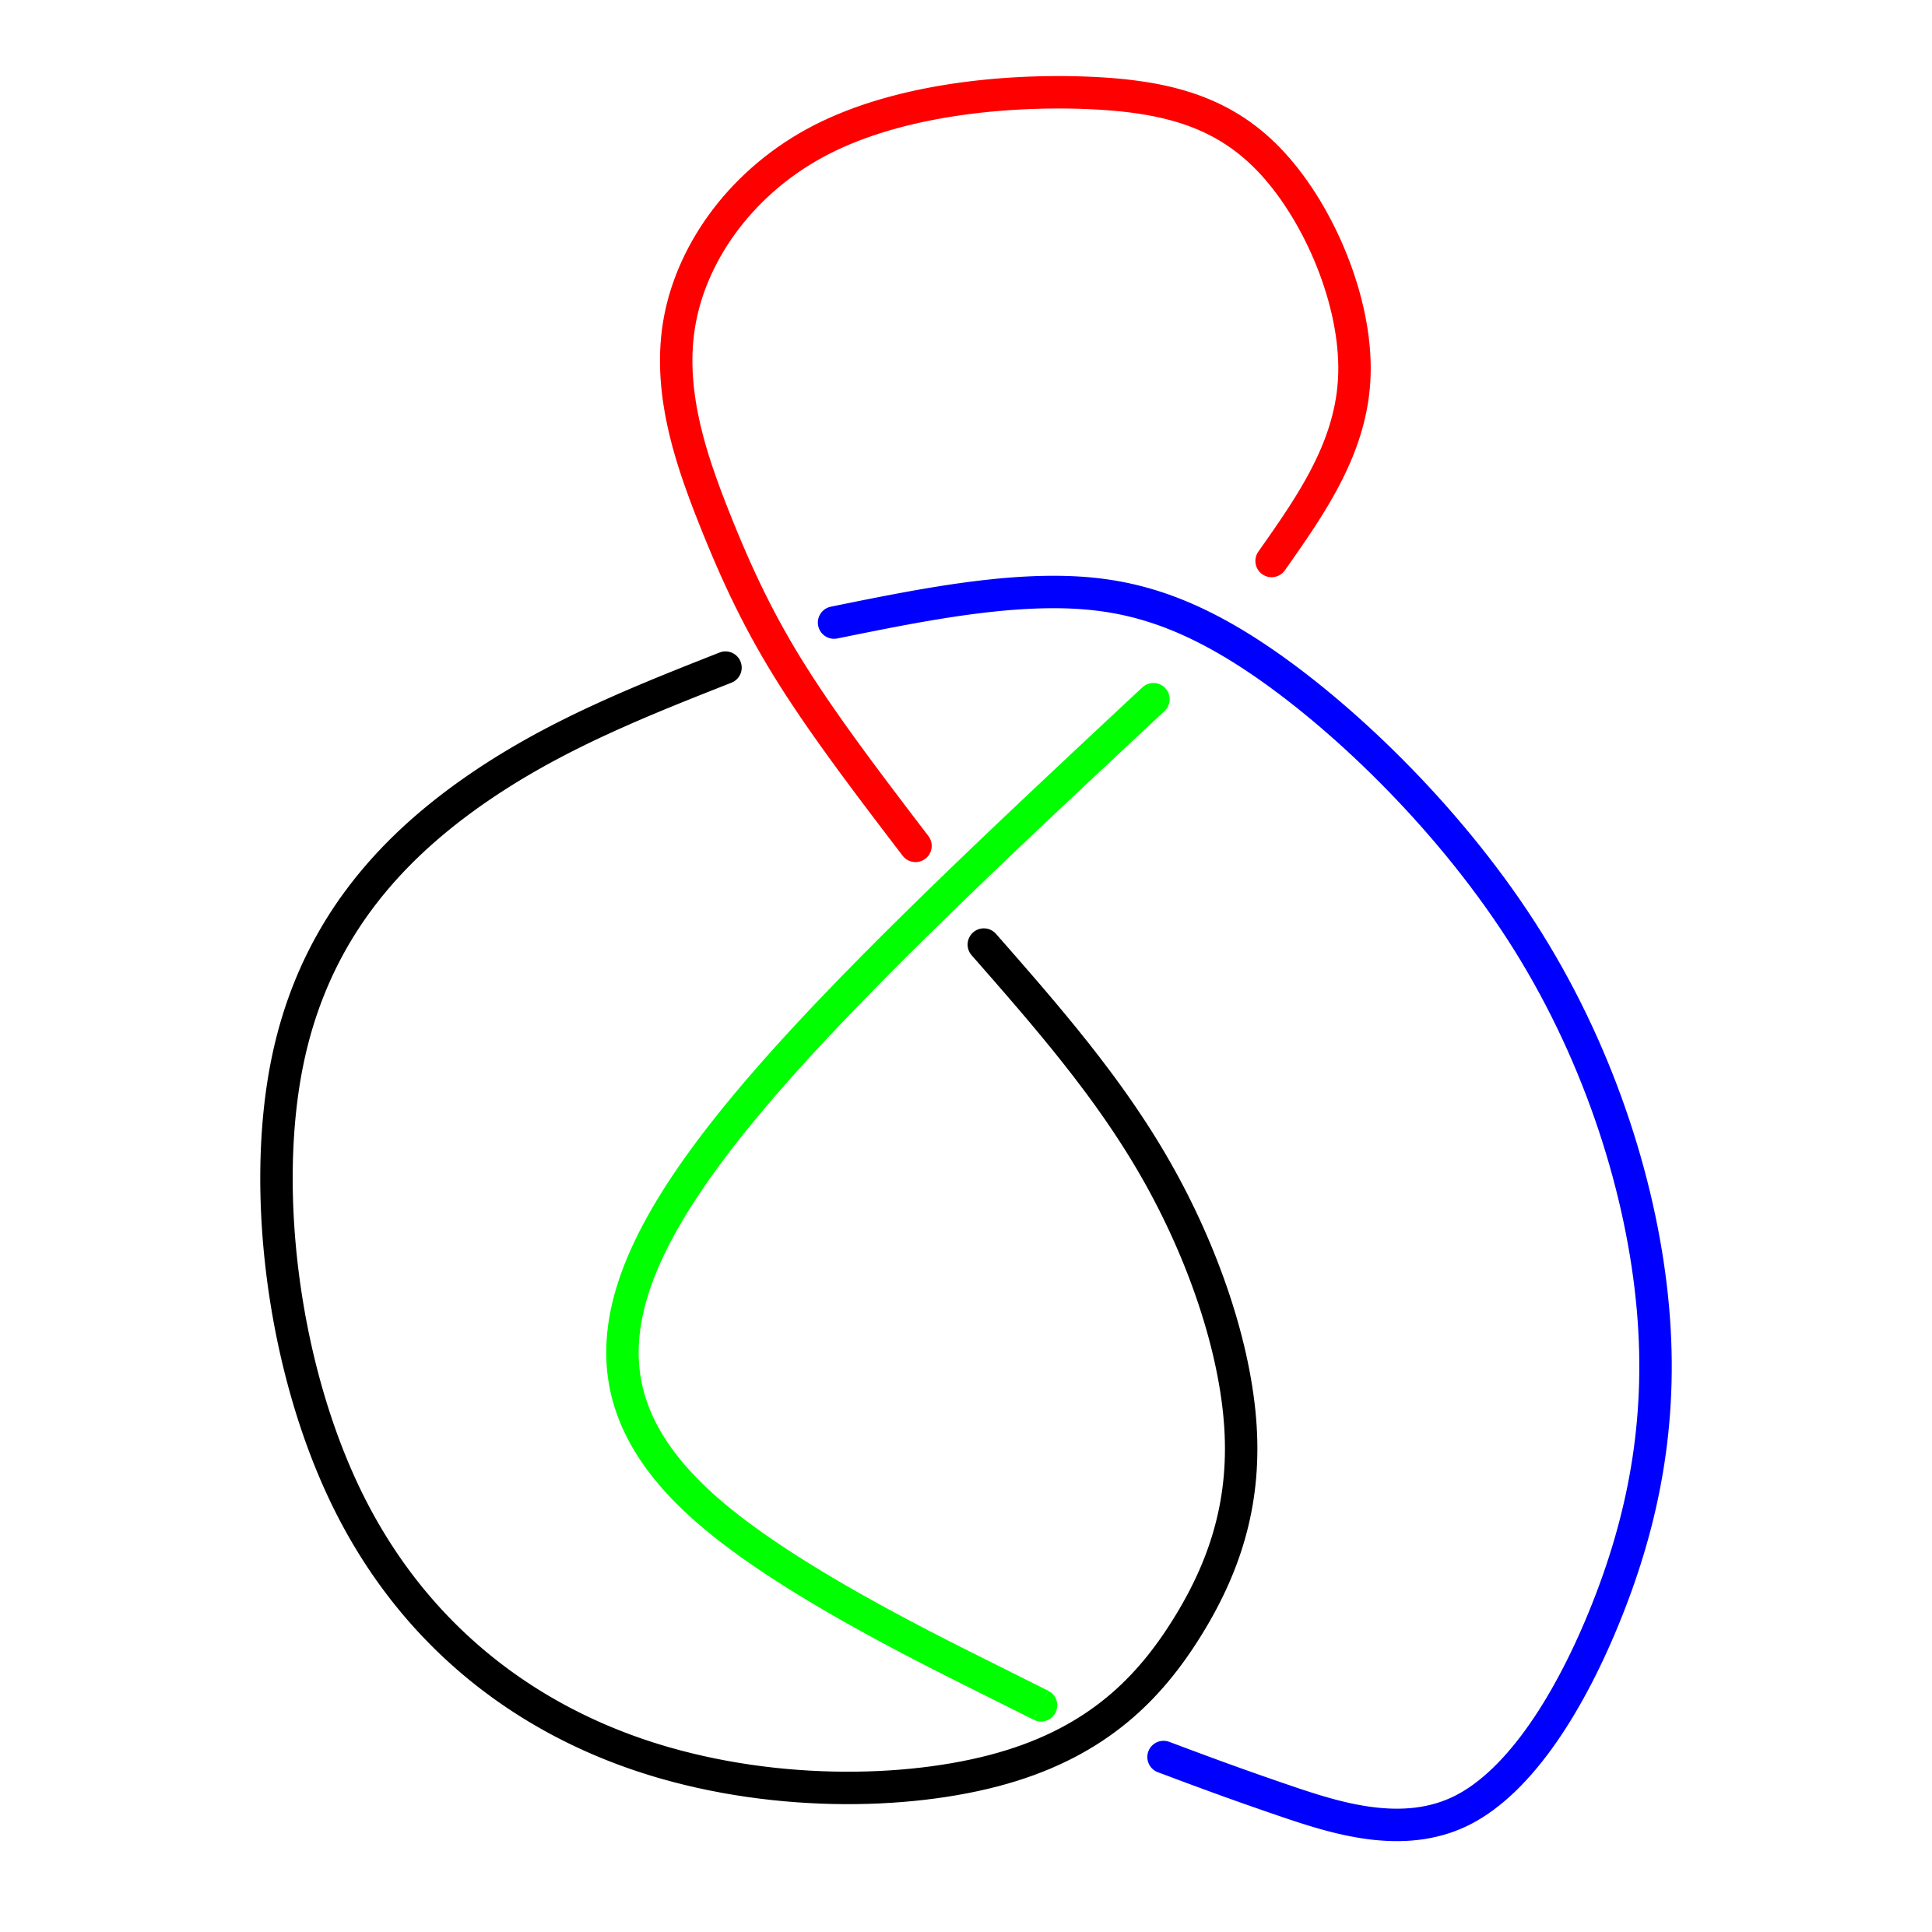
\includegraphics[width=0.5\linewidth]{picture/knotpict/knot-23}
	\caption{23rd Combination}
\end{subfigure}
\qquad
\begin{subfigure}[b]{0.25\linewidth}
	\centering
	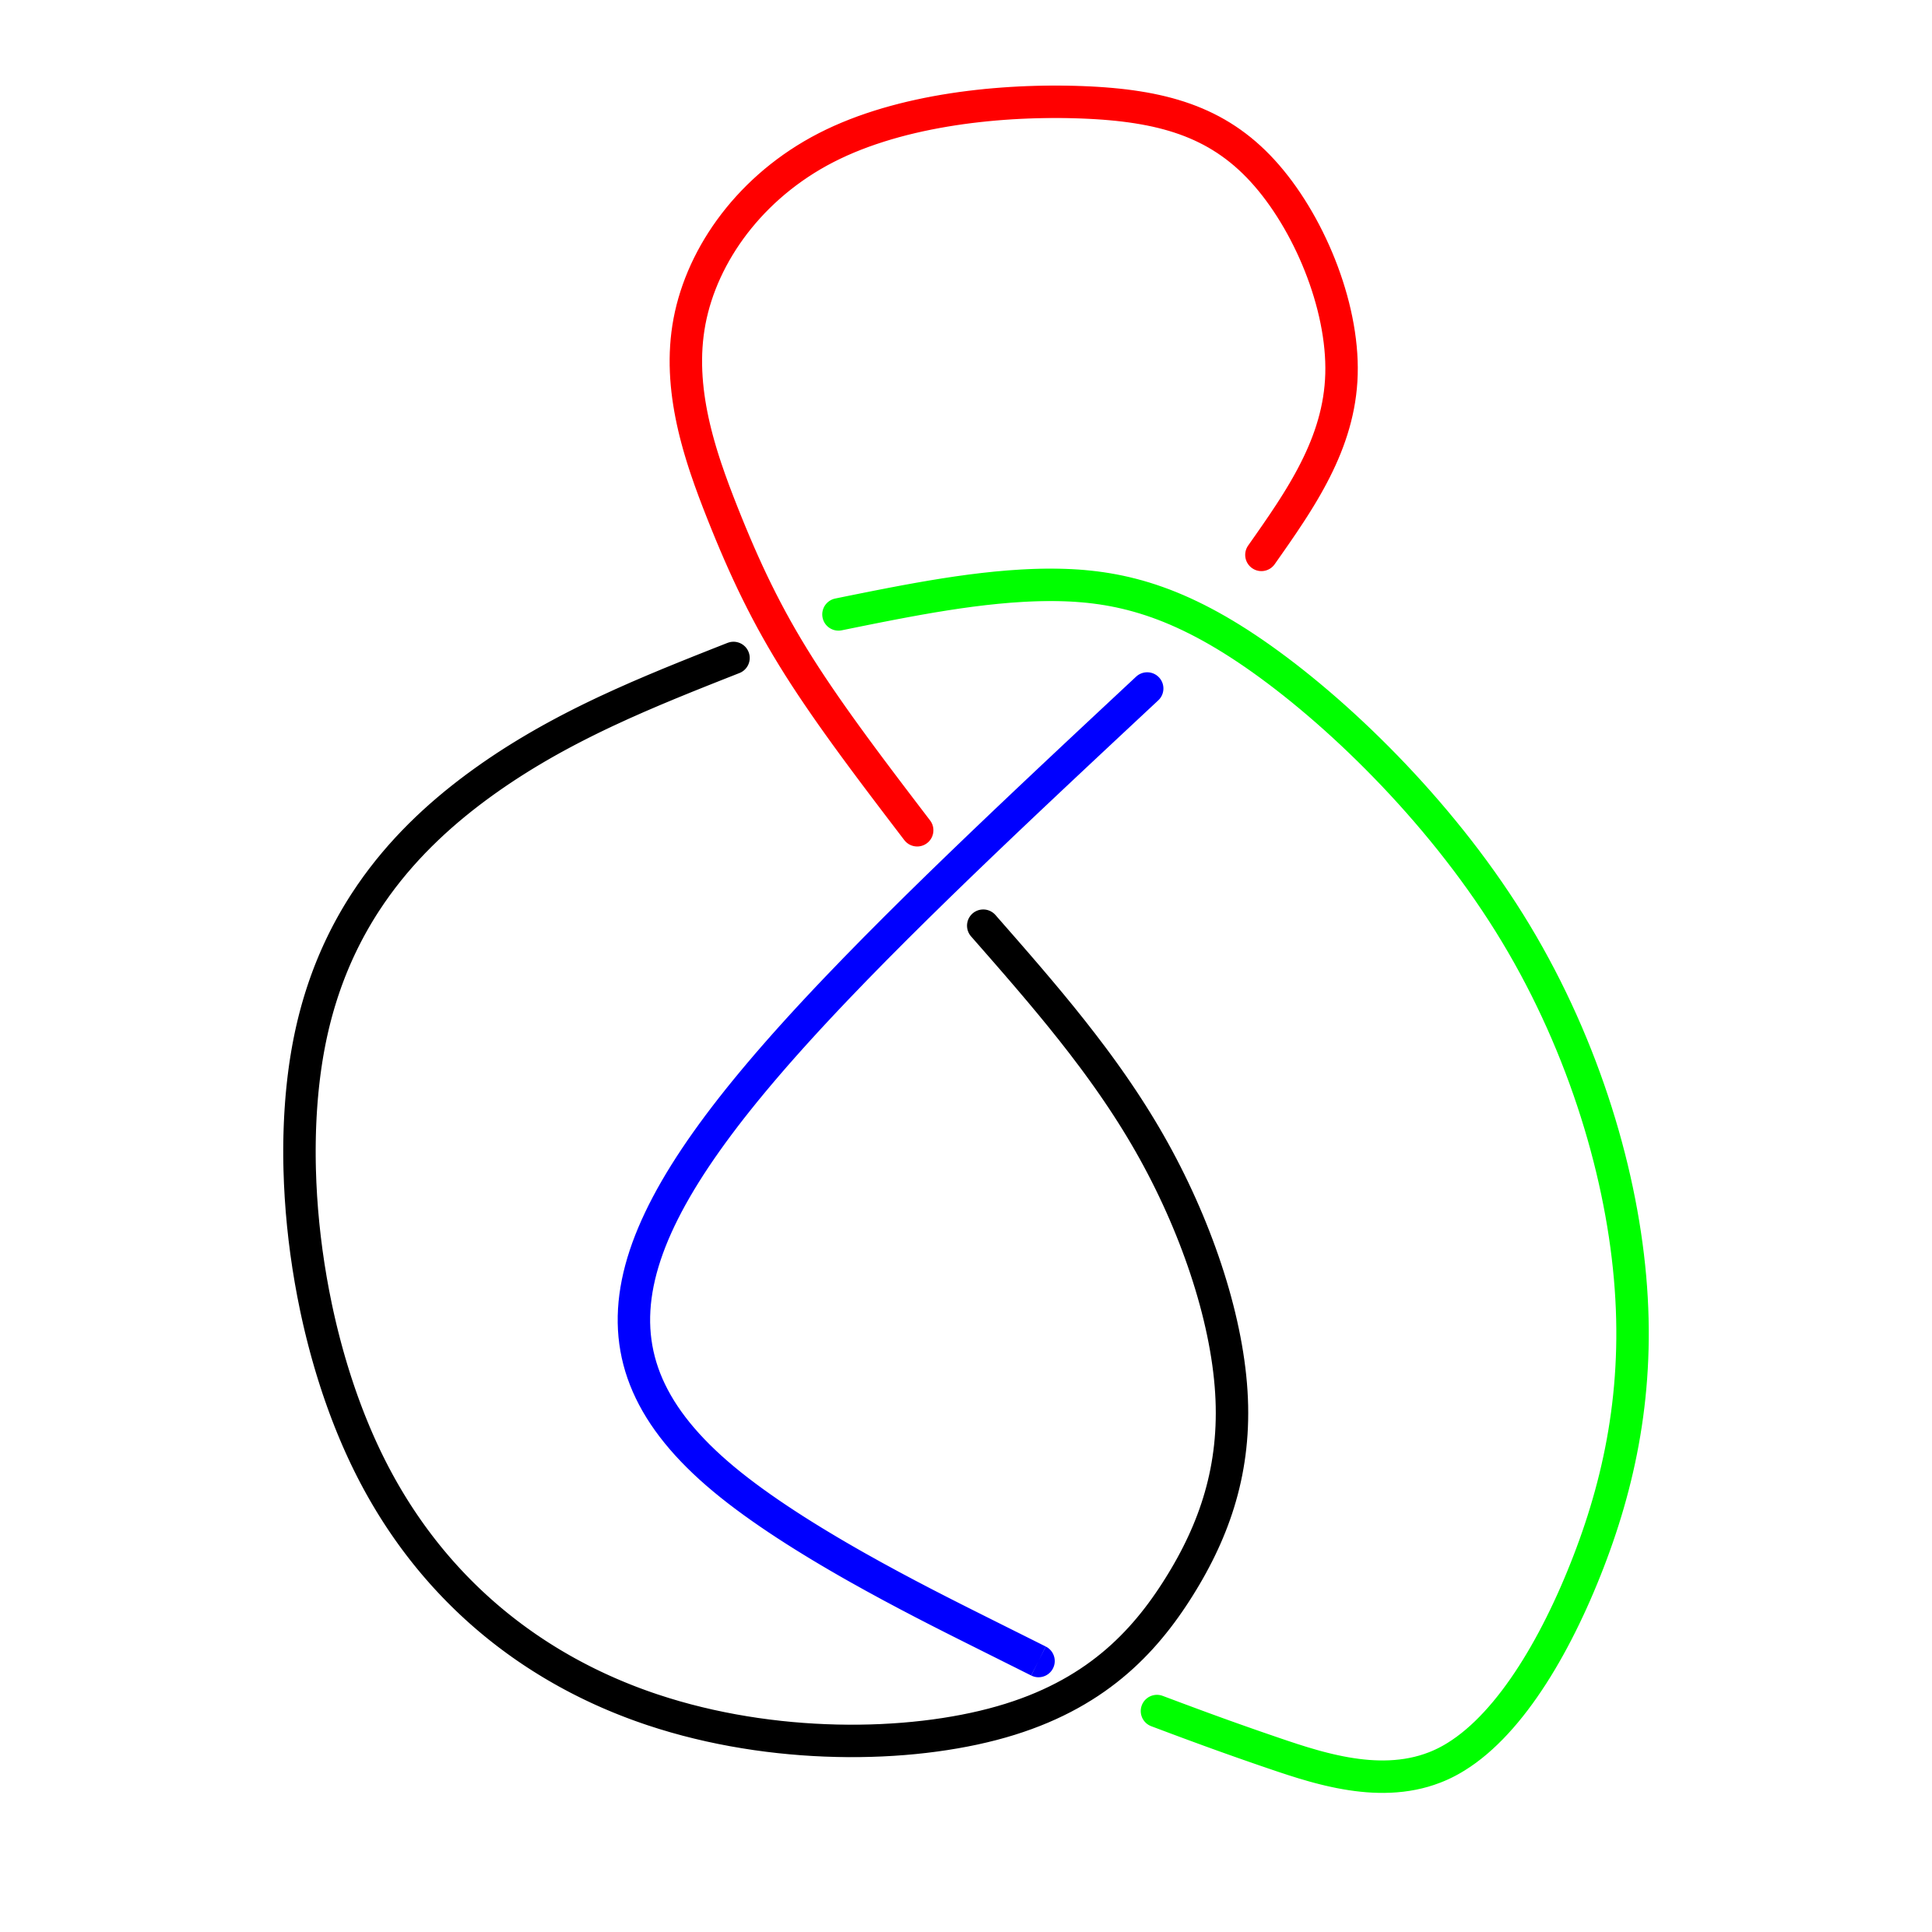
\includegraphics[width=0.5\linewidth]{picture/knotpict/knot-24}
	\caption{24th Combination}
\end{subfigure}
\caption{3 Colorings Combination of Figure-Eight Knot}
\label{fig:coloring knot}
\end{figure}
\newpage
Now for trivial colorings, we've shown in figure \ref{fig:trivialcolor} below:\\
\begin{figure}[h!]
	\begin{subfigure}[b]{0.3\linewidth}
		\centering
		
\includegraphics[width=\linewidth]{picture/knotpict/knot-25}
		\caption{25th Combination}
	\end{subfigure}
	\qquad
	\begin{subfigure}[b]{0.3\linewidth}
		\centering
		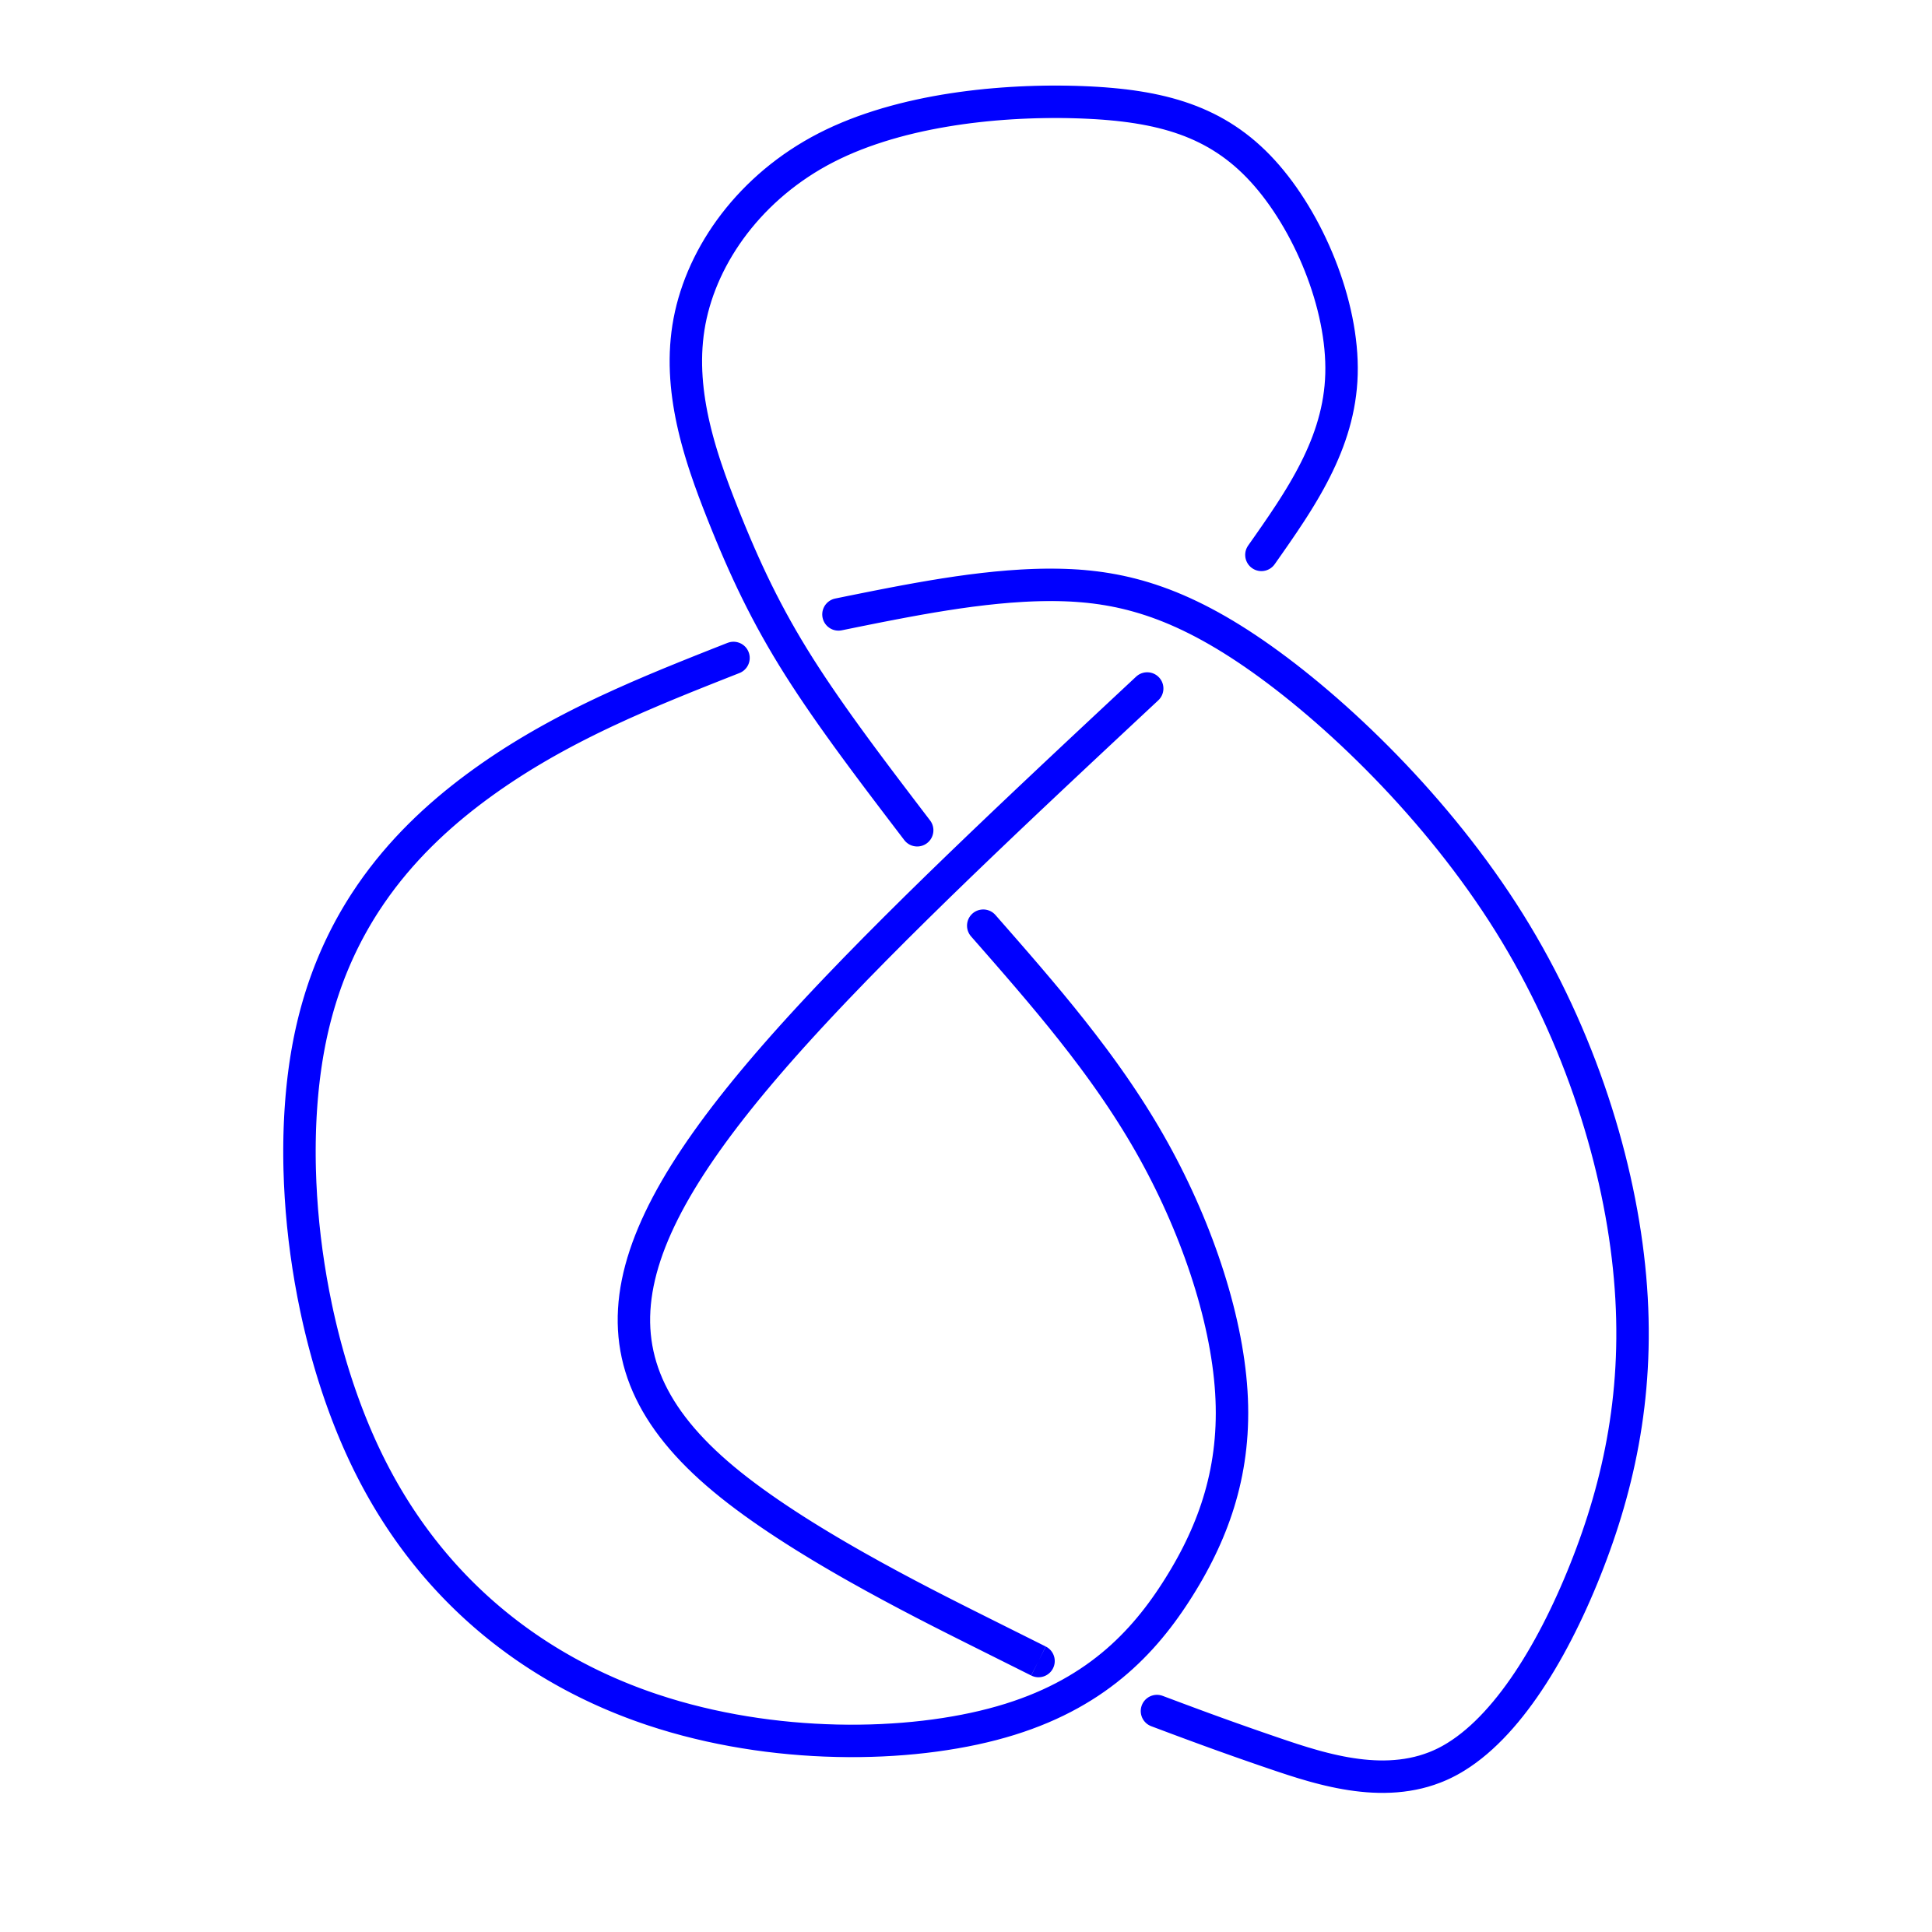
\includegraphics[width=\linewidth]{picture/knotpict/knot-26}
		\caption{26th Combination}
	\end{subfigure}
	\qquad
	\begin{subfigure}[b]{0.3\linewidth}
		\centering
		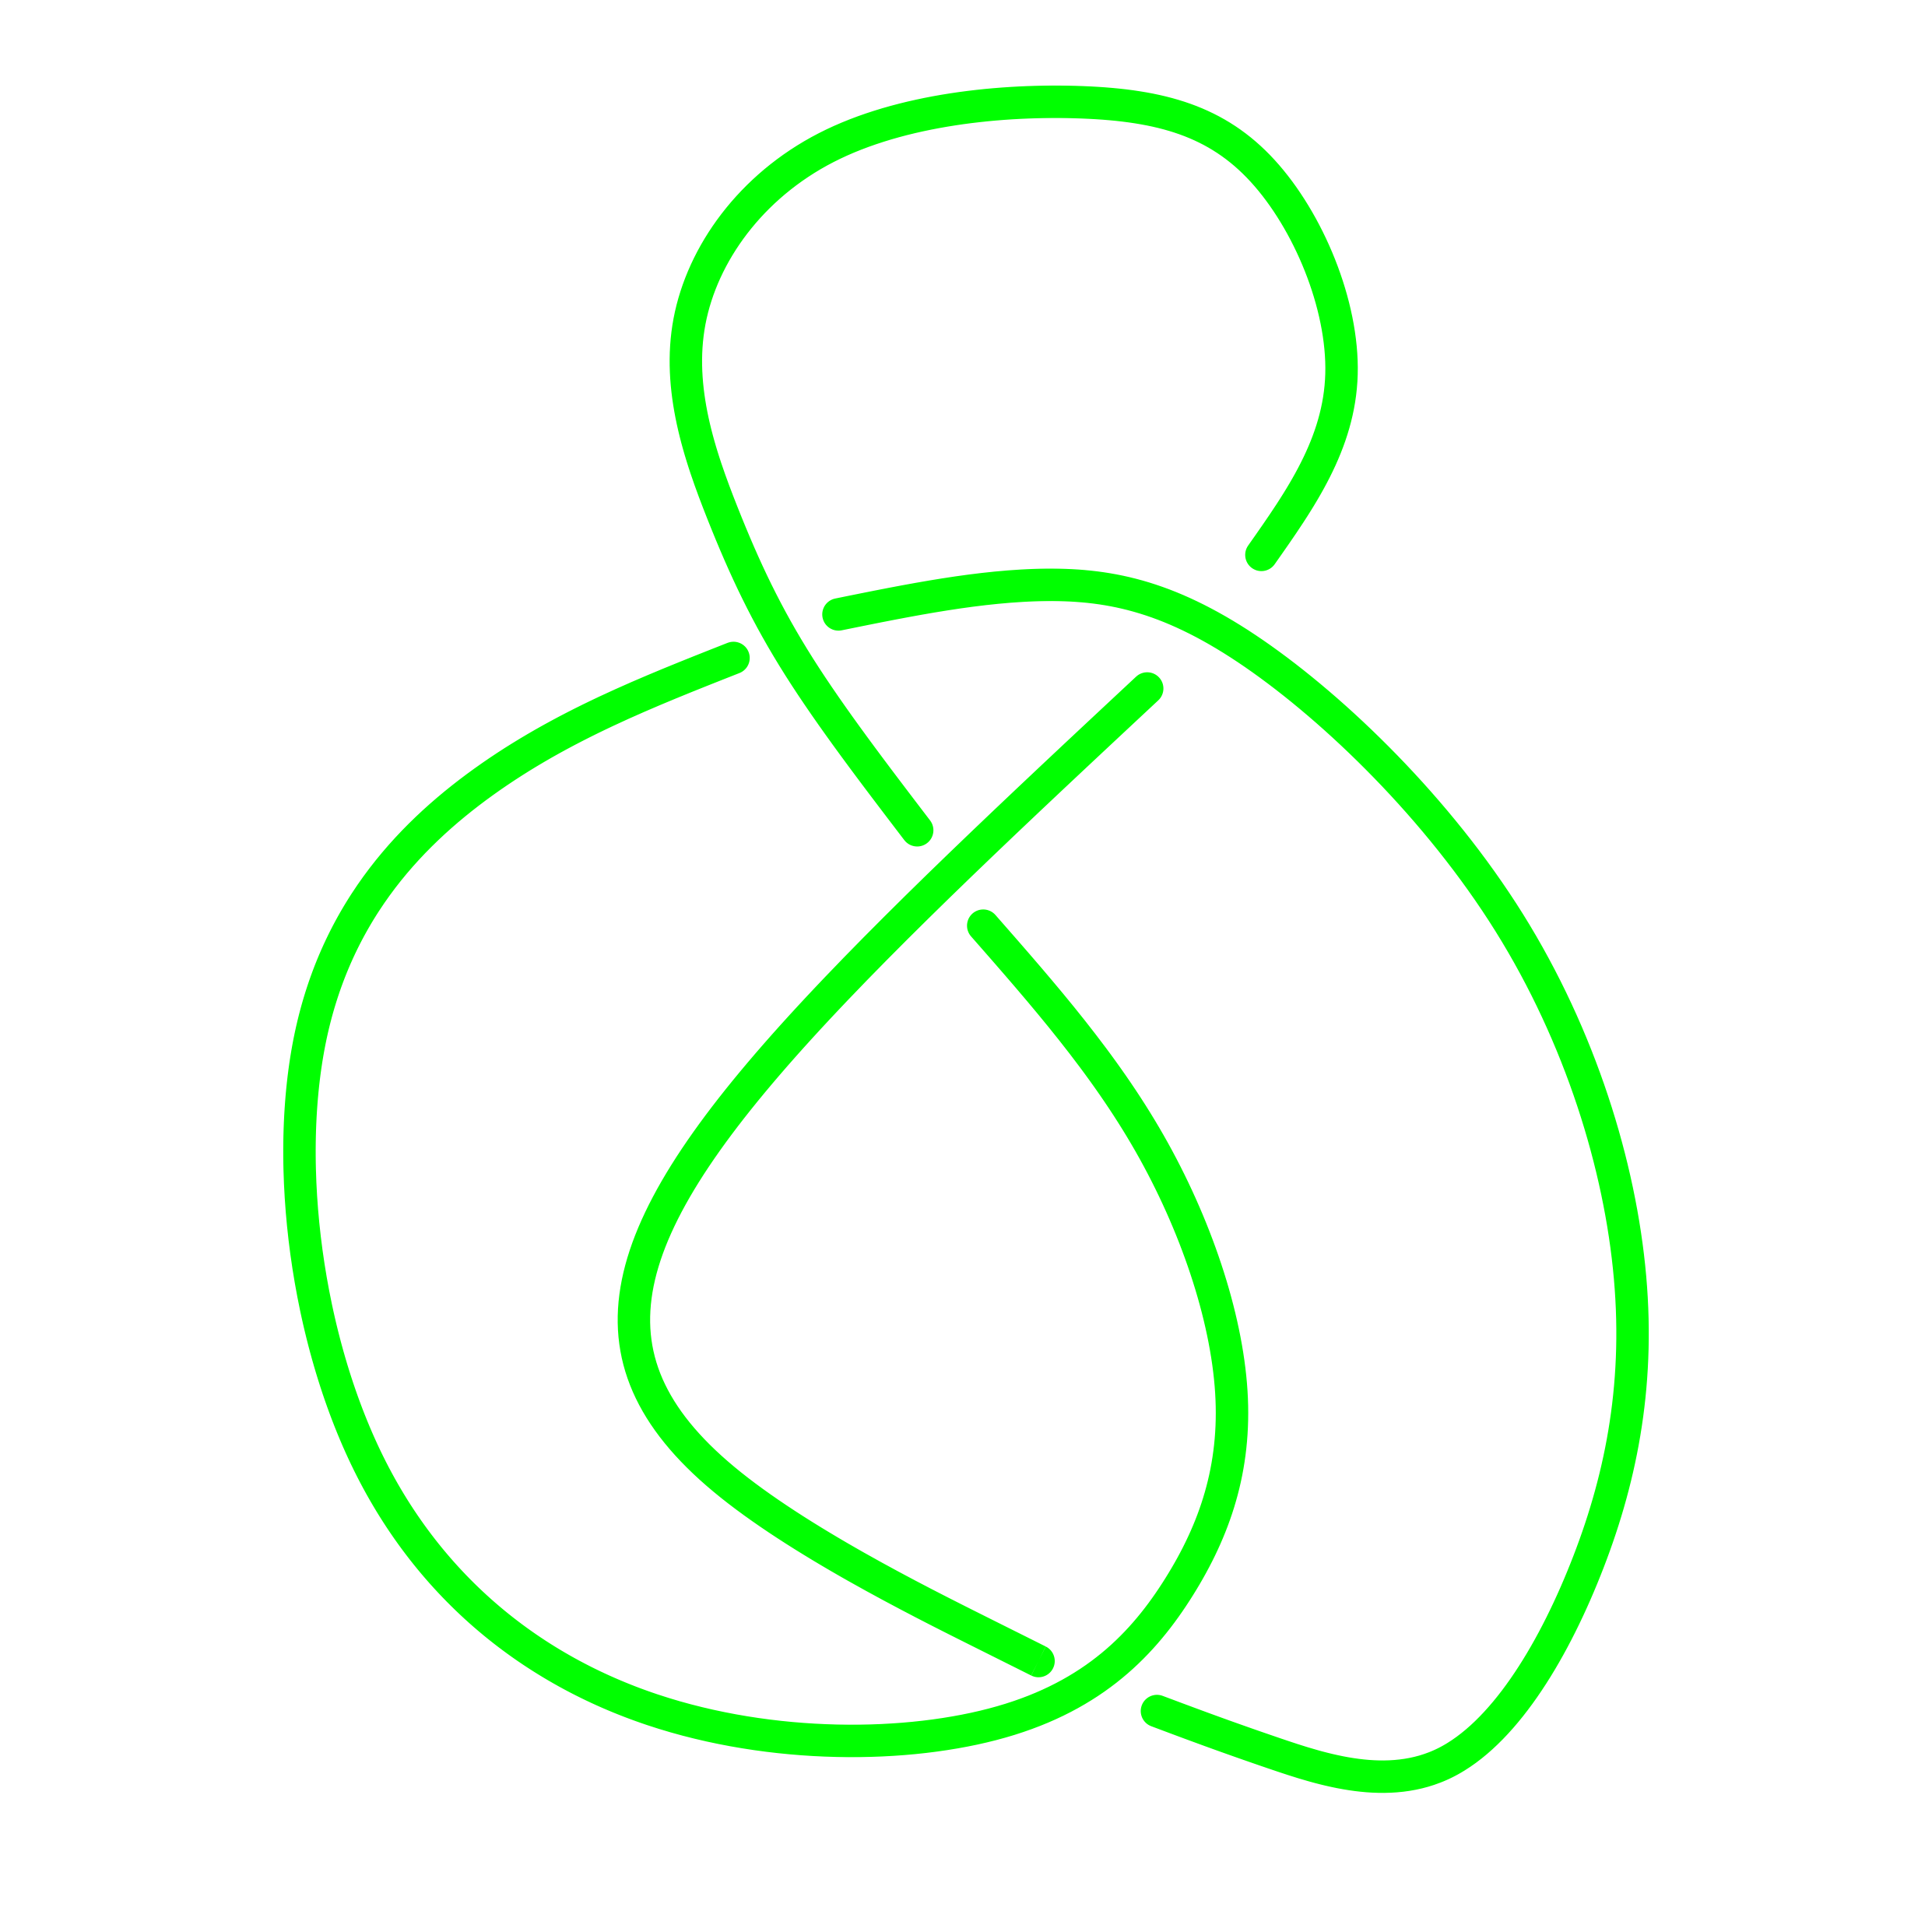
\includegraphics[width=\linewidth]{picture/knotpict/knot-27}
		\caption{27th Combination}
	\end{subfigure}
	\qquad
	\caption{Trivial Colorings Knot}
	\label{fig:trivialcolor}
\end{figure}
\newline
It is clear from figure \ref{fig:coloring knot} and \ref{fig:trivialcolor}, the colorings that satisfies definition of knot invariants, is just the \textbf{trivial colorings}, therefore there is \textbf{no 3-colorings} in \textbf{Figure-Eight Knot}, in other word, Figure-Eight Knot is not tricolorable because it has 4 edges with each pair of edge meeting at some crossing. If three of the edge had the same color, then all edge would be forced to be the same color. Otherwise each of these four edge must have a distinct color.
\end{enumerate}
\end{document}